%% ----------------------------------------------------------------
%% Thesis.tex -- MAIN FILE (the one that you compile with LaTeX)
%% ----------------------------------------------------------------

% Set up the document
\documentclass[a4paper, 11pt, oneside]{Thesis}  % Use the "Thesis" style, based on the ECS Thesis style by Steve Gunn
\graphicspath{Figures/}  % Location of the graphics files (set up for graphics to be in PDF format)


\usepackage[table,xcdraw]{xcolor}
\usepackage{fancyvrb}
% Include any extra LaTeX packages required
\usepackage[square, authoryear, comma]{natbib}  % 
%Use the "Natbib" style for the references in the Bibliography
%\usepackage[backend=biber,style=alphabetic,sorting=nyt]{biblatex}
\usepackage{verbatim}  % Needed for the "comment" environment to make LaTeX comments
\usepackage{vector}  % Allows "\bvec{}" and "\buvec{}" for "blackboard" style bold vectors in maths
\hypersetup{urlcolor=blue, colorlinks=true}  % Colours hyperlinks in blue, but this can be distracting if there are many links.

\newcommand{\bilinearroot}{Chapters/bilinear}

\newcommand{\fig}[1]{Figure~\ref{fig:#1}}
\newcommand{\pr}[1]{Problem~\ref{pr:#1}}
\newcommand{\sect}[1]{Section~\ref{sect:#1}}
\newcommand{\chapt}[1]{Chapter~\ref{chapt:#1}}
\newcommand{\tab}[1]{Table~\ref{tab:#1}}
\newcommand{\alg}[1]{Algorithm~\ref{alg:#1}}
\newcommand{\eq}[1]{(\ref{eq:#1})}
\newcommand*{\tran}{^{\mkern-1.5mu\mathsf{T}}}
\usepackage{verbatimbox}
\usepackage{todonotes}
\usepackage{gensymb}
\usepackage{enumitem}

%\usepackage{subfigure}
\usepackage{graphicx}
%\usepackage{caption}
% \usepackage{subcaption}
\newcommand{\ie}{\textit{i}.\textit{e}.,}
\newcommand{\eg}{\textit{e}.\textit{g}.,}
%\newcommand{\todo}[1][]{\@latex@warning{TODO #1}\fbox{TODO\dots}}


\usepackage{tabularx,lipsum,environ,amsmath,amssymb}
\newcounter{problemcounter}
\renewcommand{\theproblemcounter}{\arabic{problemcounter}}
\makeatletter
\newcommand{\problemtitle}[1]{\gdef\@problemtitle{#1}}% Store problem title
\newcommand{\probleminput}[1]{\gdef\@probleminput{#1}}% Store problem input
\newcommand{\problemquestion}[1]{\gdef\@problemquestion{#1}}% Store problem question
% \NewEnviron{problem}{
% \refstepcounter{problemcounter}
% \label{#1}%

%    \problemtitle{}
%    \probleminput{}\problemquestion{}% Default input is empty
%   \BODY% Parse input
%   \par\addvspace{.5\baselineskip}
%   \noindent
%   \begin{tabularx}{\textwidth}{@{\hspace{\parindent}} l X c}
%     \multicolumn{2}{@{\hspace{\parindent}}l}{Problem~\theproblemcounter. \textit{\@problemtitle}} \\% Title
%     \hline
%     \textbf{Input:} & \@probleminput \\% Input
%     \textbf{Task:} & \@problemquestion% Question
%     \\\hline
%   \end{tabularx}
%   \par\addvspace{.5\baselineskip}
% }

%\usepackage{amsmath,amssymb} % define this before the line numbering.
%\usepackage{placeins}
%\usepackage{color}
%\usepackage[width=122mm,left=12mm,paperwidth=146mm,height=193mm,top=12mm,paperheight=217mm]{geometry}
%\usepackage{subfigure}
%\usepackage{subcaption}
%\usepackage{xr-hyper}
%\usepackage[colorlinks=true]{hyperref}
%\usepackage{textcomp}

% Tikz-related stuff.
\usepackage{tikz}
\usetikzlibrary{arrows.meta}
\usetikzlibrary{backgrounds}
\usetikzlibrary{calc}
\usetikzlibrary{decorations.markings}
\usetikzlibrary{decorations.text}
\usetikzlibrary{fit}
\usetikzlibrary{positioning}
\usetikzlibrary{shapes.geometric}
\usetikzlibrary{3d}

% PGF-plots-related stuff.
\usepackage{pgfplots}
\usepgfplotslibrary{groupplots}
\pgfplotsset{compat=newest}

% \usepgfplotslibrary{external}
% \tikzexternalize

\usepackage{nomencl}
\makenomenclature
\renewcommand{\nomname}{List of Abbreviations}

\newcommand{\Sp}{{\mathcal S}^{+}}
\newcommand{\Sgen}{{\mathcal S}}
\newcommand{\Sm}{{\mathcal S}^{-}}
\newcommand{\spr}[2]{{\langle{}#1,#2\rangle}}
\newcommand{\prp}{p^{+}}
\newcommand{\prm}{p^{-}}
\newcommand{\Hp}{H^{+}}
\newcommand{\Hm}{H^{-}}
\newcommand{\hp}{h^{+}}
\newcommand{\hm}{h^{-}}

%%%%%%%%GRADREV HEADER


\usepackage{subfig}
\usepackage{algorithm}
\usepackage{algorithmic}
\usepackage{amsmath}
\usepackage{amssymb}
\usepackage{amsfonts}
\usepackage{dsfont}
\usepackage{xspace}
\usepackage{xr}
\usepackage{multirow}
\usepackage{multicol}
\usepackage{siunitx}
\usepackage{afterpage}
\usepackage{bbm}
\usepackage{enumerate}
\usepackage{booktabs}
\usepackage{natbib}
\usepackage{soul}
\usepackage{mathtools}
%\usepackage[colorlinks=false,allbordercolors={1 1 1}]{hyperref}
%\usepackage[hidelinks]{hyperref}

% Moscow header
%  \newcommand{\theHalgorithm}{\arabic{algorithm}}
\newcommand{\dataset}{{\cal D}}
\newcommand{\fracpartial}[2]{\frac{\partial #1}{\partial  #2}}

 
\def\x{{\mathbf x}}
\def\f{{\mathbf f}}

\def\S{{\cal S}}
\def\T{{\cal T}}

\def\R{{\mathds R}}

\def\tf{{\theta_f}}
\def\td{{\theta_d}}
\def\ty{{\theta_y}}
\def\htf{{\hat\theta_f}}
\def\htd{{\hat\theta_d}}
\def\hty{{\hat\theta_y}}
\newcommand{\ys}{y}
\newcommand{\yt}{y}

% uncertainty is separated with a "plus-minus" symbol
\sisetup{separate-uncertainty=true}

\usepackage{tikz}
\usetikzlibrary{positioning}
\usetikzlibrary{calc}

\usepackage{pgfplots}
\pgfplotsset{compat=newest} 
\pgfplotsset{plot coordinates/math parser=false}

% This is needed for plots.
\newlength\figureheight
\newlength\figurewidth


%\newcommand{\subfig}[1]{{\em(#1)}}

%\renewcommand{\topfraction}{0.85}
%\renewcommand{\textfraction}{0.1}
%\renewcommand{\floatpagefraction}{0.85}
%\parskip 0pt

\makeatletter
\makeatother


% Quebec's header


\newcommand{\phib}{{\pmb \phi}}
\newcommand{\uu}{{\mathbf{u}}}
%\renewcommand{\ww}{\uu}

\newcommand{\redplus}{``\red{$\boldsymbol{{+}}$}''}
\newcommand{\greenminus}{``\green{$\boldsymbol{{\pmb{-}}}$}''}

% To harmonize the transatlantic notation! 
% \renewcommand{\eqdef}{=}
\newcommand{\Acal}{{\mathcal{A}}}
\newcommand{\Xcal}{{\mathcal{X}}}
\newcommand{\Ycal}{{\mathcal{Y}}}
\newcommand{\Lcal}{{\mathcal{L}}}
\newcommand{\Dcal}{{\mathcal{D}}}
\newcommand{\Hcal}{{\mathcal{H}}}
\renewcommand{\Xcal}{X}
\renewcommand{\Ycal}{Y}
\newcommand{\dsum}{\displaystyle\sum}
\newcommand{\dprod}{\displaystyle\prod}


\DeclareMathOperator*{\argmax}{\mathrm{argmax}}
\DeclareMathOperator*{\argmin}{\mathrm{argmin}}

\newcommand{\DS}{{\Dcal_\textsc{S}}}
\newcommand{\DT}{{\Dcal_\textsc{T}}}
\newcommand{\DSX}{{\Dcal_\textsc{S}^{_\Xcal}}}
\newcommand{\DTX}{{\Dcal_\textsc{T}^{_\Xcal}}}

\newcommand{\RDS}{R_{\DS}}
\newcommand{\RDT}{R_{\DT}}
\newcommand{\RS}{R_{S}}
\newcommand{\RD}{R_{D}}
\renewcommand{\S}{\DSX}
\renewcommand{\T}{\DTX}
\newcommand{\xb}{{\mathbf x}}
\newcommand{\yb}{{\mathbf y}}



\usepackage{nomencl}
\makenomenclature
 
\renewcommand{\nomname}{List of abbreviations}

%%%%%%%%
\def\mystrut{\rule[-.3\baselineskip]{0pt}{0.5\baselineskip}}

\definecolor{inodefill}{HTML}{D9EAD3}
\definecolor{inodedraw}{HTML}{B6D7A8}
\definecolor{pnodefill}{HTML}{CFE2F3}
\definecolor{pnodedraw}{HTML}{9FC5E8}
\definecolor{onodefill}{HTML}{E6B8AF}
\definecolor{onodedraw}{HTML}{CC4125}
\definecolor{mnodefill}{HTML}{EAD1DC}
\definecolor{mnodedraw}{HTML}{D5A6BD}
\definecolor{goldfill}{HTML}{EAD7AC}
\definecolor{golddraw}{HTML}{D1AC71}
\definecolor{bluefill}{HTML}{5AB1F2}
\definecolor{bluedraw}{HTML}{0083E5}


%% ----------------------------------------------------------------
\begin{document}

\begin{titlepage}
 \begin{center}
 \phantom{a}\vspace{3.2cm}
 

\includegraphics[width=6cm]{sk.png}
  
  \large% SKOLKOVO INSTITUTE OF SCIENCE AND TECHNOLOGY
  \vspace{3.2cm}
  
  {\LARGE\bf Deep learning systems for 3D Reconstruction problems}
  \vspace{3cm}
  
  { \sl Doctoral Thesis\medskip
  
  by}\medskip
  
  Alexandr Notchenko
  \vspace{2cm}

  
  
  
 \end{center}

\end{titlepage}


\frontmatter      % Begin Roman style (i, ii, iii, iv...) page numbering

% Set up the Title Page
\title  {Deep learning systems for 3D Reconstruction problems}
\authors  {Alexandr Notchenko}
\addresses  {\groupname\\\deptname\\\univname}  % Do not change this here, instead these must be set in the "Thesis.cls" file, please look through it instead
\date       {\today}
\subject    {}
\keywords   {}

\maketitle
%% ----------------------------------------------------------------

\setstretch{1.3}  % It is better to have smaller font and larger line spacing than the other way round

% Define the page headers using the FancyHdr package and set up for one-sided printing
\fancyhead{}  % Clears all page headers and footers
\rhead{\thepage}  % Sets the right side header to show the page number
\lhead{}  % Clears the left side page header

\pagestyle{fancy}  % Finally, use the "fancy" page style to implement the FancyHdr headers

%% ----------------------------------------------------------------
% Declaration Page required for the Thesis, your institution may give you a different text to place here
%\Declaration{

%\addtocontents{toc}{\vspace{1em}}  % Add a gap in the Contents, for aesthetics

%I, AUTHOR NAME, declare that this thesis titled, `THESIS TITLE' and the work presented in it are my own. I confirm that:

%\begin{itemize}
%\item[\tiny{$\blacksquare$}] This work was done wholly or mainly while in candidature for a research degree at this University.

%\item[\tiny{$\blacksquare$}] Where any part of this thesis has previously been submitted for a degree or any other qualification at this University or any other institution, this has been clearly stated.

%\item[\tiny{$\blacksquare$}] Where I have consulted the published work of others, this is always clearly attributed.

%\item[\tiny{$\blacksquare$}] Where I have quoted from the work of others, the source is always given. With the exception of such quotations, this thesis is entirely my own work.

%\item[\tiny{$\blacksquare$}] I have acknowledged all main sources of help.

%\item[\tiny{$\blacksquare$}] Where the thesis is based on work done by myself jointly with others, I have made clear exactly what was done by others and what I have contributed myself.
%\\
%\end{itemize}


%Signed:\\
%\rule[1em]{25em}{0.5pt}  % This prints a line for the signature

%Date:\\
%\rule[1em]{25em}{0.5pt}  % This prints a line to write the date
%}
%\clearpage  % Declaration ended, now start a new page

%% ----------------------------------------------------------------
% The "Funny Quote Page"
%\pagestyle{empty}  % No headers or footers for the following pages

%\null\vfill
% Now comes the "Funny Quote", written in italics
%\textit{``You're just too good to be true \\
%Can't take my eyes off you.''}

%\begin{flushright}
%Bob Crewe, Bob Gaudio
%\end{flushright}

%\vfill\vfill\vfill\vfill\vfill\vfill\null
%\clearpage  % Funny Quote page ended, start a new page
%% ----------------------------------------------------------------

% The Abstract Page
\addtotoc{Abstract}  % Add the "Abstract" page entry to the Contents
\abstract{
\addtocontents{toc}{\vspace{1em}}  % Add a gap in the Contents, for aesthetics


This work considers 3D reconstruction problems, mainly a task of recreating a scene with many objects of different nature such as indoor structure of buildings, furniture, common objects and human bodies. Current state-of-the-art systems are highly specialised in processing a specific subset of objects uniform in their spatial and visual properties, and they don't generalize well outside of it's subset.

Computing relevant spatial features for sensor data is a crucial problem for Deep Learning based 3D reconstruction pipelines. Choice of scene representation for predictions and reconstructions also imensly importnant. Controling the domain to which different models compute predictions from sensor data, leads to a new level of quality, accuracy and applicability. This work pruposes a conceptual framework which unifyes 3D reconstruction models and provides ways to improve these models to solve their repsective tasks.


While deep learning has approached super-human performance in 2D image recognition, the results for 3D reconstruction have been relatively modest during recent years. Multiple improvements to 3D reconstruction methods are presented in this work. First one is an approach to learn effective embeddings used for retrieval of shapes in a large-scale database. Second one is a method for solving problem of fidelity for depth images using geometrically plausable prior. Third an imporvement to Dense Pose reconstruction from images algorithm, making it possible to run the model on embedded and mobile devices efficiently. Finally, a problem of 3D reconstruction from parts is adressed, by introducing a new dataset, and a methodology to infer objects from scans of real-world scenes using parts and inductive bias learned from a new dataset.


}

\clearpage  % Abstract ended, start a new page
%% ----------------------------------------------------------------

{\large
 List of publications:}


\begin{itemize}
    \item
    % A. Notchenko, E. Kapushev, \& E. Burnaev. Large-Scale Shape Retrieval with Sparse 3D Convolutional Neural Networks // AIST-2017, Lecture Notes in Computer Science, Springer
    Alexandr Notchenko, Yermek Kapushev, and Evgeny Burnaev. "Large-scale shape retrieval with sparse 3d convolutional neural networks." In International Conference on Analysis of Images, Social Networks and Texts, pp. 245-254. Springer, Cham, 2017.
    \textit{Personal contribution: developing the variant of the method for shape retrieval, designing and conducting the experiments for feature learning, text writing}

    \item
    % Voinov, O., Artemov, A., Egiazarian, V., Notchenko, A., Bobrovskikh, G., Zorin, D., \& Burnaev, E. Perceptual Deep Depth Super-Resolution. Proceedings of the IEEE international conference on computer vision. 2019.
    Oleg Voynov, Alexey Artemov, Vage Egiazarian, Alexander Notchenko, Gleb Bobrovskikh, Evgeny Burnaev, and Denis Zorin. "Perceptual deep depth super-resolution." In Proceedings of the IEEE International Conference on Computer Vision, pp. 5653-5663. 2019.
    \textit{Personal contribution: existing approaches analysis, conducting the experiments, text writing.}
    
    \item
    Rakhimov, R, Bogomolov, E, Notchenko, A, Mao, F, Artemov, A, Zorin, D, Burnaev, E. Making DensePose fast and light. Proceedings of the IEEE Winter Conference on Applications of Computer Vision 2021.
    \textit{Personal contribution: existing approaches analysis, method development, designing the experiments, text writing.}

    \item 
    Alexander Notchenko, Vladislav Ishimtzev, Alexey Bokhovkin, Alexey Artemov, Denis Zorin, and Evgeny Burnaev. Part Segmentation of the real-world 3D Scenes. (unpublished) 2021.
    \textit{Personal contribution: existing approaches analysis, method development, designing and conducting the experiments, text writing.}
\end{itemize}


\clearpage
\setstretch{1.3}  % Reset the line-spacing to 1.3 for body text (if it has changed)

% The Acknowledgements page, for thanking everyone
%\acknowledgements{
%\addtocontents{toc}{\vspace{1em}}  % Add a gap in the Contents, for aesthetics

%The acknowledgements and the people to thank go here, don't forget to include your project advisor\ldots

%}
%\clearpage  % End of the Acknowledgements
%% ----------------------------------------------------------------

\pagestyle{fancy}  %The page style headers have been "empty" all this time, now use the "fancy" headers as defined before to bring them back


%% ----------------------------------------------------------------
%\lhead{\emph{Contents}}  % Set the left side page header to "Contents"
\tableofcontents  % Write out the Table of Contents

%% ----------------------------------------------------------------
%\lhead{\emph{List of Figures}}  % Set the left side page header to "List if Figures"
%\listoffigures  % Write out the List of Figures

%% ----------------------------------------------------------------
%\lhead{\emph{List of Tables}}  % Set the left side page header to "List of Tables"
%\listoftables  % Write out the List of Tables

%% ----------------------------------------------------------------
\setstretch{1.5}  % Set the line spacing to 1.5, this makes the following tables easier to read

%\clearpage  % Start a new page
%\lhead{\emph{Abbreviations}}  % Set the left side page header to "Abbreviations"
%\listofsymbols{ll}  % Include a list of Abbreviations (a table of two columns)
%{
% \textbf{Acronym} & \textbf{W}hat (it) \textbf{S}tands \textbf{F}or \\
%\textbf{LAH} & \textbf{L}ist \textbf{A}bbreviations \textbf{H}ere \\
%
%}

%% ----------------------------------------------------------------
%\clearpage  % Start a new page
%\lhead{\emph{Physical Constants}}  % Set the left side page header to "Physical Constants"
%\listofconstants{lrcl}  % Include a list of Physical Constants (a four column table)
%{
% Constant Name & Symbol & = & Constant Value (with units) \\
%Speed of Light & $c$ & $=$ & $2.997\ 924\ 58\times10^{8}\ \mbox{ms}^{-\mbox{s}}$ (exact)\\

%}

%% ----------------------------------------------------------------
%\clearpage  %Start a new page
%\lhead{\emph{Symbols}}  % Set the left side page header to "Symbols"
%\listofnomenclature{lll}  % Include a list of Symbols (a three column table)
%{
% symbol & name & unit \\
%$a$ & distance & m \\
%$P$ & power & W (Js$^{-1}$) \\
%& & \\ % Gap to separate the Roman symbols from the Greek
%$\omega$ & angular frequency & rads$^{-1}$ \\
%}
%% ----------------------------------------------------------------
% End of the pre-able, contents and lists of things
% Begin the Dedication page

\setstretch{1.3}  % Return the line spacing back to 1.3

%\pagestyle{empty}  % Page style needs to be empty for this page
%\dedicatory{For/Dedicated to/To my\ldots}

\addtocontents{toc}{\vspace{2em}}  % Add a gap in the Contents, for aesthetics


%% ----------------------------------------------------------------
\mainmatter	  % Begin normal, numeric (1,2,3...) page numbering
\pagestyle{fancy}  % Return the page headers back to the "fancy" style

% Include the chapters of the thesis, as separate files
% Just uncomment the lines as you write the chapters




\nomenclature{CNN}{Convolutional Neural Network}
\nomenclature{t-SNE}{t-distributed Stochastic Neighbor Embedding}
\nomenclature{SGD}{Stochastic Gradient Descent}
\nomenclature{ReLU}{Rectified Linear Unit}
\nomenclature{DML}{Deep Metric Learning}
 
 
\printnomenclature


% !TEX root = ../Thesis_main.tex
\chapter{Introduction}

%video surveillance+
%person re-id+
% originates from Multi-Target Multi-Camera Tracking 
%open world / closed world+
%face : verification/identification
%common aspects: detection , processing, recognition
%deep learning

%retrieval
%fine-grained recognition
%adaptation

%datasets (cut from the papers) + table with reid dataset?
%architectures
%definitions?
%contribution - what is done
\section{Context}
\subsection{Problem of 3D reconstruction}

\subsection{Approaches for solving 3D Reconstruction problem}

Solutions for a reconstruction problem can be grouped in two major groups: 1) Geometric approach - when problem is represented as optimisation of scene state given constrains on projections of scene state to data, 2) Machine Learning approach - inverse model is optimisation.

If $X$ - is scene data, $z$ - is the state of the scene, and $g_i(z)$ - projection function of 3D scene $z$ state to perspective $i$, then to find an optimal 3D reconstruction, one solves this minimisation problem:
\begin{equation}
z_{rec} = \min_z\sum_i|X_i-g_i(z)|_2 .
\end{equation}

This approach only solves problem for once scene and does not provide any semantic information about it, only basic geometric information. 
The second approach is more modern and better fitted for machine learning applications, because instead of optimizing state of the scene, it's optimizes a model that performs computation from input data to some semantic (intrinsic) parameters, and can be described as following optimisation procedure:
\begin{equation}
\min_\theta\sum_i|X_i-g_i(f_\theta(\pi))|_2,\ \ \pi=I_\theta(\{X_i\}_i),\ \ z=f_\theta(\pi),
\end{equation}
where $\pi$ - are scene parameters, $f_\theta(\pi)$ - is a generative model that generates 3D state $z$ and it's function is determined by tunable parameters $\theta$.

In reconstruction process information can be introduced in two possible ways: 1) input signal - data measured by some spatial sensor, 2) by adding a priori knowledge while training the Inverse model or by design choice of reconstruction algprithm. Between the two source exist a fundamental trade-off and detirmination of which is dominant can be quite difficult \cite{tatarchenko2019single}.


\subsection{Objectives and Motivations}

The goal of this work to improve methods of 3D reconstruction in holistic context using deep learning systems. For efficient applications such as robotics in human environments and mixed reality more advanced machine perception systems are needed. Human perception is a complex system with several properties not all of which are replicated in modern machine perception systems. From cognitive sciences it's known that ability to model environments is one of the most important for perception system, in area of computer vision this is known as an ability to perform \textit{3D reconstruction} of scenes and environments. To solve this problem in a general case requires application of machine learning.

In particular, the development of such holistic deep 3D reconstruction system includes several important tasks:

\begin{itemize}
􏰀    \item Capturing scenes, complete with colour and depth data of a sufficient quality,
    \item Recalling objects from large scale database of objects,
    \item Segmenting variety of most common elements from sensor data, such as household objects and architectural components,
    \item Detecting and reconstructing shape and pose of and human bodies.
\end{itemize}

Each of these sub-tasks constitutes a challenge in the context of human perception.

The presence of noise in sensor data (e.g., consumer grade depth cameras) is a serious problem for all downstream sub-tasks, low fidelity of this data causes a considerable compaunding performance drop.

\subsection{3D data representations}

We can describe a 3D object in multiple ways, and codification of it's properties has ramifications about capturing different information about objects and scenes, as well as kinds of models that can regenerate them or computational resources needed to process it.
Each representation has it's own pros and cons. We assume 3D information representation to be positive effective and usefull if it captures more relevant information with less storage requirement (compression), increases signal to noise ratio of data, captures shape and texture properties with minimum trade-off.

Here are some popular examples of 3D data representations:
\begin{enumerate}
	\item Multiple 2D projections - captures surface texture, highly redundant representation if images overlap, also vulnerable to optic illusions.
	\item Voxels - simple, most of the time can be sparse, represents rough volumetric properties vell but losses most of surface properties.
	\item Point Cloud - are sparse in a sense that they don't capture empty space, losing all surface properties besides color and estimated normals and most of volumetric properties.
	\item 2.5D (RGB-D) images are widespread because of cheap measurement devices, capture volumentric depth but succeptable to occlusion of bodies in a scene and records a lot of noise with actual signal.
\end{enumerate}



%Motivation: RGB-D scanning is here and we want to have a fine-grained understanding of the 3D captures
In the recent years, a wide variety of consumer-grade RGB-D sensors, such as the Intel Real Sense, Microsoft Kinect, depth-sensor enabled smartphones, enabled inexpensive and rapid RGB-D data acquisition. Increasing availability of large, labeled datasets (e.g.,~\cite{chang2017matterport3d,dai2017scannet})  made possible development of deep learning methods for 3D object classification and semantic segmentation. At the same time, acquired 3D data is often incomplete and noisy; while one can identify and segment the objects in the scene, reconstructing high-quality geometry of objects remains a challenging problem.  

An example of the new approach in recent work 
\cite{avetisyan2019scan2cad}, uses a large dataset of clean, labeled geometric shapes
\cite{chang2015shapenet}, for classification/segmentation associating the input point or voxel data with object labels from the dataset, along with adapting geometry to 3D data.  This approach ensures that the output geometry has high quality, and is robust with respect to noise and missing data in the input.  
At the same time, a ``flat'' classification/segmentation approach, with each object in the database corresponding to a separate label and matched to a subpart of the input data corresponding to the whole object, does not scale well as the number of classes grows and often runs into difficulties in the cases of extreme occlusion (only a relatively small part of an object is visible). 
Significant improvements can be achieved by considering object \emph{parts}, or more generally part hierarchies. 
Part-based segmentation of 3D datasets promises to offer a significant improvement both in finding the best matching shape in the dataset, recognizing objects from  highly incomplete data (e.g., from a couple of parts) from  as well as more precise geometry adaptation as well as, potentially, assembly of new shapes out of existing parts yielding a closer match to the input data. 

large collection of 3D models in database can be reduced to structured representations, 
objects with occluded sub-parts still can be recognized by parts available in the scan and the rest can be guessed with high probability, using parts, we can reconstruct new objects that are not yet present in the database of shapes.

Based on different approaches for volumetric information integration, from enhancements of  methods such as volumetric fusion \cite{curless1996volumetric}, to probabilistic  methods, and plethora of methods based on their combinations.

Compared to computer graphics models manually created by 3D professionals, 3D scans are noisy and incomplete.
Amount of noise and limited resolution of consumer-grade scanning hardware pose significant challenges for solving this important problem of scene reconstruction. 
Approaches of reconstruction based on fitting existing 3D assets into scene scans, have shown a lot of promise but still had problems with finding exact models from large database such as ShapeNet \cite{chang2015shapenet}, because of occlusion and lack of spatial context.

Learning-based approaches are very good at extracting features representative of objects and scenes as a whole, allowing to fill in occluded areas or guess parts affected by noise \cite{dai2017shape,dai2018scancomplete,song2017semantic}. These features are sufficient for scene completion, but they are not as good at recovering geometric primitives like: sharp edges, planar surfaces or borders between sub-parts, resulting in reconstruction quality much poorer than that of 3D content created by humans.

In this work, we focus on the key problem of semantic part segmentation of objects in the scenes, enabling further improvements in  dataset-based reconstruction. 
Semantic part-segmentation, can help in these situations, when sufficient number of the object parts is visible model can infer the non-visible parts essentially completing an object in sense of maximum probability conditioned on input data.

In human-made environments, a lot of objects have naturally defined semantic sub-parts, and those sub-parts can, in turn, have their sub-parts, i.e., parts form \emph{hierarchies}.  In our work, we use scene and object representation based on such part hierarchies.  We show how a part-labeled dataset of scanned 3D data suitable for machine learning applications can be constructed, and used to improve the performance of segmentation algorithms. 

Definitions of sub-parts are based on a set of primitive elements that were manufactured by one formation method or from one material.

Because of that and the fact that static scenes have other relationships between objects (fixed to each other or in direct surface contact), it's reasonable to suggest a scene description format that possesses a property of hierarchy (e.g., trees or other kinds of graphs).
Representing scenes as a discrete structures with multiple relationships between nodes. Such relationships like composability of its parts and affordances between whole objects, in turn allowing to compose a scene from separate objects.

\todo{merge these paragraphs}

In domain of human-made environments a lot of objects have sub-parts and those sub-parts can in turn have their own sub-parts. Definition of sub-part is often based on a set of primitive elements that were manufactured by one formation method or from one material. Because of that and the fact that static scenes have other relationships between objects (fixed to each other or in direct surface contact), it's reasonable to suggest a scene description format that possess a property of hierarchy (e.g. trees or other subgraphs).
A lot of researchers over the last 20 years came to the same conclusion. A lot of work on that problem was done by Mumford and Zhu in \cite{zhu2006stochastic}.

One of the papers dealt with problem of modeling Images as a hierarchy of super-pixels. \cite{russell2009associative}, or as a tree of geometric primitives (e.g. cylinders, spheres or 3D boxes) \cite{li2017grass}.

% point cloud (PC) turned in to a graph (based on proximity) point-cloud parser network reduces number of nodes and edges and enriches their feature vectors. First part of the decoder network functions similar to Feature Pyramid Network in CNNs, which performs local computations on different scales, followed by "pooling or convolutions" with reduced spatial component and increased feature components, thus leaving only small number of "keypoints" required to outline shapes of objects.



CAD constructor network translates that graph into CAD object (tree with primitives and combination rules). CAD rendered makes a mesh out of that object thus a residual between original PC and Mesh can be calculated.

Proximity Graphs - concept that allows to build a bridge between Point Clouds and Graph Processing. This area of computational geometry has a lot of theoretical results to offer for Deep Learning piplene designer.


\subsection{Definitions and examples}
\subsection{Data sources and devices}

\section{Inverse Graphics Problem formulation}

\cite{rezende2016unsupervised,eslami2016attend,kulkarni2015deep,wu20153d,izadinia2017im2cad}

Inverse graphics approach enables to solve a problem of "real-world" scene understanding through reconstruction of that scene and comparison it to measured data in some form.

Because it's a fairly new method it has some unexplored facets:
\begin{enumerate}
    \item How can we scale to hundreds and thousands of objects with different parameters.
    \item Embedded representations better than procedural generation
    \item Are there format that can have all advantages of CAD models and probabilistic properties that arise from real-world uncertainties.
\end{enumerate}

Central goals of computational perception is to get structured description of scenes from measurements such as photographic images, scans and videos.

Computer Vision as Inverse Graphics is the most rational formulations that could help us achieve this goal.

In the past, it has been hard to directly solve these problems in practice because of computational limitations.

However, it may be right time to take another look at this idea due to significant advances in deep learning for computer vision, probabilistic programming, and computer graphics.

Probabilistic programming - a tool that allows us to implement complex models while keeping ability to perform inference, extend with other probabilistic models by being general-purpose.

Re-formalizing inverse graphics in terms of probabilistic programming and deep learning allow us to solve even more complicated vision problems with off-the-shelf computational technology.

To make this approach scalable, my research can incorporate effective techniques such as: approximate Bayesian computation, differentiable programming for rendering.

Computer Graphics nowadays seems to be improving at a great pace in terms of designing solutions for hard image synthesis problems, but these solutions are usually hand-made and not flexible enough to cover all needs for general-purpose real world object generating, latest advances in generative models can help with that.


\subsection{Overcoming lack of information}

\section{Datasets}

Only recently research community started accumuulating sugnifficant amount of algined sensor data to solve large scale 3D reconstruction problems in deep learning context. In last 4 years we saw an explosion of 3D shape databases and 2D-to-3D indoor scene datasets, such as ShapeNet, 2D-3D Semantic, Scannet and Matterport3D datasets. Because accuracy and reacall properties of deep learning models scale with amount and variety of data, number of state-of-the-art models grew as well.

\section{Architectures}

PanopticFusion~\cite{narita2019panopticfusion} is a model that is able to segment large indoor scenes and separate \textit{Stuff} and \textit{Things}.


For outdoor datasets Point Cloud representation of data is more common because of large empty spaces and the way LiDAR sensor collects data. In such setting instance segmentation is nessesary first step for reconstruction~\cite{zhang2020instance}.

\subsection{Multi-view models}

Detailed comparision of multi-view 2D CNN model and 3D volumetric CNN can be found in \cite{qi2016volumetric}.

\subsection{Implicit 2D models}

Like inverse graphics network. Model takes 2D images and returns 2D images with 3D properties changed. 

\subsection{3D convolutional models}

Model generates or processes voxel image with 3D convolutional operation implemented Dense or Sparse.

Semantic information can boost the reconstruction performance because deep learning systems are able to pick up onto consistent signal \cite{jiao2018look,tatarchenko2019single,kendall2018multi}.

\subsection{2D to 3D Projection models}

Model uses camera parameters to compute 3D representation using 2D/2.5D images and projection operation.

\subsection{Point Set layers}

Neural Network processes a set of points to classify, segment or predict new set of points.

\subsection{Graph-Convolutional layers}

Model processes Geometric Graph where nodes represent points registered on a surface of objects or parts of objects, and has geometric or other information representing edges between points. Layers process activations associated with nodes taking into account the connectivity.

\subsection{Differentiable rendering layers}

Rendering operation is implemented in a differentiable way, allowing backpropogation of gradient information from 2D images to meshes and textures of the objects being rendered.

\subsection{Mesh generating layers}

Neaural Network layers that can create a mesh by way of processing a template 3D shape with parametracised operation or meshing other 3D shape representation generated by computation from weights and input.

\subsection{Implicit 3D models}

Models like NeRF, PIFU3D, neural network implements a rendering function depending on view angle and other graphics parameters, one model represents one scene and don't generalise for viriety of scene inputs.



\section{Contributions}

% \chapt{hist}, \chapt{bilinear} and \chapt{gradrev} use  person re-identification architecture of \citep{Yi14} as a baseline method (it is also  described in \sect{intro_architectures}).  \chapt{bilinear} is based on the results of \chapt{hist}: the loss function introduced in \chapt{hist} is used for 
% all the experiments in \chapt{bilinear} as it was demonstrated to show the best performance for person re-identification. 
% The results of \chapt{gradrev} were chronologically the earliest among all the results presented in this work, therefore  methods  from \chapt{hist} and \chapt{bilinear} were not used there. 
% Although the contributions of each of the chapters are independent, they are all parts of building a person re-identification pipeline and can be applied simultaneously. 
% \chapt{wildface} considers domain adaptation for surveillance face recognition and uses the method from \chapt{gradrev} as one of the baselines.
 


\newpage 
\chapter{Related work}

\section{Shape Retrieval}
\label{sec:shape_retrieval}

Many papers about how to take a codified shape of an object or scanned data and find record in a shape database. Many aspects related to completeness of database and other retrieval problems.


\section{Geometric Reconstruction}
\label{sec:geometric_reconstruction}

About SLAM methods or bundle adjustment problems where the semantic properties or nature of objects is not known.

\section{Human Body Shape Reconstruction}
\label{sec:body_reconstruction}

About body shape regression and dense pose estimation.

\section{Retrieval-based Reconstruction}
\label{sec:retrieval_reconstruction}

Scan2Cad and simmilar methods which use retrival as way to "explain" registered signals.

\section{Uncertainty in Reconstruction}
\label{sec:uncertainty_reconstruction}

About role of prior knowledge and how it's represented in various models. a tie-in with deep depth-image prior.

\section{Part-aware Reconstruction}
\label{sec:part_reconstruction}

About inductive bias and an ability to construct complicated objects from parts, adding hierarchy to scene ontology.
\newpage 
% \documentclass{llncs}

% % if you need to pass options to natbib, use, e.g.:
% % \PassOptionsToPackage{numbers, compress}{natbib}
% % before loading nips_2016
% %
% % to avoid loading the natbib package, add option nonatbib:
% % \usepackage[nonatbib]{nips_2016}

% % \usepackage[final]{nips_2016}
% % \usepackage[final]{3ddl}

% % to compile a camera-ready version, add the [final] option, e.g.:
% % \usepackage[final]{nips_2016}

% \usepackage[utf8]{inputenc} % allow utf-8 input
% \usepackage[T1]{fontenc}    % use 8-bit T1 fonts
% \usepackage{hyperref}       % hyperlinks
% \usepackage{url}            % simple URL typesetting
% \usepackage{booktabs}       % professional-quality tables
% \usepackage{amsfonts}       % blackboard math symbols
% \usepackage{amsmath}       % blackboard math symbols
% \usepackage{nicefrac}       % compact symbols for 1/2, etc.
% \usepackage{microtype}      % microtypography
% \usepackage{graphicx}
% % \usepackage{caption}
% % \usepackage[justification=centering]{caption}
% % \usepackage{subcaption}
% \usepackage{wrapfig}

% \title{Large-Scale Shape Retrieval with Sparse 3D Convolutional Neural Networks}

% % The \author macro works with any number of authors. There are two
% % commands used to separate the names and addresses of multiple
% % authors: \And and \AND.
% %
% % Using \And between authors leaves it to LaTeX to determine where to
% % break the lines. Using \AND forces a line break at that point. So,
% % if LaTeX puts 3 of 4 authors names on the first line, and the last
% % on the second line, try using \AND instead of \And before the third
% % author name.


% \author{Alexandr Notchenko\inst{1}\inst{2} \and Yermek Kapushev\inst{1}\inst{2}
% \and Evgeny Burnaev\inst{1}
% }

% \institute{
% Skolkovo Institute of Science and Technology,\\
% \email{\{alexandr.notchenko, yermek.kapushev\}@skolkovotech.ru} \\
% % \email{ermek.kapushev@skolkovotech.ru}
% \email{e.burnaev@skoltech.ru}
% \and
% Institute of Information Transmission Problems}

% % \maketitle

% \begin{document}
% % \nipsfinalcopy is no longer used

% \maketitle

% \begin{abstract}
%   In this paper we present results of performance evaluation of S3DCNN --- a Sparse 3D Convolutional Neural Network --- on a large-scale 3D Shape benchmark ModelNet40, and measure how it is impacted by voxel resolution of input shape. We demonstrate comparable classification and retrieval performance to state-of-the-art models, but with much less computational costs in training and inference phases. We also notice that benefits of higher input resolution can be limited by an ability of a neural network to generalize high level features.
% \end{abstract}

\chapter{Large-Scale Shape Retrieval with Sparse 3D Convolutional Neural Networks}

% \section{Introduction}

For computer vision systems a precise and robust operations in real environments is only possible by harnessing information from 3D data. To achieve this we need to overcome some challenges of this kind of problems.

Data, received from such devices as $2.5D$ scanners, is often given in the form of noisy meshes or point clouds, which is not the best fit for new kinds of models such as Convolutional Neural Networks (CNN's) \cite{lecun1995convolutional}.

In the current state-of-the-art systems Convolutional Neural Networks are widely used, their effectiveness at processing 2D images is also suggestive of their efficacy to process 3D objects if presented in the form of several rendered views of the object. For example on one ModelNet40 \cite{wu20153d} benchmark three recent papers, based on this idea, showed incremental improvements in recognition performance \cite{su15mvcnn,johns2016pairwise,hegde2016fusionnet}. However, it can be argued that high performance is predicated by the usage of CNNs pre-trained on ImageNet \cite{deng2009imagenet}.

Voxel representation of 3D shapes (i.e. a shape is represented as a three-dimensional grid, where occupied cells are binary values) are compatible with ConvNets input layers but create a number of difficulties.
Adding a third spatial dimension in the input grid correspondingly increases computational costs. Number of cells scales as a power of three w.r.t. the resolution of the voxel grid. Low resolution grids make it difficult to differentiate between similar shapes, and lose some of the fine details available in 2D renderings of equivalent resolution.

Some 3D Dense Convolutional Networks have been evaluated on the ModelNet40 benchmark \cite{maturana2015voxnet,sedaghat2016orientation,wu20153d,brock2016generative}, but they still not perform as well as their multi-rendering 2D counterparts.

At the same time using Modified Spatially Sparse Neural Networks algorithms \cite{graham2014spatially} to process data we are able to have reasonable training and inference time even with input resolution up to $100^3$ voxels.

In this work, we present Sparse 3D Deep Convolutional Neural Networks and explore their ability to perform large-scale shape retrieval on the popular benchmark ModelNet40 \cite{wu20153d} depending on an input resolution and a network architecture.
% and ShapeNetCore55 \cite{chang2015shapenet},

Sparse 3D CNNs are able to generate relevant features for retrieval analogously to 2D extractors. To have a system that uses many 2D rendered projections for inference is computationally very costly, especially for the task of Large Scale 3D Shape Retrieval. In this paper we present some preliminary results of our attempt to find out if the resolution of an object Voxelization impacts on descriptive feature extraction as measured by the retrieval performance on a sufficiently big dataset. Also we demonstrate ability of Sparse 3D CNNs to perform metric learning in the triplet loss setup. Lastly we train our model to perform classification on the ModelNet40 benchmark.

In Section~\ref{sec:2} we formulate the problem in more detail and discuss latest relevant methods.
In Section~\ref{sec:3} we describe our approach to neural networks that helps us to solve the problem posed in Section~\ref{sec:2}.
In Section~\ref{sec:4} we document conditions of computational experiments we performed.
In Section~\ref{sec:5} we discuss results and make conclusions about our approach to the problem.

% Performing triplet metric learning with 3D CNNs was done for ranking architectural 3D models by style\cite{Lim:2016:StyleLearning}.

\section{3D Large-Scale Retrieval}
\label{sec:2}
\subsection{Large-Scale 3D Shape datasets}

As can be seen the great improvements in recent years for the problem of 2D large-scale image recognition, are not just the result of wide-spread adoption of Deep Learning techniques, but also it is due to the availability of large datasets that capture sufficient variety of features at different scales to be representative of some domain.
However, only recently in the 3D recognition and retrieval such datasets started being published.

The recent competition ModelNet evaluated several models utilizing Neural Networks for 3D retrieval. ModelNet40 is a subset of this dataset, and it is going to be our main benchmark for the retrieval task.
The approach for creating descriptors from multiple projections of a 3D shape with a transfer learning from ImageNet showed the best performance \cite{su15mvcnn}. No full 3D algorithms that process voxels directy have been described up to now.

\subsection{Shape descriptors}

To make inferences about 3D objects for purposes of computer vision or computer graphics, researchers developed a big amount of shape descriptors\cite{kazhdan2003rotation,knopp2010hough,bronstein2011shape,kokkinos2012intrinsic}.

Shape descriptors usually fit into two categories: one where shape descriptors are computed using 3D representations of objects, e.g. voxel discretizations, meshes, point clouds, or implicit surfaces, and the second one that describes a shape of a 3D object by a collection of 2D projections, often from multiple viewpoints.

Before large-scale 3D shape datasets such as ModelNet \cite{wu20153d} and 3dShapeNet model which learns shape descriptors from voxel representation of a mesh object through 3D convolutional nets, 3D shape descriptors were mostly special functions capturing specific geometric properties of the shape surface or volume, for example: spherical functions computed on volumetric grids \cite{kazhdan2003rotation}, generalization of SIFT and SURF feature descriptors for voxel grids \cite{knopp2010hough}, or for non-rigid bodies and deformable shapes heat kernel signatures on meshes \cite{bronstein2011shape,kokkinos2012intrinsic}. Developing classifiers and other supervised machine learning algorithms on top of such 3D shape descriptors poses a number of challenges. The success of CNNs image descriptors allows us to hope that descriptors based on 3D convolutional nets can be also beneficial compared to classic descriptors.

\subsection{Triplet learning}
Recent work in \cite{hoffer2015deep} shows that learning representations with triplets of examples
gives much better results than learning with pairs using the same network. Inspired by this, we
focus on learning feature descriptors based on triplets of patches.

Learning with triplets involves training from samples of the form $(a, p, n)$, where 
\begin{itemize}
\item  $a$ is an anchor object,
\item $p$ denotes a positive object, which is a sample we want to be closer to $a$ and usually being a different sample of the same class as $p$, and
\item $n$ is a negative sample belonging to a different class than $a$ and $p$.
\end{itemize}
Optimizing parameters of the network brings $a$ and $p$ close in the feature space, and pushes apart $a$ and $n$.

Finally, let us introduce this triplet loss, also known as the ranking loss. It was first proposed for learning embedding using CNNs in \cite{wang2014learning} and can be defined as follows:
\begin{itemize}
\item Let us define $\delta_+ = \mathrm{cosine}(f(a), f(p))$ and $\delta_- = \mathrm{cosine}(f(a), f(n))$, i.e. this is a cosine distance between some feature representations $f(\cdot)$ for different objects,
\item Then for a particular triplet we calculate the triplet loss using the formula
\[
\lambda ( \delta_+, \delta_- ) = \max (0, \mu + \delta_+ - \delta_- ) \,,
\]
where $\mu$ is a margin parameter. The correct order should be $\delta_- > \delta_+ + \mu$,
\item If order of objects, provided by their corresponding descriptors are incorrect w.r.t. the triplet loss, then the network adjusts its weights through back-propagation signal to reduce the error.
\end{itemize}


\section{Sparse Neural Networks}
\label{sec:3}
Using sparsity to make a neural network computations more efficient is pioneered by Benjamin Graham \cite{graham2014spatially}, who developed a low-level C++/CUDA library SparseConvNet\footnote{\url{https://github.com/btgraham/SparseConvNet}} that implements strided convolutions and max-pooling operations on a $D$-dimensional sparse tensors using GPU. Due to this inherited sparsity we are able to process data in reasonable training and inference time even with input resolution up to hundreds of voxels.
More precisely an information about voxels in a given layer is not stored in a 3-dimensional array, but in a sparse vector with active cells as elements.

Transformation of data between layers (e.g. convolutions, pooling, nonlinear activation functions), are performed on those sparse vectors. Data in areas with inactive voxels, which are most of them, does not depend on a voxel relative position, therefore it can be replaced by vectors of a smaller size without explicit spatial dimensions.

It's well known that, operating with a sparse data structures is more efficient than working with dense data.
Another useful property is that we need to store much less data for each object.
We have computed sparsity for all classes of ModelNet40 train dataset at voxel resolution equal to 40, and it's only 5.5\%.

Paper \cite{wu20153d} describes using 3D convolutions for their deep model.
Voxel labeled as active when it's intersects with a mesh object, and inactive otherwise.
This binary representation of 3D shape given as input to a 3D CNN, which has a structure similar to a 2D one.
The main problem of this approach is ineffectiveness with which data is represented and processed.
Mentioned model uses $30^3$ cells, which is approximately the number of pixels in 2D applications of CNN.
If we take into account linear dimensions it's obviously not a lot, as can be seen from Figure~\ref{fig:voxels-examples}.
That resolution was primarily chosen because of computational resource limitation.
Besides that, --- convolution is very computationally expensive operation, complexity of which rises very fast with input scale.
Computational complexity of 3D convolution for image with dimensions of $N \times M \times K$ with filters sizes of $n \times m \times k$ is equal to $\mathcal{O}(NMKnmk)$.
If we use Fast Fourier Transform (FFT), complexity can be reduced to  $\mathcal{O}((N + n)(M + m)(K + k)\log((N + n)(M + m)(K + k)))$
in exchange for more memory cost \cite{mathieu2013fast}.
But even in that case, complexity of convolutions makes it impossible to work with objects in big voxel resolutions.

\subsection{PySparseConvNet}

The SparseConvNet Library is written in C++ programming language, and utilizes a lot of CUDA capabilities for speed and efficiency. But it is very limited when it comes to 
\begin{itemize}
\item extending functionality --- class structure and CUDA kernels are very complex, and require re-compilation on every modification,
\item changing loss functions --- the only learning configuration was SoftMax with log-likelihood loss function,
\item fine grained access to layer activations --- there was no way to extract activations and therefore features from hidden layers,
\item interactivity for models exploration --- every experiment had to be a compiled binary with no way to perform operations step by step, to explore properties of models.
\end{itemize}

Because of all these problems we developed PySparseConvNet\footnote{\url{https://github.com/gangiman/PySparseConvNet}}.
On implementation level it's a python compiled module that can be used by Python interpreter, and harness all of it's powerful features. Most of modern Deep Learning tools, such as \cite{2016arXiv160502688short,tensorflow2015-whitepaper,tokui2015chainer}, use Python as a way to perform interactive computing.

Interface of PySparseConvNet is much simpler, and consist's of 4 classes:

\begin{itemize}
\item \textbf{SparseNetwork} --- Network object class, it has all the methods to change it's structure, manipulate weights and activations,
\item \textbf{SparseDataset} --- Container class for sparse samples and their labels,
\item \textbf{SparseBatch} --- Gives access to data in dataset when processing separate mini-batches,
\item \textbf{Off3DPicture} --- Wrapper class for 3D models in OFF (Object File Format), used to voxelize samples to be processed by SparseNetwork.
\end{itemize}

\begin{table}
\centering{}
\begin{tabular}{|c|c|c|c|c|c|c|}
\hline
layer \#  & layer type & size  & stride & channels & spatial size & sparsity (\%)\footnotemark \tabularnewline
\hline
0 & Data input & - & - & 1 & 126 & 0.18 \tabularnewline
1 & Sparse Convolution & 2 & 1 & 8 & 125 & - \tabularnewline
2 & Leaky ReLU ($\alpha$ = 0.33) & - & - & 32 & 125 & 0.35 \tabularnewline
3 & Sparse MaxPool & 3 & 2 & 32 & 62 & 0.69 \tabularnewline
4 & Sparse Convolution & 2 & 1 & 256 & 61 & - \tabularnewline
5 & Leaky ReLU ($\alpha$ = 0.33) & - & - & 64 & 61 & 1.07 \tabularnewline
6 & Sparse MaxPool & 3 & 2 & 64 & 30 & 1.93 \tabularnewline
7 & Sparse Convolution & 2 & 1 & 512 & 29 & - \tabularnewline
8 & Leaky ReLU ($\alpha$ = 0.33) & - & - & 96 & 29 & 3.26 \tabularnewline
9 & Sparse MaxPool & 3 & 2 & 96 & 14 & 7.32 \tabularnewline
10 & Sparse Convolution & 2 & 1 & 768 & 13 & - \tabularnewline
11 & Leaky ReLU ($\alpha$ = 0.33) & - & - & 128 & 13 & 15.14 \tabularnewline
12 & Sparse MaxPool & 3 & 2 & 128 & 6 & 46.30 \tabularnewline
13 & Sparse Convolution & 2 & 1 & 1024 & 5 & - \tabularnewline
14 & Leaky ReLU ($\alpha$ = 0.33) & - & - & 160 & 5 & 97.54 \tabularnewline
15 & Sparse MaxPool & 3 & 2 & 160 & 2 & 100.00 \tabularnewline
16 & Sparse Convolution & 2 & 1 & 1280 & 1 & - \tabularnewline
17 & Leaky ReLU ($\alpha$ = 0.33) & - & - & 192 & 1 & 100.00 \tabularnewline
\hline
\end{tabular}
\caption{S3DCNN Network architecture.}
\label{tab:net-architecture}
\end{table}

\footnotetext{Last column ``sparsity'' is computed for render size = $40$ and averaged for all samples}


\section{Experiments}
\label{sec:4}
\subsection{ModelNet40 dataset}
In our experiments we used well known data set of 3D objects ModelNet40.
It is a subset of 40 classes of larger data set called ModelNet \cite{wu20153d} that contains different 3D CAD models in OFF format.

The total size of ModelNet40 data set $12311$.
The data set is split into training and test subsets, their sizes are $9843$ and $2468$ correspondingly.
The data set is not balanced.
Number of samples per class vary: from 64 to 889, see Figure \ref{fig:modelnet_classes}.

\begin{figure}
	\centering
    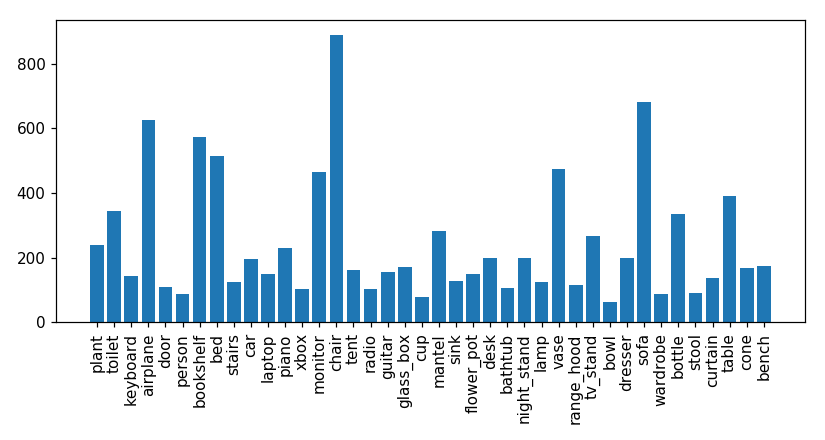
\includegraphics[width=\textwidth]{Figures/shape_retrieval/modelnet_classes.png}
    \caption{ModelNet40 data set: distribution of samples per class.}
    \label{fig:modelnet_classes}
\end{figure}

\subsection{Implementation details}
To demonstrate the impact that the triplet based training has on the performance of CNN descriptors
we use a deep network architecture shown in a Table~\ref{tab:net-architecture}. This network was implemented in PySparseConvNet, which is our modification of the SparseConvNet library \cite{graham2014spatially}. Besides new loss functions PySparseConvNet can be accessed from Python for a more interactive usage.

When forming a triplet for training we choose uniformly randomly a positive pair of objects from one class
and select a negative sample uniformly randomly from one of other classes.

For the optimization we use the SGD \cite{bottou-tricks-2012}, and the training is done
\begin{itemize}
\item in batches of size from $45$ to $90$ depending on a GPU video memory,
\item with a learning rate of $0.002$,
\item and a momentum equal to $0.99$.
\end{itemize}
Training can take up to a week on a server with advanced GPU, such as NVIDIA Titan X or GTX980ti.

\begin{figure}
\centering
\begin{tabular}{ccccc}
  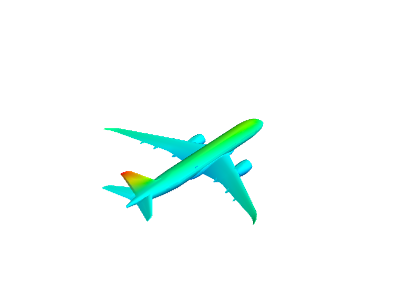
\includegraphics[width=0.19\columnwidth]{Figures/shape_retrieval/pic_airplane_solid.png} &
  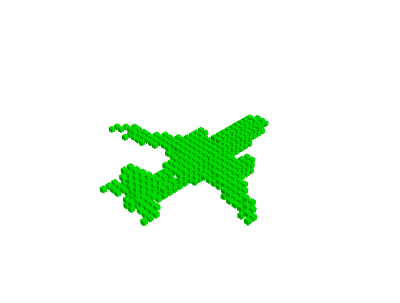
\includegraphics[width=0.19\columnwidth]{Figures/shape_retrieval/pic_airplane_30_solid.png} &
  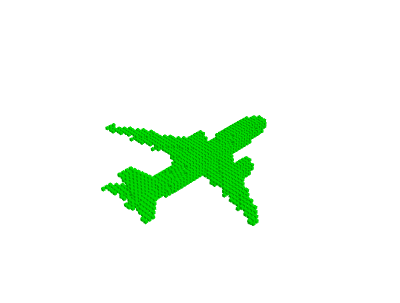
\includegraphics[width=0.19\columnwidth]{Figures/shape_retrieval/pic_airplane_50_solid.png} &
  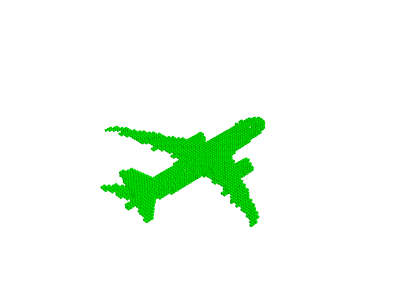
\includegraphics[width=0.19\columnwidth]{Figures/shape_retrieval/pic_airplane_70_solid.png} &
  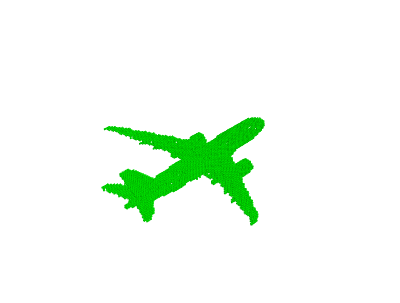
\includegraphics[width=0.19\columnwidth]{Figures/shape_retrieval/pic_airplane_100_solid.png} \\
% (a) first & (b) second \\
 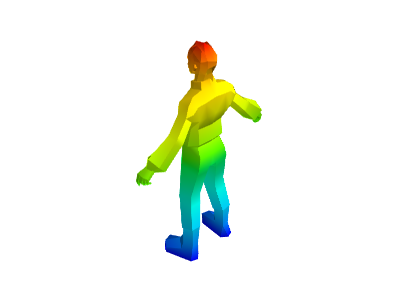
\includegraphics[width=0.19\columnwidth]{Figures/shape_retrieval/pic_person_solid.png} &
 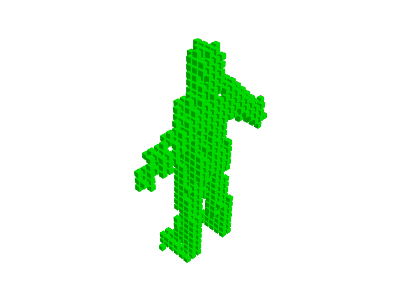
\includegraphics[width=0.19\columnwidth]{Figures/shape_retrieval/pic_person_30_solid.png} &
 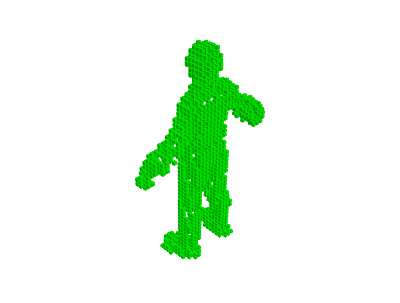
\includegraphics[width=0.19\columnwidth]{Figures/shape_retrieval/pic_person_50_solid.png} &
 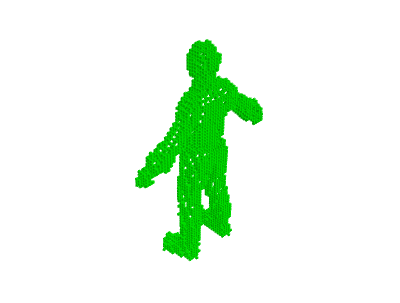
\includegraphics[width=0.19\columnwidth]{Figures/shape_retrieval/pic_person_70_solid.png} &
 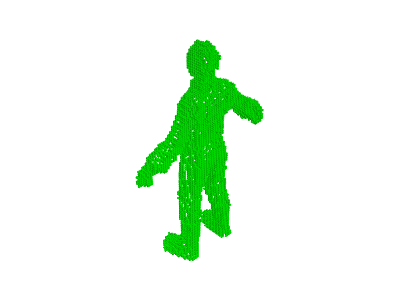
\includegraphics[width=0.19\columnwidth]{Figures/shape_retrieval/pic_person_100_solid.png} \\

 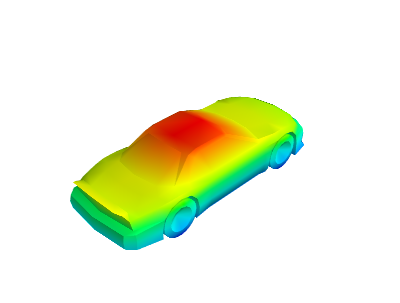
\includegraphics[width=0.19\columnwidth]{Figures/shape_retrieval/pic_car_solid.png} &
 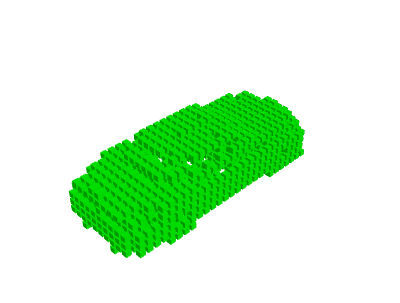
\includegraphics[width=0.19\columnwidth]{Figures/shape_retrieval/pic_car_30_solid.png} &
 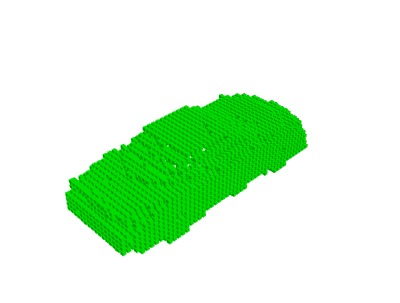
\includegraphics[width=0.19\columnwidth]{Figures/shape_retrieval/pic_car_50_solid.png} &
 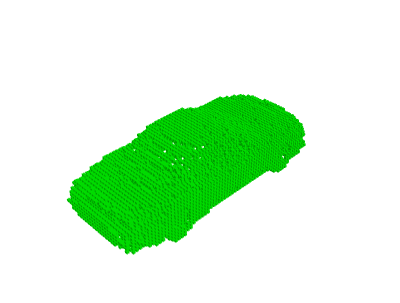
\includegraphics[width=0.19\columnwidth]{Figures/shape_retrieval/pic_car_70_solid.png} &
 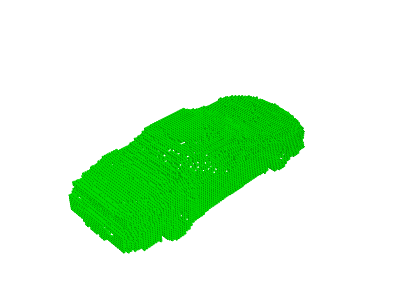
\includegraphics[width=0.19\columnwidth]{Figures/shape_retrieval/pic_car_100_solid.png} \\
\end{tabular}
\caption{Examples of some objects voxelizations at different resolutions $30$, $50$, $70$, $100$ (from left to right), left-most objects are depicted using original meshes}
\label{fig:voxels-examples}
\end{figure}


We train Sparse 3D Convolutional Neural Network (S3DCNN) on the 3D shape classification dataset by splitting it into  training and validation subsets, adding augmentation of data to achieve rotational and translational invariance. After training a model on a dataset of pairs, we use it to embed voxel representations of 3D meshes into $192$-dimensional space. The retrieval consist of ranking search objects by a cosine distance of vectors from a query vector.

The most popular metrics for evaluating retrieval performance are
\begin{itemize}
\item Precision-Recall Curve shows a trade-off between these two measures and how quickly the precision drops with the recall increase,
\item Mean average precision (mAP). Given a query, its average precision is the average of all precision values computed on all relevant objects in the retrieved list. Given several queries, the mean average precision (mAP) is the mean of average precisions for these queries. 
\end{itemize}
We evaluated mAP for different voxel rendering sizes of 3D shapes both at train and test times, see also Figure~\ref{fig:voxels-examples}.

To check if our model is comparable with other architectures, we consider a classification task. So, we trained our model for the classification task using the ModelNet40 train subset with 
\begin{itemize}
\item SoftMax last layer for $200$ epochs,
\item with exponentially discounting learning rate,
\item and performed retrieval evaluation on the test subset,
\item taking $20$ images from every class, and ranking them w.r.t their $L2$-norm by activations taken from the $17$-th layer.
\end{itemize}

Results of these experiments are provided in Table~\ref{tab:classification}. We can see that in case of classification task setup our model is comparable in terms of the classification accuracy, but mAP values are worse. But in case of metric learning performace of S3DCNN on mAP metric is much better.
Superior performance of retrieval task with MVCNN is not a surprising result, since MVCNN uses neural nets, pre-trained on ImageNet. On the other hand our model only requires 3D Shape dataset to learn.

In Figure~\ref{fig:map_for_rs} we provide the dependence of mAP on the input spatial resolution. We can see that the retrieval performance improves with increase in the input spatial resolution up to around $45-50$, after that it drops slightly and goes to plateau. It can be attributed to the insufficient amount of layers for the same scale of features, that can be separated in higher layers. Light blue color shows range of mAP on validation for top $30$ trained architectures.


\begin{figure}[!tbp]
\vspace{-20pt}
\centering
\begin{minipage}[b]{0.45\textwidth}
  \centering
  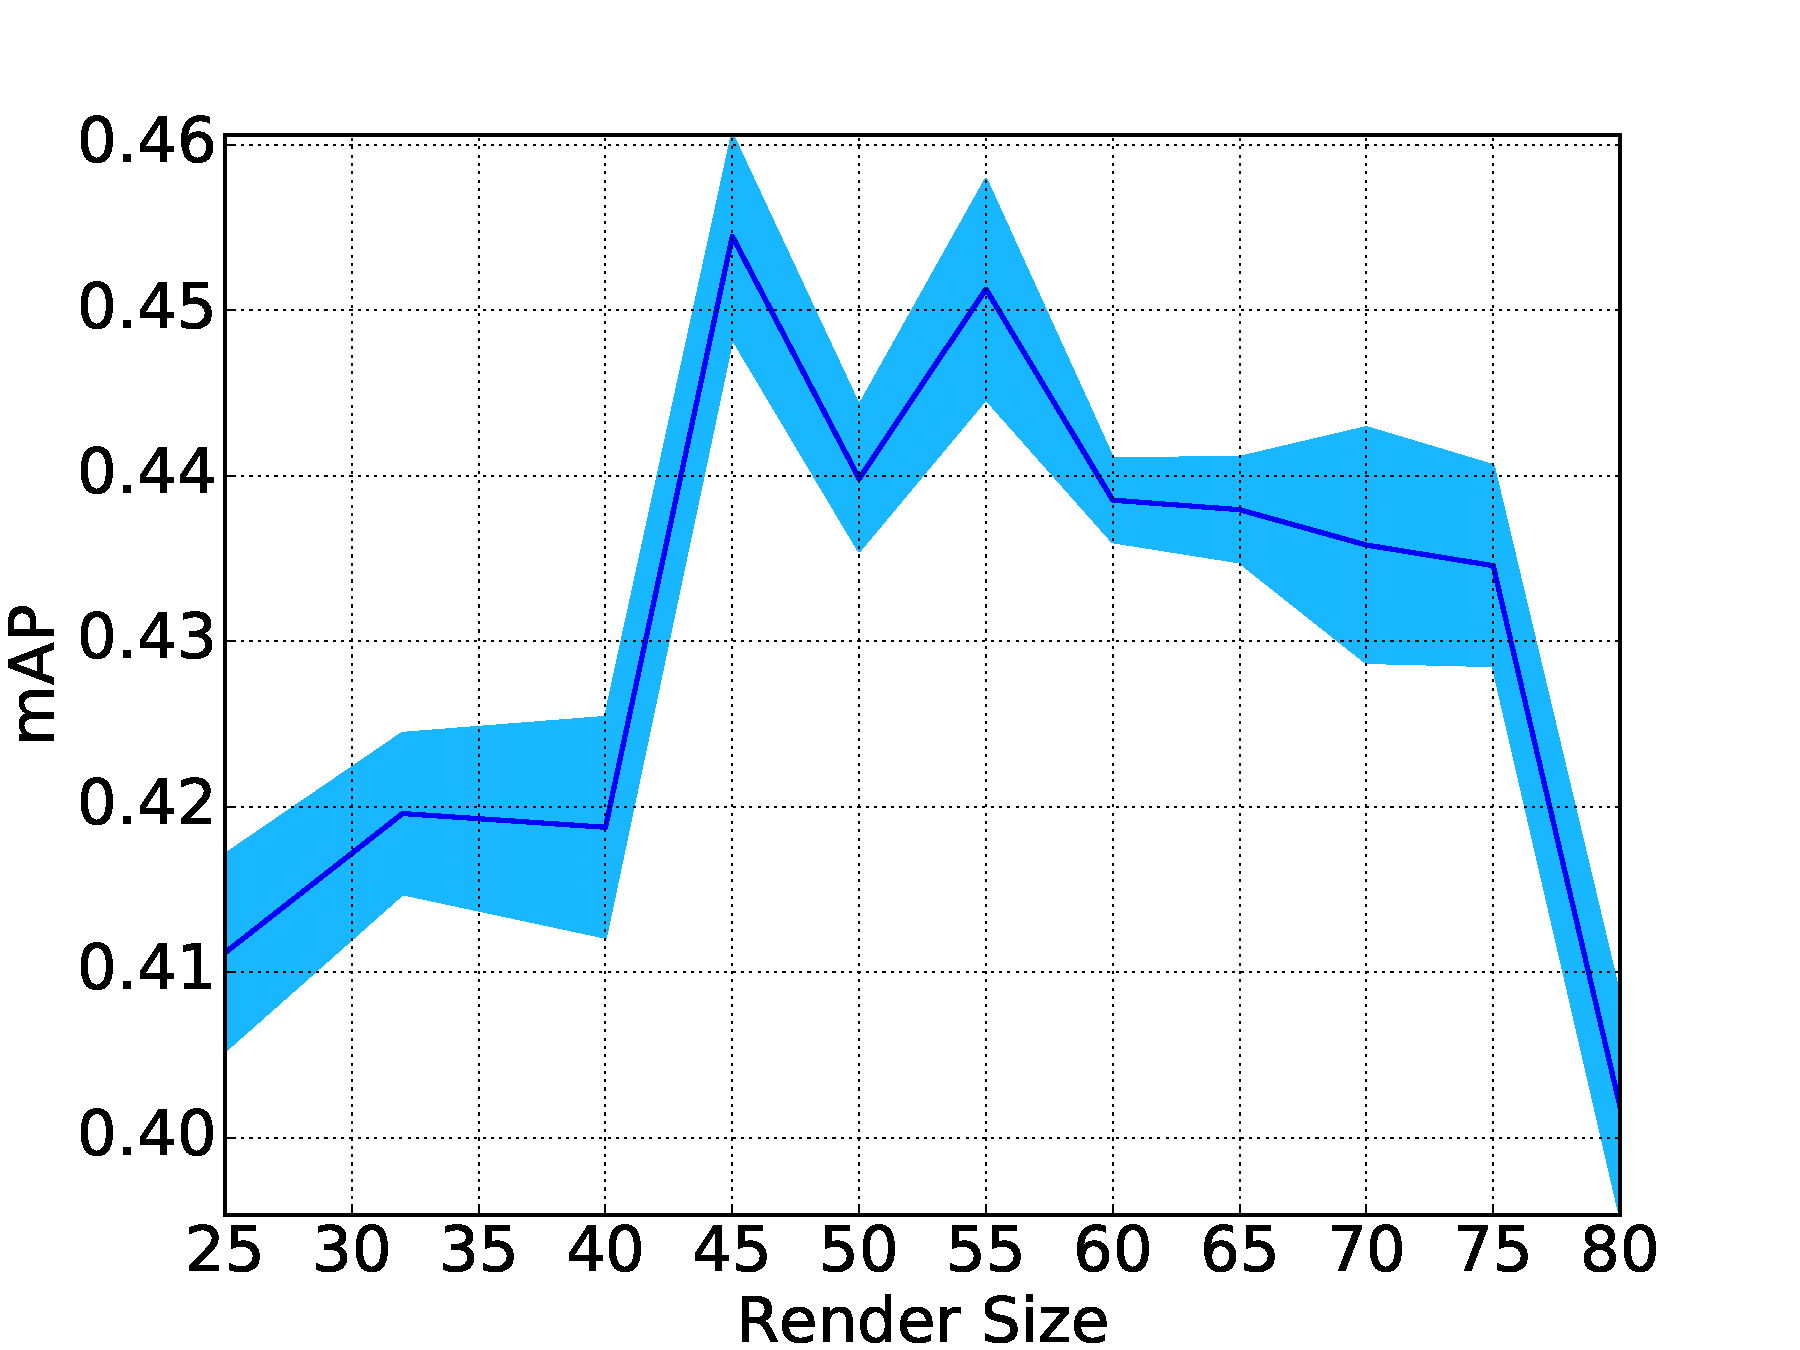
\includegraphics[width=\columnwidth]{Figures/shape_retrieval/new_map_to_rs.pdf}
  \caption{Dependence of the retrieval performance on the input spatial resolution}
  \label{fig:map_for_rs}
\end{minipage}
\begin{minipage}[b]{0.45\textwidth}
  \centering
  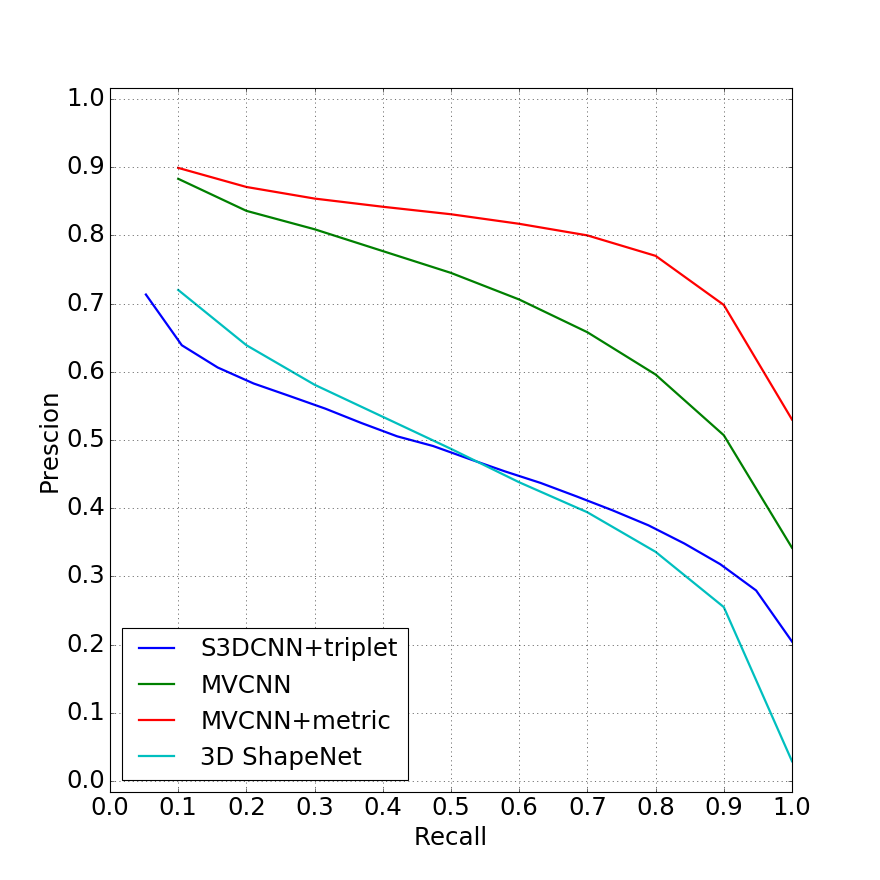
\includegraphics[width=\columnwidth]{Figures/shape_retrieval/pr_curves_comp}
  \caption{Precision-Recall curve for our method}
  \label{fig:pr_curve}
\end{minipage}
\end{figure}


We would like to note that in Figure~\ref{fig:map_for_rs} mAP values provided for different validation epochs and variability of best model can be explained by difference in total learning time.

% \begin{itemize}
% \item In Table~\ref{tab:classification} for the retrieval we used features from the last but one layer of the network,
% \item In Figure~\ref{fig:map_for_rs} we used learning with the triplet loss, for which we still have to better adjust the architecture and learning rate schedule.
% \end{itemize}


\section{Results}
\label{sec:5}

\begin{figure}
  \centering
    \includegraphics[width=\textwidth]{Figures/shape_retrieval/cnn_embed_2k.jpg}
    \caption{t-SNE plot of ModelNet40 validation set}
    \label{fig:modelnet_tsne}
\end{figure}

We found that the retrieval performance improves with increase in the input spatial resolution. However, such an effect is difficult to check experimentally and to use in practice, as e.g. for usual 3D dense CNNs the computational time is prohibitively large. In our case, data sparsity helps us to process data in reasonable time even with input resolution up to $100^3$ voxels, therefore we can benefit from the increase of the input spatial resolution when performing retrieval.
In Figure~\ref{fig:pr_curve} we can see that our method is comparable to \cite{wu20153d} in low recall, and better at higher recall values, that indicates better scalability of our method.
In Table~\ref{tab:classification} for the retrieval we used features from the one before last layer of the network of size 192, which in  comparison to 4000 in 3DShapeNet model \cite{wu20153d} is 20 times smaller but achieves almost the same retrieval metrics.


We evaluated our network architecture described in Table~\ref{tab:net-architecture} on popular state-of-the-art frameworks for Deep Learning, such as Tensorflow~\cite{tensorflow2015-whitepaper} on GPU and \cite{2016arXiv160502688short} on CPU.
Using Keras \cite{chollet2015keras} 2.0.2 with Tensorflow~\cite{tensorflow2015-whitepaper} 1.2.1 backend on Nvidia Titan X GPU with 12Gb of GPU memory, we were able to exhaust all of it with batch size equal to 12, and performed forward passes on average 0.0301 seconds/sample, which is comparable to processing speed of our implementation with render size of about 60-70.
Other setup was an implementation of our network architecture on Keras with Theano backend using Intel i7-5820K 6-core CPU processor, took 1.53 seconds/sample, which is significantly slower.
% We provide training code for all experiments in our repository\footnote{\url{https://github.com/gangiman/PySparseConvNet}}.


\begin{table}[t]
  \caption{Evaluation on Modelnet40}
  \label{tab:classification}
  \centering
  \begin{tabular}{llll}
    \toprule
    method & Classification & Retrieval AUC & Retrieval mAP \\
    \midrule
    3DShapeNet \cite{wu20153d} & 77.32\% & 49.94\% & 49.23\% \\
    MVCNN \cite{su15mvcnn} & 90.10\% & --- & 80.20\% \\
    VoxNet \cite{maturana2015voxnet} & 83.00\% & --- & --- \\
    VRN \cite{brock2016generative} & 91.33\% & --- & --- \\
    \textbf{S3DCNN (proposed)} & \textbf{90.30}\% & \textbf{36.05}\% & \textbf{33.67}\% \\
    \textbf{S3DCNN + triplet (proposed)} & --- & \textbf{48.81}\% & \textbf{46.71}\% \\
    \bottomrule
  \end{tabular}
\end{table}

\subsubsection*{Acknowledgments}
We are very grateful to Dmitry Yarotsky for his contribution to this research project. Big Thanks to Benjamin Graham for some useful comments and ideas. Thanks to Rasim Akhunzyanov for his help in debugging the PySparseConvNet code.

The research was partially supported by the Russian Science Foundation grant (project 14-50-00150).

% \clearpage
% \bibliographystyle{abbrv}
% \bibliography{bibliography}

% \end{document}

\newpage 
% 


\chapter{Multi-region Bilinear Convolutional Neural Networks for Person Re-Identification}

\label{chapt:bilinear}

\section{Motivation}
%: relation to fine-grained recognition and Bilinear CNNs
%TODO relocate images (false positive-left, )
\begin{figure*}[t]%{R}{0.5\textwidth}
\centering

\begin{tabular}{c c}

    False positives & False negatives \\
    \begin{tabular}{c c }
    % 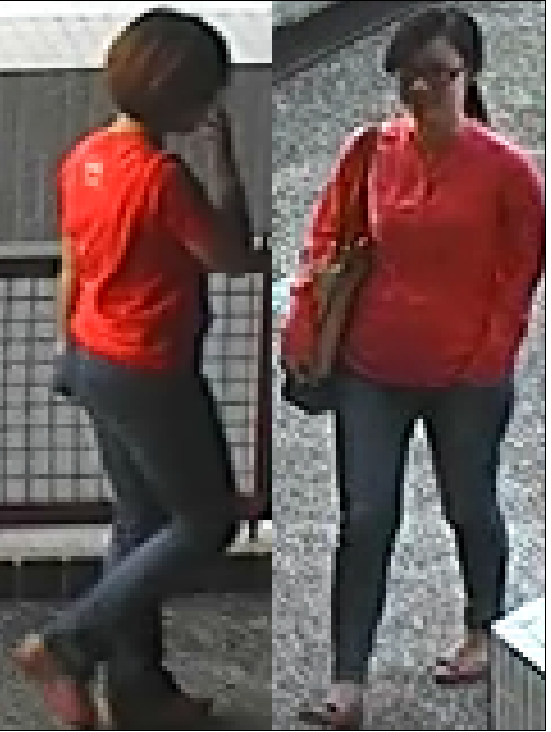
\includegraphics[ height=3.5cm, width=2.5cm]{\bilinearroot/figures/pedestrians_pairs/false_pos1.png}&
    % 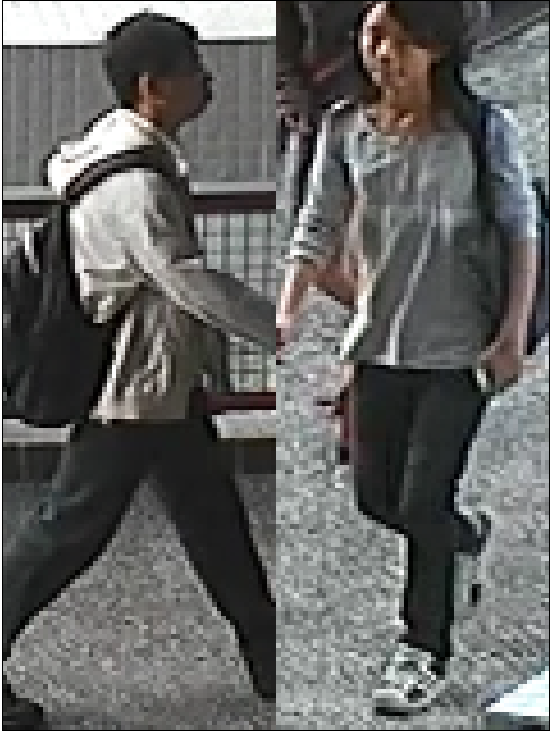
\includegraphics[ height=3.5cm, width=2.5cm]{\bilinearroot/figures/pedestrians_pairs/false_pos2.png}\\
    % 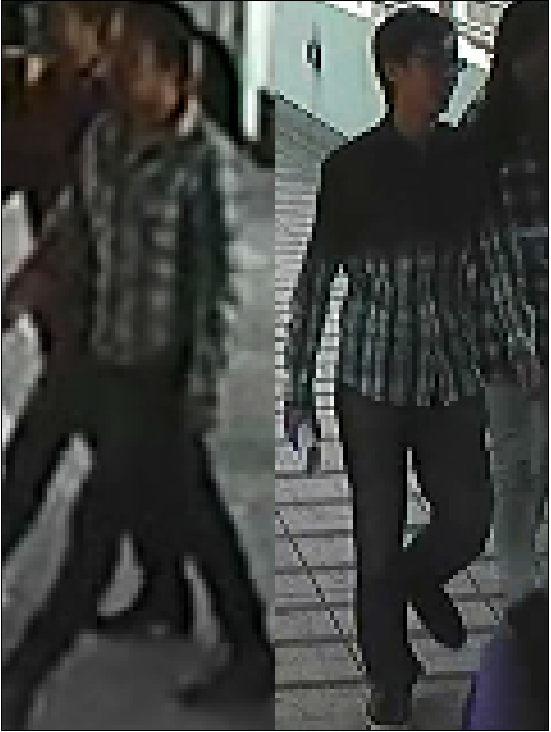
\includegraphics[ height=3.5cm, width=2.5cm]{\bilinearroot/figures/pedestrians_pairs/false_pos3.png}&
    % 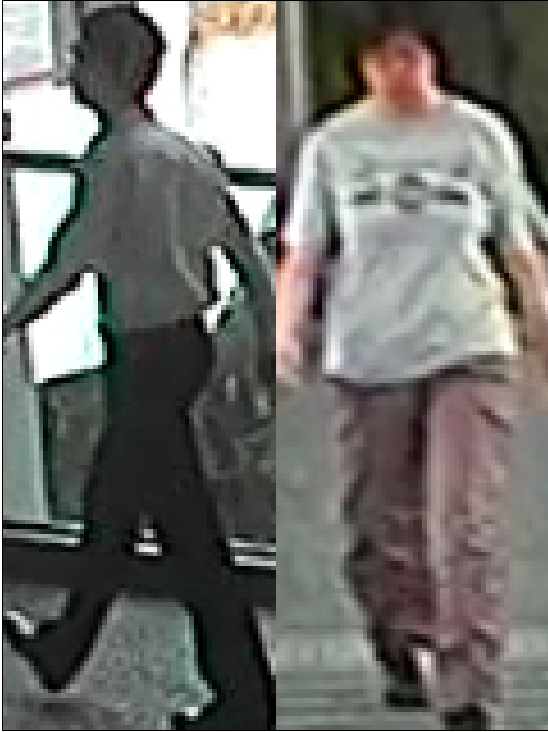
\includegraphics[ height=3.5cm, width=2.5cm]{\bilinearroot/figures/pedestrians_pairs/false_pos4.png}
    
    
    \end{tabular} &
    
    
    \begin{tabular}{c c }

    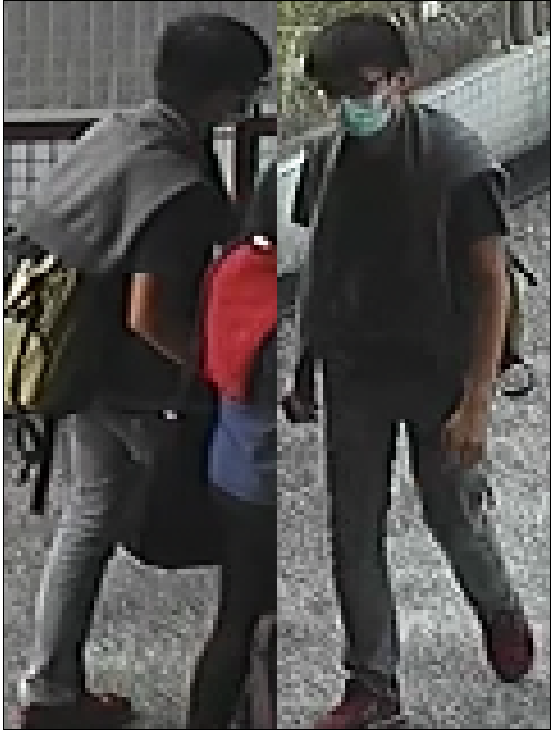
\includegraphics[ height=3.5cm, width=2.5cm]{\bilinearroot/figures/pedestrians_pairs/false_neg1.png}&
    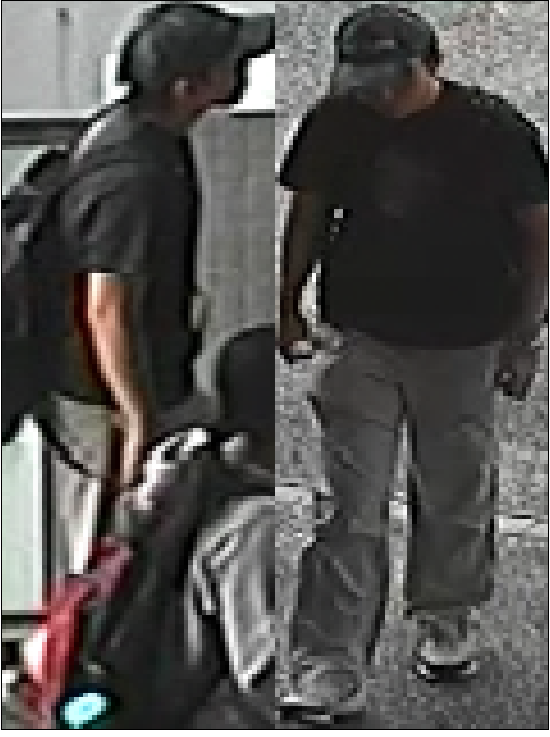
\includegraphics[ height=3.5cm, width=2.5cm]{\bilinearroot/figures/pedestrians_pairs/false_neg2.png}\\
    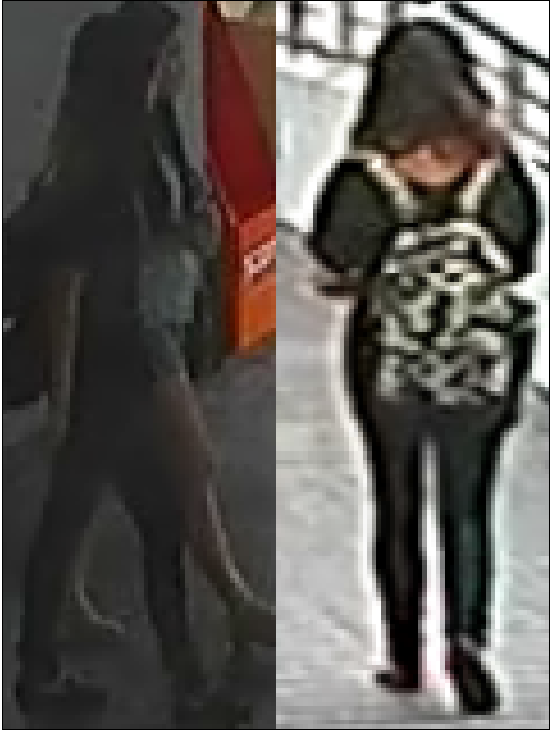
\includegraphics[ height=3.5cm, width=2.5cm]{\bilinearroot/figures/pedestrians_pairs/false_neg3.png}&
    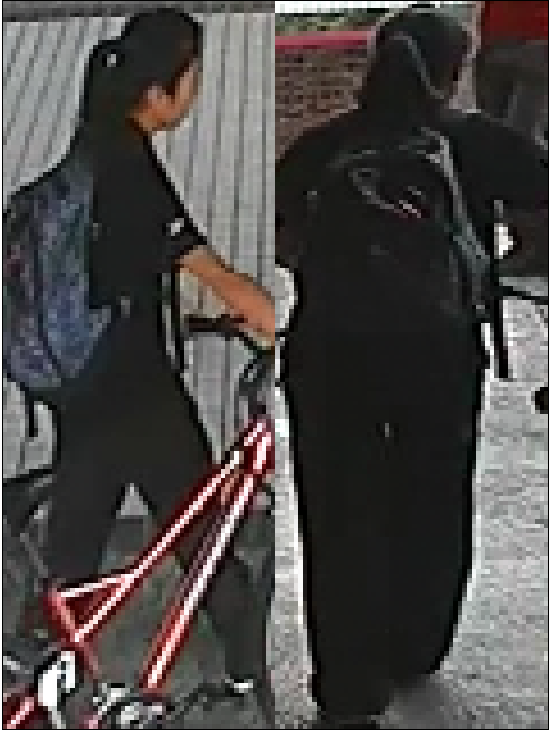
\includegraphics[ height=3.5cm, width=2.5cm]{\bilinearroot/figures/pedestrians_pairs/false_neg4.png}
    
    
    \end{tabular}
    \\

    
    \begin{tabular}{c }
    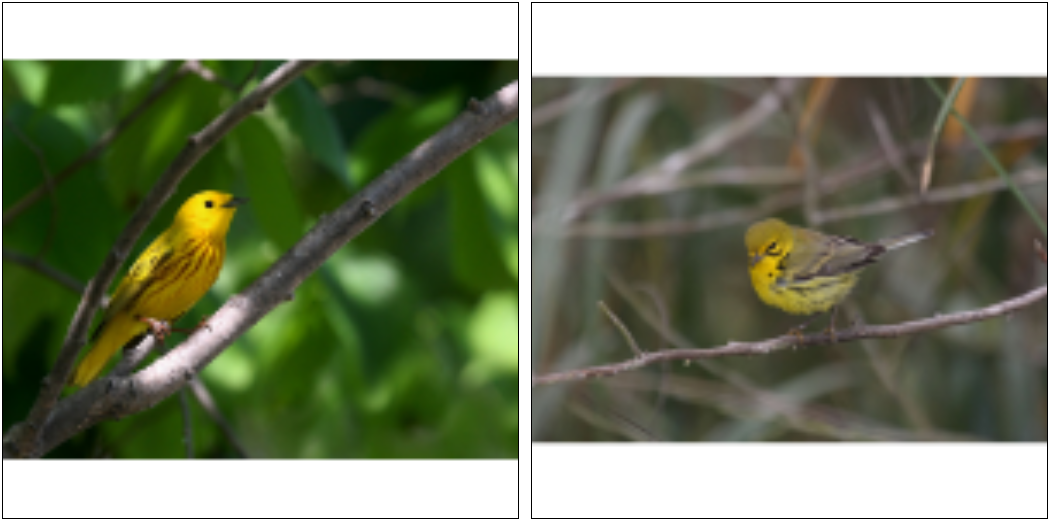
\includegraphics[ height=3cm, width=5.5cm]{\bilinearroot/figures/birds/birds_false_pos1.png}\\
    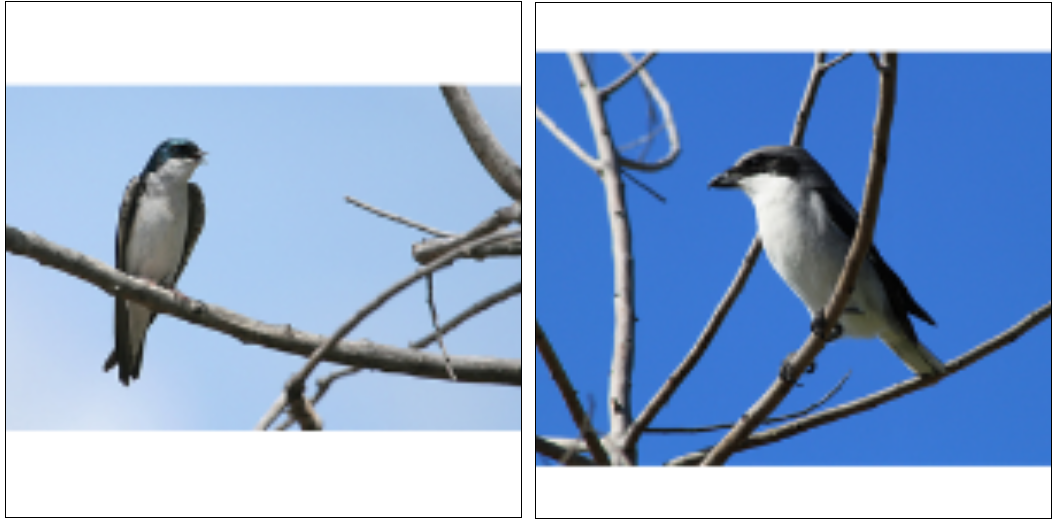
\includegraphics[ height=3cm, width=5.2cm]{\bilinearroot/figures/birds/birds_false_pos2.png}
    
    \end{tabular} &
    \begin{tabular}{c }

    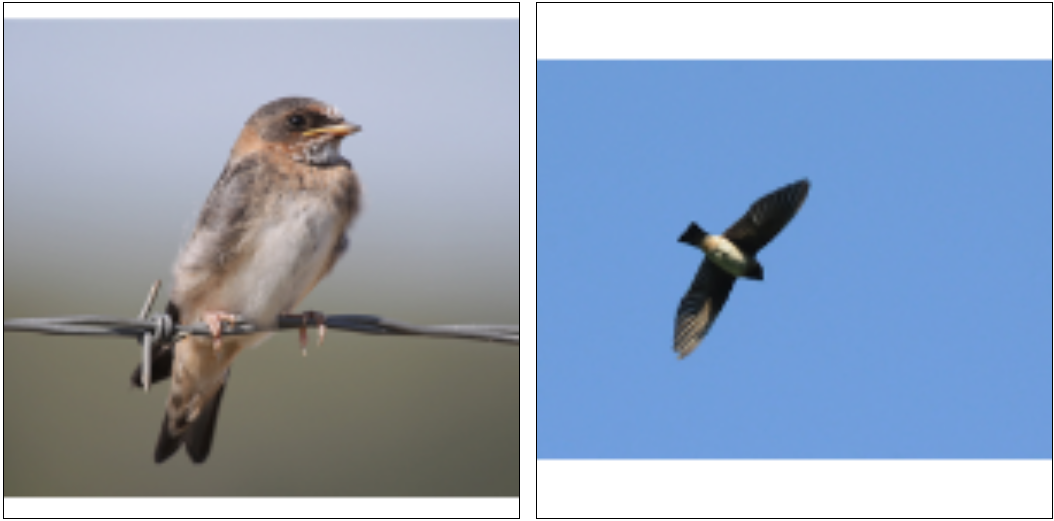
\includegraphics[ height=3cm, width=5.5cm]{\bilinearroot/figures/birds/birds_false_neg1.png}\\
    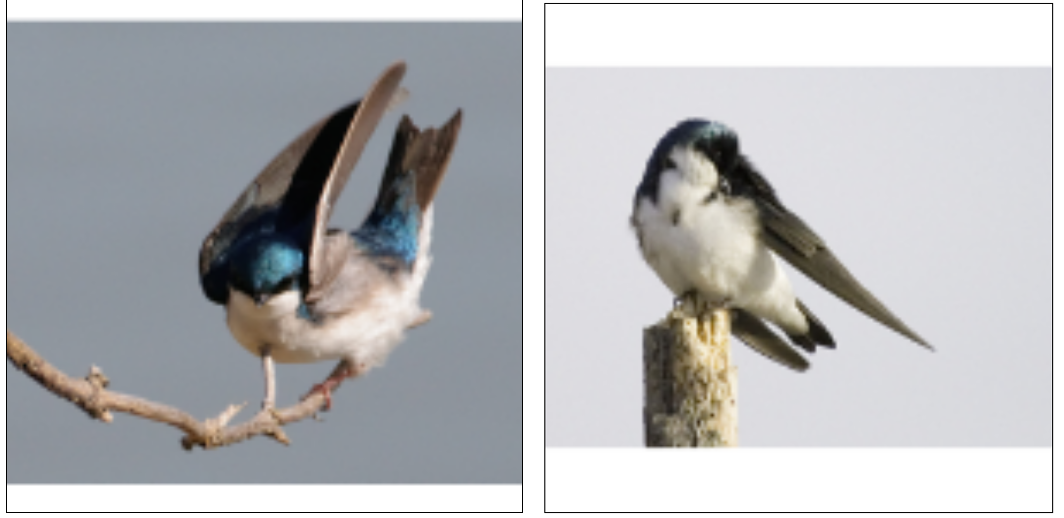
\includegraphics[ height=3cm, width=5.5cm]{\bilinearroot/figures/birds/birds_false_neg2.png}
    
    \end{tabular} 
    \\
    (a) & (b)


\end{tabular} 
\caption{Difficult re-identification cases in the CUHK03 dataset and the CUB-Birds dataset for the fine-grained classification~\citep{Wah11}. (a) -- the pairs of very similar images depicting different persons/bids species (b) -- the pairs of dissimilar images depicting the same person/bird species. There is a clear similarity between the challenges posed by the two tasks. Both re-identification and fine-grained classification deal with strong viewpoint variations, and often need to focus on small-scale fragments in order to distinguish subjects/classes. At the same time the re-identification task has a greater degree of alignment, and we therefore suggest a modification of the bilinear CNN exploiting the presenсe of such weak alignment in the re-identification case.}
\label{fig:teaser}
\end{figure*}

\textit{Fine-grained recognition tasks} are usually characterized by small visual differences between the categories and possibly large intra-category differences. The examples of the former are different bird species of similar color and pedestrians wearing similar clothes, the latter is often due to high variations caused by such factors as pose and lighting. 

The task of person re-identification shares considerable similarity with fine-grained categorization (see the example pairs in \fig{teaser}), as the matching process in both cases often needs to resort to the analysis of fine texture details and parts that are hard to localize. 

\textit{Bilinear convolutional neural networks} have been first suggested by \citep{lin2015bilinear} for fine-grained categorization tasks. The idea of this architecture is to utilize multiplicative interactions between different features computed using two feature extractor subnetworks. The intuition behind this suggests that such factorization may allow the model to learn such functions as detection (some parts may be detected, \eg{} birds beaks, heads) and recognition (\eg{} colors and textures). When the features carrying information about parts are combined in a  multiplicative way with the features carrying some texture information, the result may capture more complex concepts, \eg{} particular parts of particular color/texture.

The bilinear layer suggested by \citep{lin2015bilinear} is defined as follows:

\begin{equation}
   \label{eq:bilinear}
    x_{bilinear} = A^T B,
\end{equation}
where $A$ and $B$ are the outputs of the two deep feature extractors $f_A$ and $f_B$ (convolutional neural networks). $A \in \mathbb{R}^{S \times M}$, $B \in \mathbb{R}^{S \times N}$, $S$ is the number of spatial locations, $M$ and $N$ are the number of the featuremaps that the extractors $f_A$ and $f_B$ produce. The result of this operation is a matrix of size $M \times N$, but is reshaped to a vector $MN \times 1$.

Another characteristic that differs Bilinear CNNs from regular models is related to the way of handling the image spatial information. Non-bilinear architectures (\eg{} \citep{simonyan2014very}) apply fully-connected layers to the output of the last convolution layer to compute the final representation. In this case, each output element is computed by applying different weights to the input elements. It is easy to see that such operation may preserve some spatial information by assigning bigger weights for particular regions of the input feature maps. 

Bilinear CNNs, however, rather radically discard spatial information in the process of the sum-pooling. For very deep and powerful architectures like \citep{simonyan2014very}, such spatial information may be rather irrelevant and therefore can be easily discarded. In contrast, for more shallow architectures, like those that have been recently most popular for person re-identification, the radical pooling over all spatial locations may lead to a noticeable performance drop.

Moreover, as evidenced by the experiments of \citep{lin2015bilinear}, Bilinear CNNs with global pooling and powerful feature extractors are very appropriate for the tasks where pose variability may be very high, \eg{} bird species recognition  (for example of very different poses, see the lower picture in \fig{teaser}b). At the same time, the variability of geometric pose and viewpoints in re-identification problems is more restricted.

Thus the CNN architecture for person re-identification should be developed in the light of the discussed circumstances of this task, namely:
\begin{itemize}
    \item moderate-size architectures being used for person re-identification,
    \item more restricted pose variation of pedestrians, compared to other fine-grained recognition problems.
\end{itemize}
   
Given these preliminaries, it is appropriate to consider some intermediate variant that would preserve the features of both Bilinear and standard architectures. Indeed, such a variant, called Multi-region Bilinear CNN, is discussed later in this chapter. It can be regarded as a middle ground between the traditional CNNs and the Bilinear CNNs. In the experiments presented in this chapter, it is also shown that such a compromise achieves an optimal performance across a range of person re-identification benchmarks, while also performing favorably compared to the  previous state-of-the-art. The success of such architecture confirms the promise hold by deep architectures with multiplicative interactions such as Bilinear CNNs and the Multi-region Bilinear CNNs for hard pattern recognition tasks.

It should also be mentioned, that the Bilinear CNN with global pooling has been successfully applied to person re-identification by \citep{suh2018part} (after this work). The authors used powerful models of \citep{szegedy2015going} and \citep{cao2017realtime} (pre-trained for human pose estimation) for the recognition and detection streams correspondingly. This work presents some earlier (and lower) results, for which no explicit body part detection has been used. However, this work is the earliest to consider person re-identification a fine-grained problem and to adopt the Bilinear architecture for it. %discuss the results without pose estimation to our results?


%%%%%%%%% ABSTRACT
% \subsection{abstract}
% In this work we propose a new architecture for person re-identification. As the task of re-identification is inherently associated with embedding learning and non-rigid appearance description, our architecture is based on the deep bilinear convolutional network (Bilinear-CNN) that has been proposed recently for fine-grained classification of highly non-rigid objects. While the last stages of the original Bilinear-CNN architecture completely removes the geometric information from consideration by performing orderless pooling, we observe that a better embedding can be learned by performing bilinear pooling in a more local way, where each pooling is confined to a predefined region. Our architecture thus represents a compromise between traditional convolutional networks and bilinear CNNs and strikes a balance between rigid matching and completely ignoring spatial information.

% We perform the experimental validation of the new architecture on the three popular benchmark datasets (Market-1501, CUHK01, CUHK03), comparing it to baselines that include Bilinear-CNN as well as prior art. The new architecture outperforms the baseline on all three datasets, while performing better than state-of-the-art on two out of three. The code and the pretrained models of the approach can be found at \url{https://github.com/madkn/MultiregionBilinearCNN-ReId}.



%% !TEX root = ../Thesis_main.tex
\chapter{Introduction}

%video surveillance+
%person re-id+
% originates from Multi-Target Multi-Camera Tracking 
%open world / closed world+
%face : verification/identification
%common aspects: detection , processing, recognition
%deep learning

%retrieval
%fine-grained recognition
%adaptation

%datasets (cut from the papers) + table with reid dataset?
%architectures
%definitions?
%contribution - what is done
\section{Context}
\subsection{Problem of 3D reconstruction}

\subsection{Approaches for solving 3D Reconstruction problem}

Solutions for a reconstruction problem can be grouped in two major groups: 1) Geometric approach - when problem is represented as optimisation of scene state given constrains on projections of scene state to data, 2) Machine Learning approach - inverse model is optimisation.

If $X$ - is scene data, $z$ - is the state of the scene, and $g_i(z)$ - projection function of 3D scene $z$ state to perspective $i$, then to find an optimal 3D reconstruction, one solves this minimisation problem:
\begin{equation}
z_{rec} = \min_z\sum_i|X_i-g_i(z)|_2 .
\end{equation}

This approach only solves problem for once scene and does not provide any semantic information about it, only basic geometric information. 
The second approach is more modern and better fitted for machine learning applications, because instead of optimizing state of the scene, it's optimizes a model that performs computation from input data to some semantic (intrinsic) parameters, and can be described as following optimisation procedure:
\begin{equation}
\min_\theta\sum_i|X_i-g_i(f_\theta(\pi))|_2,\ \ \pi=I_\theta(\{X_i\}_i),\ \ z=f_\theta(\pi),
\end{equation}
where $\pi$ - are scene parameters, $f_\theta(\pi)$ - is a generative model that generates 3D state $z$ and it's function is determined by tunable parameters $\theta$.

In reconstruction process information can be introduced in two possible ways: 1) input signal - data measured by some spatial sensor, 2) by adding a priori knowledge while training the Inverse model or by design choice of reconstruction algprithm. Between the two source exist a fundamental trade-off and detirmination of which is dominant can be quite difficult \cite{tatarchenko2019single}.


\subsection{Objectives and Motivations}

The goal of this work to improve methods of 3D reconstruction in holistic context using deep learning systems. For efficient applications such as robotics in human environments and mixed reality more advanced machine perception systems are needed. Human perception is a complex system with several properties not all of which are replicated in modern machine perception systems. From cognitive sciences it's known that ability to model environments is one of the most important for perception system, in area of computer vision this is known as an ability to perform \textit{3D reconstruction} of scenes and environments. To solve this problem in a general case requires application of machine learning.

In particular, the development of such holistic deep 3D reconstruction system includes several important tasks:

\begin{itemize}
􏰀    \item Capturing scenes, complete with colour and depth data of a sufficient quality,
    \item Recalling objects from large scale database of objects,
    \item Segmenting variety of most common elements from sensor data, such as household objects and architectural components,
    \item Detecting and reconstructing shape and pose of and human bodies.
\end{itemize}

Each of these sub-tasks constitutes a challenge in the context of human perception.

The presence of noise in sensor data (e.g., consumer grade depth cameras) is a serious problem for all downstream sub-tasks, low fidelity of this data causes a considerable compaunding performance drop.

\subsection{3D data representations}

We can describe a 3D object in multiple ways, and codification of it's properties has ramifications about capturing different information about objects and scenes, as well as kinds of models that can regenerate them or computational resources needed to process it.
Each representation has it's own pros and cons. We assume 3D information representation to be positive effective and usefull if it captures more relevant information with less storage requirement (compression), increases signal to noise ratio of data, captures shape and texture properties with minimum trade-off.

Here are some popular examples of 3D data representations:
\begin{enumerate}
	\item Multiple 2D projections - captures surface texture, highly redundant representation if images overlap, also vulnerable to optic illusions.
	\item Voxels - simple, most of the time can be sparse, represents rough volumetric properties vell but losses most of surface properties.
	\item Point Cloud - are sparse in a sense that they don't capture empty space, losing all surface properties besides color and estimated normals and most of volumetric properties.
	\item 2.5D (RGB-D) images are widespread because of cheap measurement devices, capture volumentric depth but succeptable to occlusion of bodies in a scene and records a lot of noise with actual signal.
\end{enumerate}



%Motivation: RGB-D scanning is here and we want to have a fine-grained understanding of the 3D captures
In the recent years, a wide variety of consumer-grade RGB-D sensors, such as the Intel Real Sense, Microsoft Kinect, depth-sensor enabled smartphones, enabled inexpensive and rapid RGB-D data acquisition. Increasing availability of large, labeled datasets (e.g.,~\cite{chang2017matterport3d,dai2017scannet})  made possible development of deep learning methods for 3D object classification and semantic segmentation. At the same time, acquired 3D data is often incomplete and noisy; while one can identify and segment the objects in the scene, reconstructing high-quality geometry of objects remains a challenging problem.  

An example of the new approach in recent work 
\cite{avetisyan2019scan2cad}, uses a large dataset of clean, labeled geometric shapes
\cite{chang2015shapenet}, for classification/segmentation associating the input point or voxel data with object labels from the dataset, along with adapting geometry to 3D data.  This approach ensures that the output geometry has high quality, and is robust with respect to noise and missing data in the input.  
At the same time, a ``flat'' classification/segmentation approach, with each object in the database corresponding to a separate label and matched to a subpart of the input data corresponding to the whole object, does not scale well as the number of classes grows and often runs into difficulties in the cases of extreme occlusion (only a relatively small part of an object is visible). 
Significant improvements can be achieved by considering object \emph{parts}, or more generally part hierarchies. 
Part-based segmentation of 3D datasets promises to offer a significant improvement both in finding the best matching shape in the dataset, recognizing objects from  highly incomplete data (e.g., from a couple of parts) from  as well as more precise geometry adaptation as well as, potentially, assembly of new shapes out of existing parts yielding a closer match to the input data. 

large collection of 3D models in database can be reduced to structured representations, 
objects with occluded sub-parts still can be recognized by parts available in the scan and the rest can be guessed with high probability, using parts, we can reconstruct new objects that are not yet present in the database of shapes.

Based on different approaches for volumetric information integration, from enhancements of  methods such as volumetric fusion \cite{curless1996volumetric}, to probabilistic  methods, and plethora of methods based on their combinations.

Compared to computer graphics models manually created by 3D professionals, 3D scans are noisy and incomplete.
Amount of noise and limited resolution of consumer-grade scanning hardware pose significant challenges for solving this important problem of scene reconstruction. 
Approaches of reconstruction based on fitting existing 3D assets into scene scans, have shown a lot of promise but still had problems with finding exact models from large database such as ShapeNet \cite{chang2015shapenet}, because of occlusion and lack of spatial context.

Learning-based approaches are very good at extracting features representative of objects and scenes as a whole, allowing to fill in occluded areas or guess parts affected by noise \cite{dai2017shape,dai2018scancomplete,song2017semantic}. These features are sufficient for scene completion, but they are not as good at recovering geometric primitives like: sharp edges, planar surfaces or borders between sub-parts, resulting in reconstruction quality much poorer than that of 3D content created by humans.

In this work, we focus on the key problem of semantic part segmentation of objects in the scenes, enabling further improvements in  dataset-based reconstruction. 
Semantic part-segmentation, can help in these situations, when sufficient number of the object parts is visible model can infer the non-visible parts essentially completing an object in sense of maximum probability conditioned on input data.

In human-made environments, a lot of objects have naturally defined semantic sub-parts, and those sub-parts can, in turn, have their sub-parts, i.e., parts form \emph{hierarchies}.  In our work, we use scene and object representation based on such part hierarchies.  We show how a part-labeled dataset of scanned 3D data suitable for machine learning applications can be constructed, and used to improve the performance of segmentation algorithms. 

Definitions of sub-parts are based on a set of primitive elements that were manufactured by one formation method or from one material.

Because of that and the fact that static scenes have other relationships between objects (fixed to each other or in direct surface contact), it's reasonable to suggest a scene description format that possesses a property of hierarchy (e.g., trees or other kinds of graphs).
Representing scenes as a discrete structures with multiple relationships between nodes. Such relationships like composability of its parts and affordances between whole objects, in turn allowing to compose a scene from separate objects.

\todo{merge these paragraphs}

In domain of human-made environments a lot of objects have sub-parts and those sub-parts can in turn have their own sub-parts. Definition of sub-part is often based on a set of primitive elements that were manufactured by one formation method or from one material. Because of that and the fact that static scenes have other relationships between objects (fixed to each other or in direct surface contact), it's reasonable to suggest a scene description format that possess a property of hierarchy (e.g. trees or other subgraphs).
A lot of researchers over the last 20 years came to the same conclusion. A lot of work on that problem was done by Mumford and Zhu in \cite{zhu2006stochastic}.

One of the papers dealt with problem of modeling Images as a hierarchy of super-pixels. \cite{russell2009associative}, or as a tree of geometric primitives (e.g. cylinders, spheres or 3D boxes) \cite{li2017grass}.

% point cloud (PC) turned in to a graph (based on proximity) point-cloud parser network reduces number of nodes and edges and enriches their feature vectors. First part of the decoder network functions similar to Feature Pyramid Network in CNNs, which performs local computations on different scales, followed by "pooling or convolutions" with reduced spatial component and increased feature components, thus leaving only small number of "keypoints" required to outline shapes of objects.



CAD constructor network translates that graph into CAD object (tree with primitives and combination rules). CAD rendered makes a mesh out of that object thus a residual between original PC and Mesh can be calculated.

Proximity Graphs - concept that allows to build a bridge between Point Clouds and Graph Processing. This area of computational geometry has a lot of theoretical results to offer for Deep Learning piplene designer.


\subsection{Definitions and examples}
\subsection{Data sources and devices}

\section{Inverse Graphics Problem formulation}

\cite{rezende2016unsupervised,eslami2016attend,kulkarni2015deep,wu20153d,izadinia2017im2cad}

Inverse graphics approach enables to solve a problem of "real-world" scene understanding through reconstruction of that scene and comparison it to measured data in some form.

Because it's a fairly new method it has some unexplored facets:
\begin{enumerate}
    \item How can we scale to hundreds and thousands of objects with different parameters.
    \item Embedded representations better than procedural generation
    \item Are there format that can have all advantages of CAD models and probabilistic properties that arise from real-world uncertainties.
\end{enumerate}

Central goals of computational perception is to get structured description of scenes from measurements such as photographic images, scans and videos.

Computer Vision as Inverse Graphics is the most rational formulations that could help us achieve this goal.

In the past, it has been hard to directly solve these problems in practice because of computational limitations.

However, it may be right time to take another look at this idea due to significant advances in deep learning for computer vision, probabilistic programming, and computer graphics.

Probabilistic programming - a tool that allows us to implement complex models while keeping ability to perform inference, extend with other probabilistic models by being general-purpose.

Re-formalizing inverse graphics in terms of probabilistic programming and deep learning allow us to solve even more complicated vision problems with off-the-shelf computational technology.

To make this approach scalable, my research can incorporate effective techniques such as: approximate Bayesian computation, differentiable programming for rendering.

Computer Graphics nowadays seems to be improving at a great pace in terms of designing solutions for hard image synthesis problems, but these solutions are usually hand-made and not flexible enough to cover all needs for general-purpose real world object generating, latest advances in generative models can help with that.


\subsection{Overcoming lack of information}

\section{Datasets}

Only recently research community started accumuulating sugnifficant amount of algined sensor data to solve large scale 3D reconstruction problems in deep learning context. In last 4 years we saw an explosion of 3D shape databases and 2D-to-3D indoor scene datasets, such as ShapeNet, 2D-3D Semantic, Scannet and Matterport3D datasets. Because accuracy and reacall properties of deep learning models scale with amount and variety of data, number of state-of-the-art models grew as well.

\section{Architectures}

PanopticFusion~\cite{narita2019panopticfusion} is a model that is able to segment large indoor scenes and separate \textit{Stuff} and \textit{Things}.


For outdoor datasets Point Cloud representation of data is more common because of large empty spaces and the way LiDAR sensor collects data. In such setting instance segmentation is nessesary first step for reconstruction~\cite{zhang2020instance}.

\subsection{Multi-view models}

Detailed comparision of multi-view 2D CNN model and 3D volumetric CNN can be found in \cite{qi2016volumetric}.

\subsection{Implicit 2D models}

Like inverse graphics network. Model takes 2D images and returns 2D images with 3D properties changed. 

\subsection{3D convolutional models}

Model generates or processes voxel image with 3D convolutional operation implemented Dense or Sparse.

Semantic information can boost the reconstruction performance because deep learning systems are able to pick up onto consistent signal \cite{jiao2018look,tatarchenko2019single,kendall2018multi}.

\subsection{2D to 3D Projection models}

Model uses camera parameters to compute 3D representation using 2D/2.5D images and projection operation.

\subsection{Point Set layers}

Neural Network processes a set of points to classify, segment or predict new set of points.

\subsection{Graph-Convolutional layers}

Model processes Geometric Graph where nodes represent points registered on a surface of objects or parts of objects, and has geometric or other information representing edges between points. Layers process activations associated with nodes taking into account the connectivity.

\subsection{Differentiable rendering layers}

Rendering operation is implemented in a differentiable way, allowing backpropogation of gradient information from 2D images to meshes and textures of the objects being rendered.

\subsection{Mesh generating layers}

Neaural Network layers that can create a mesh by way of processing a template 3D shape with parametracised operation or meshing other 3D shape representation generated by computation from weights and input.

\subsection{Implicit 3D models}

Models like NeRF, PIFU3D, neural network implements a rendering function depending on view angle and other graphics parameters, one model represents one scene and don't generalise for viriety of scene inputs.



\section{Contributions}

% \chapt{hist}, \chapt{bilinear} and \chapt{gradrev} use  person re-identification architecture of \citep{Yi14} as a baseline method (it is also  described in \sect{intro_architectures}).  \chapt{bilinear} is based on the results of \chapt{hist}: the loss function introduced in \chapt{hist} is used for 
% all the experiments in \chapt{bilinear} as it was demonstrated to show the best performance for person re-identification. 
% The results of \chapt{gradrev} were chronologically the earliest among all the results presented in this work, therefore  methods  from \chapt{hist} and \chapt{bilinear} were not used there. 
% Although the contributions of each of the chapters are independent, they are all parts of building a person re-identification pipeline and can be applied simultaneously. 
% \chapt{wildface} considers domain adaptation for surveillance face recognition and uses the method from \chapt{gradrev} as one of the baselines.
 




% \begin{figure*}[t]%{R}{0.5\textwidth}
% \centering

% \begin{tabular}{c c}

% \begin{tabular}{c c c c}

% 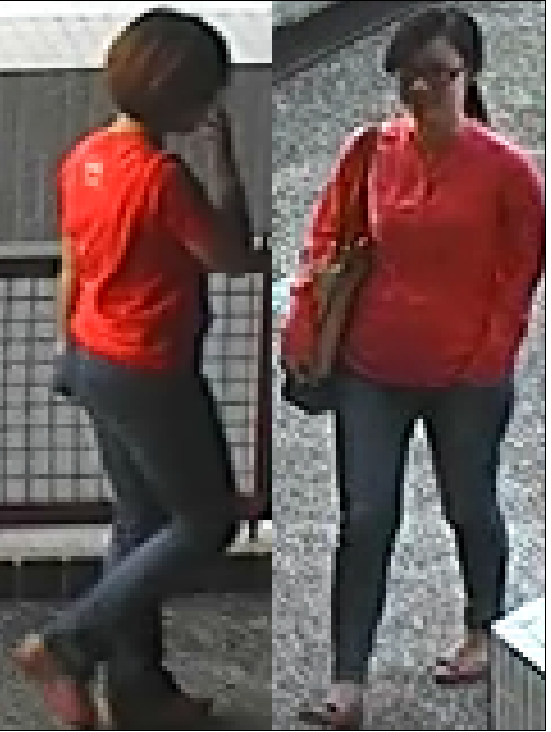
\includegraphics[ height=2cm, width=1.2cm]{\bilinearroot/figures/pedestrians_pairs/false_pos1.png}&
% 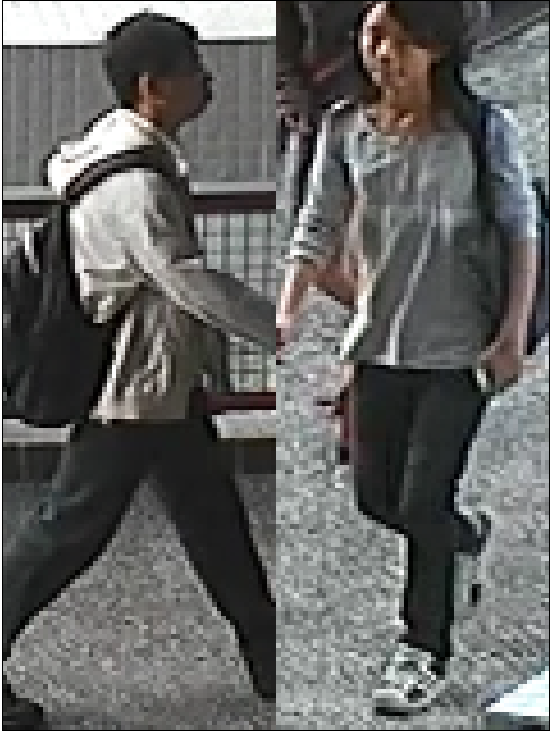
\includegraphics[ height=2cm, width=1.2cm]{\bilinearroot/figures/pedestrians_pairs/false_pos2.png}&
% 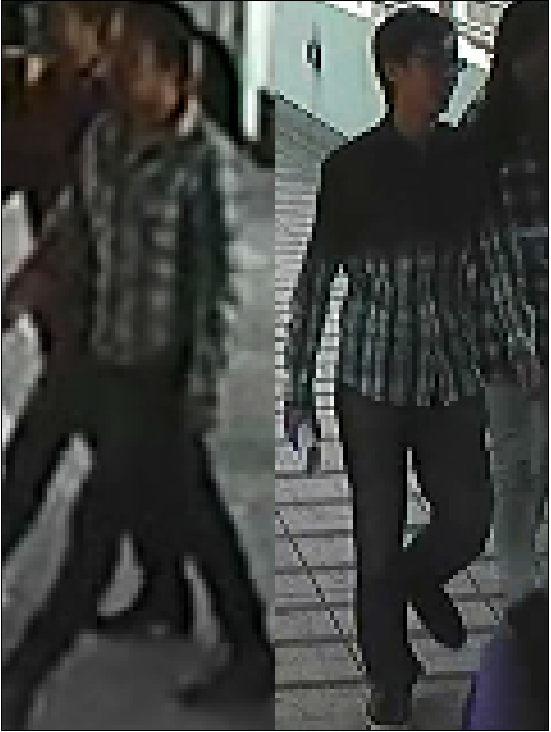
\includegraphics[ height=2cm, width=1.2cm]{\bilinearroot/figures/pedestrians_pairs/false_pos3.png}&
% 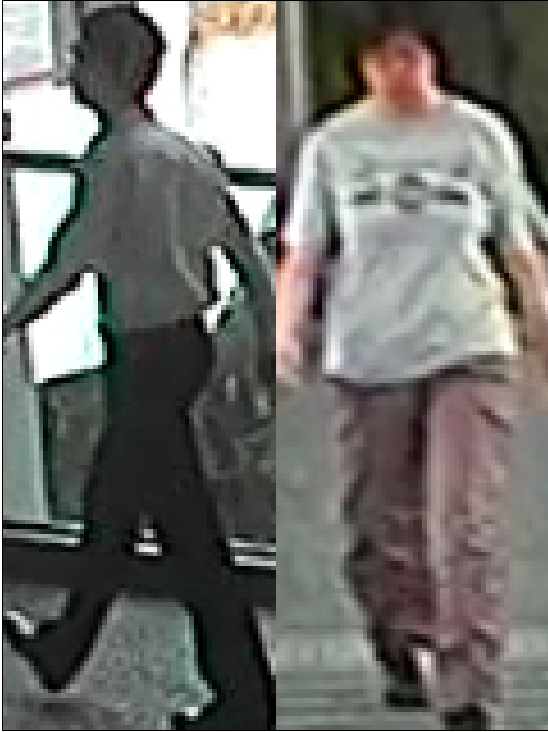
\includegraphics[ height=2cm, width=1.2cm]{\bilinearroot/figures/pedestrians_pairs/false_pos4.png}
% \\
% 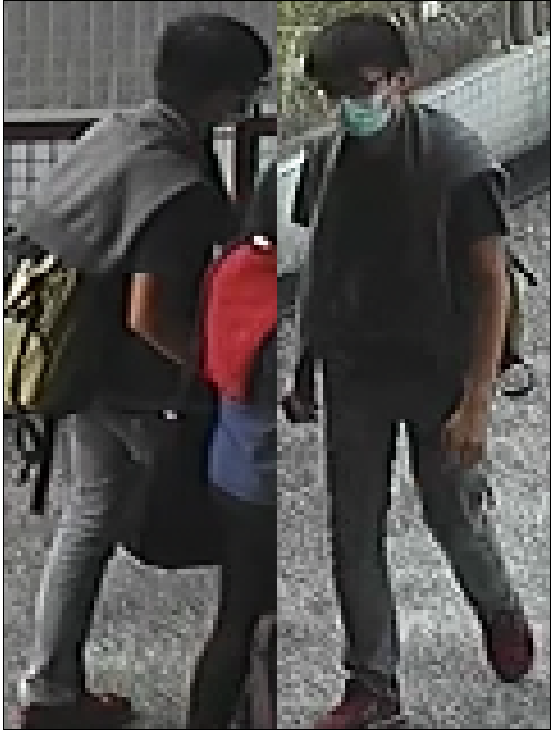
\includegraphics[ height=2cm, width=1.2cm]{\bilinearroot/figures/pedestrians_pairs/false_neg1.png}&
% 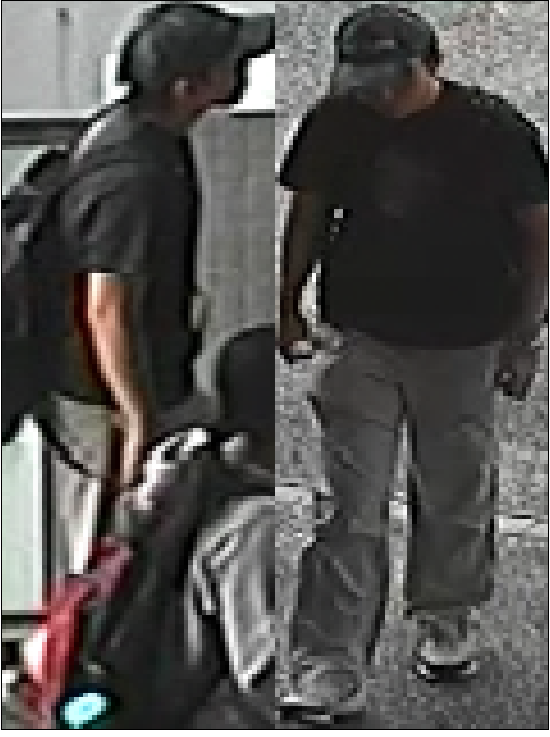
\includegraphics[ height=2cm, width=1.2cm]{\bilinearroot/figures/pedestrians_pairs/false_neg2.png}&
% 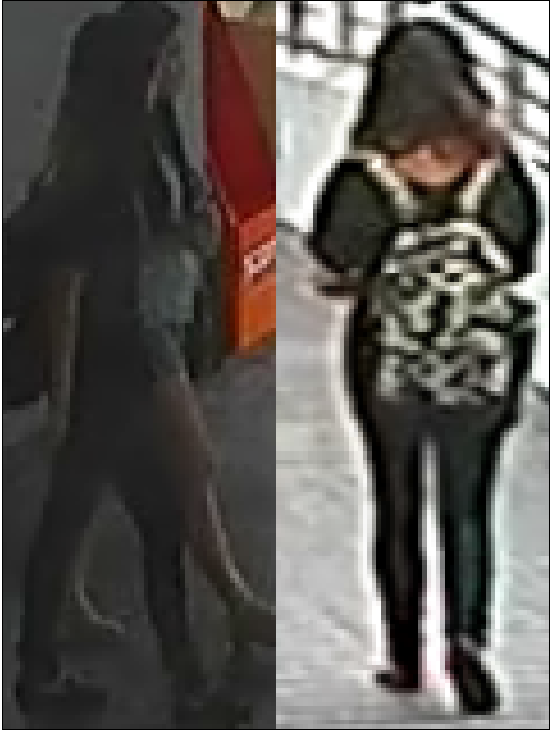
\includegraphics[ height=2cm, width=1.2cm]{\bilinearroot/figures/pedestrians_pairs/false_neg3.png}&
% 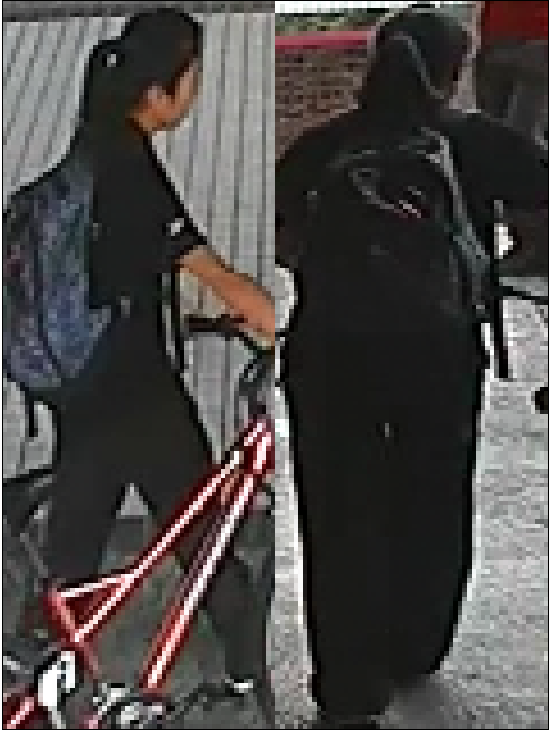
\includegraphics[ height=2cm, width=1.2cm]{\bilinearroot/figures/pedestrians_pairs/false_neg4.png}
% \end{tabular} &
% \begin{tabular}{c c}
% 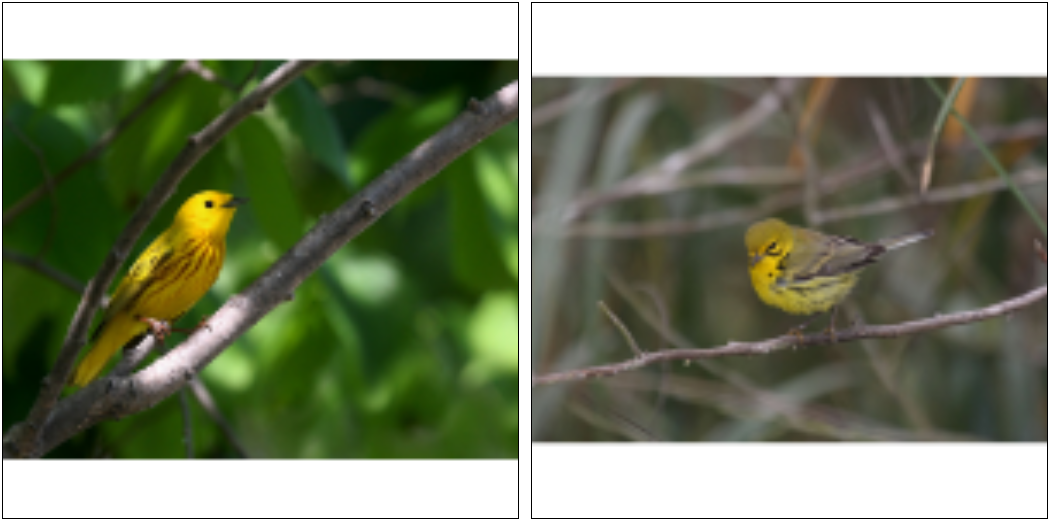
\includegraphics[ height=2cm, width=4cm]{\bilinearroot/figures/birds/birds_false_pos1.png}&
% 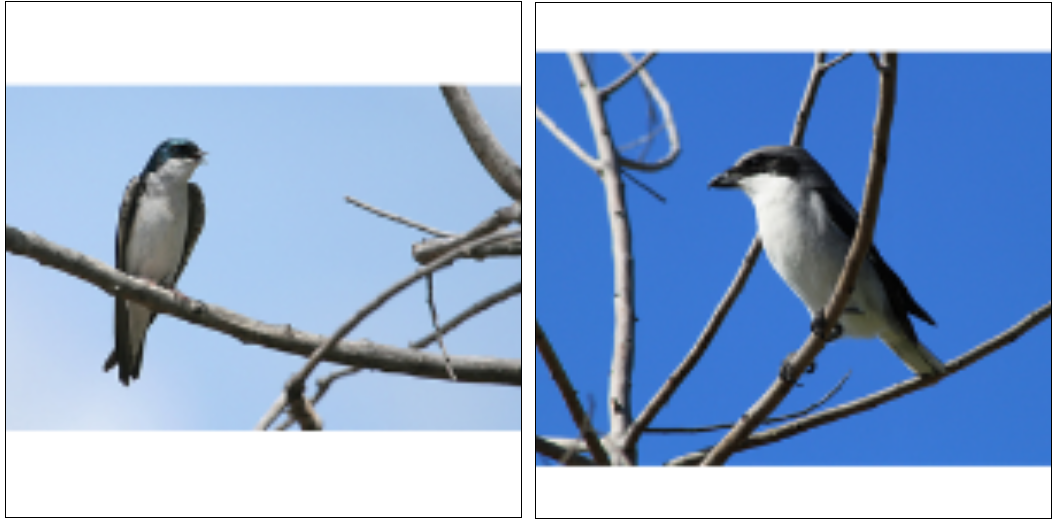
\includegraphics[ height=2cm, width=4cm]{\bilinearroot/figures/birds/birds_false_pos2.png}


% \\
% 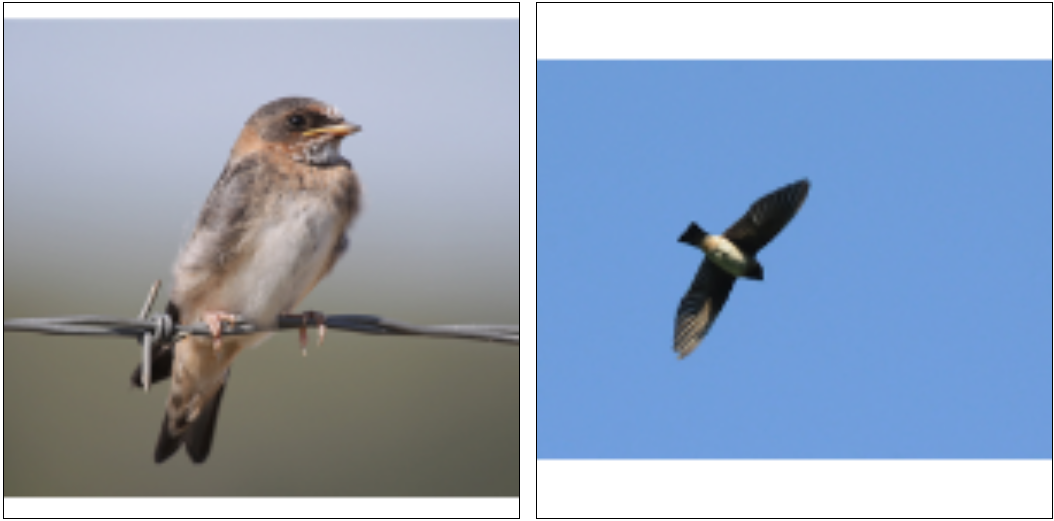
\includegraphics[ height=2cm, width=4cm]{\bilinearroot/figures/birds/birds_false_neg1.png}&
% 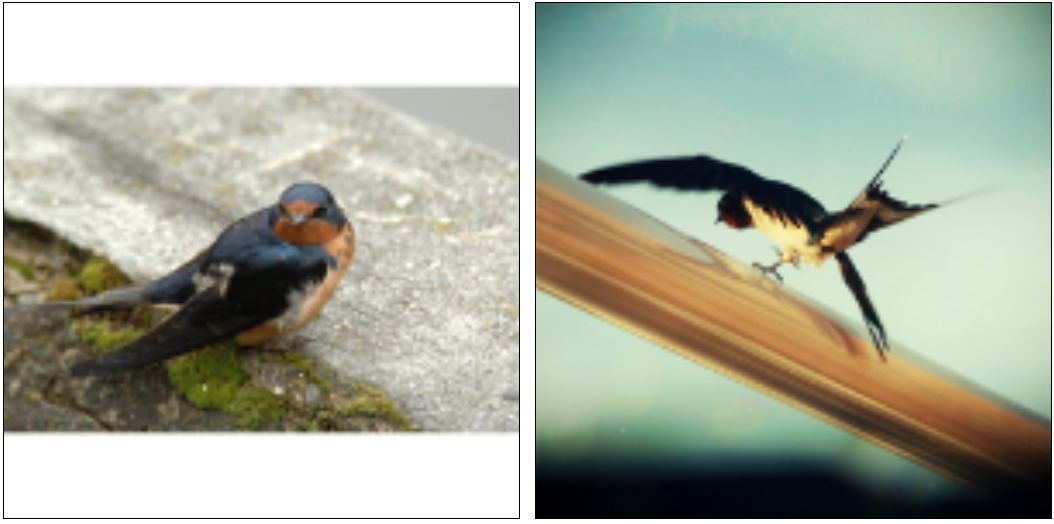
\includegraphics[ height=2cm, width=4cm]{\bilinearroot/figures/birds/birds_false_neg3.png}

% \end{tabular}
% \end{tabular} 
% \caption{Left-- difficult re-identification cases in the CUHK03 dataset \citep{li2014deepreid}. The pairs in the upper row show very similar images depicting different persons, the pairs in the lower row show dissimilar images depicting the same person. Right -- analogous cases for the CUB-Birds dataset for the fine-grained classification~\citep{Wah11}. There is a clear similarity between the challenges posed by the two tasks. Both re-identification and fine-grained classification deal with strong viewpoint variations, and often need to focus on small-scale fragments in order to distinguish subjects/classes. At the same time the re-identification task has a greater degree of alignment, and we therefore suggest a modification of the bilinear CNN exploiting the presenсe of such weak alignment in the re-identification case.}
% \label{fig:teaser}
% \end{figure*}


\begin{figure*}
\begin{center}
    

\begin{tabular}{c}
 
    
            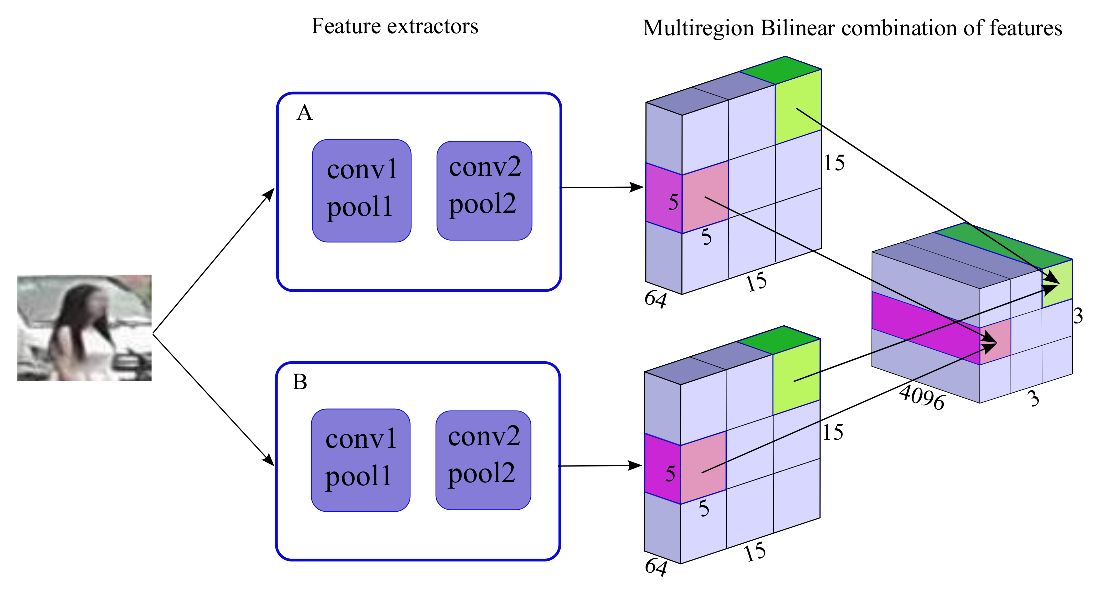
\includegraphics[width=0.7\textwidth]{\bilinearroot/figures/architecture/multiregion_bilinear.eps}\\
    (a)\\
            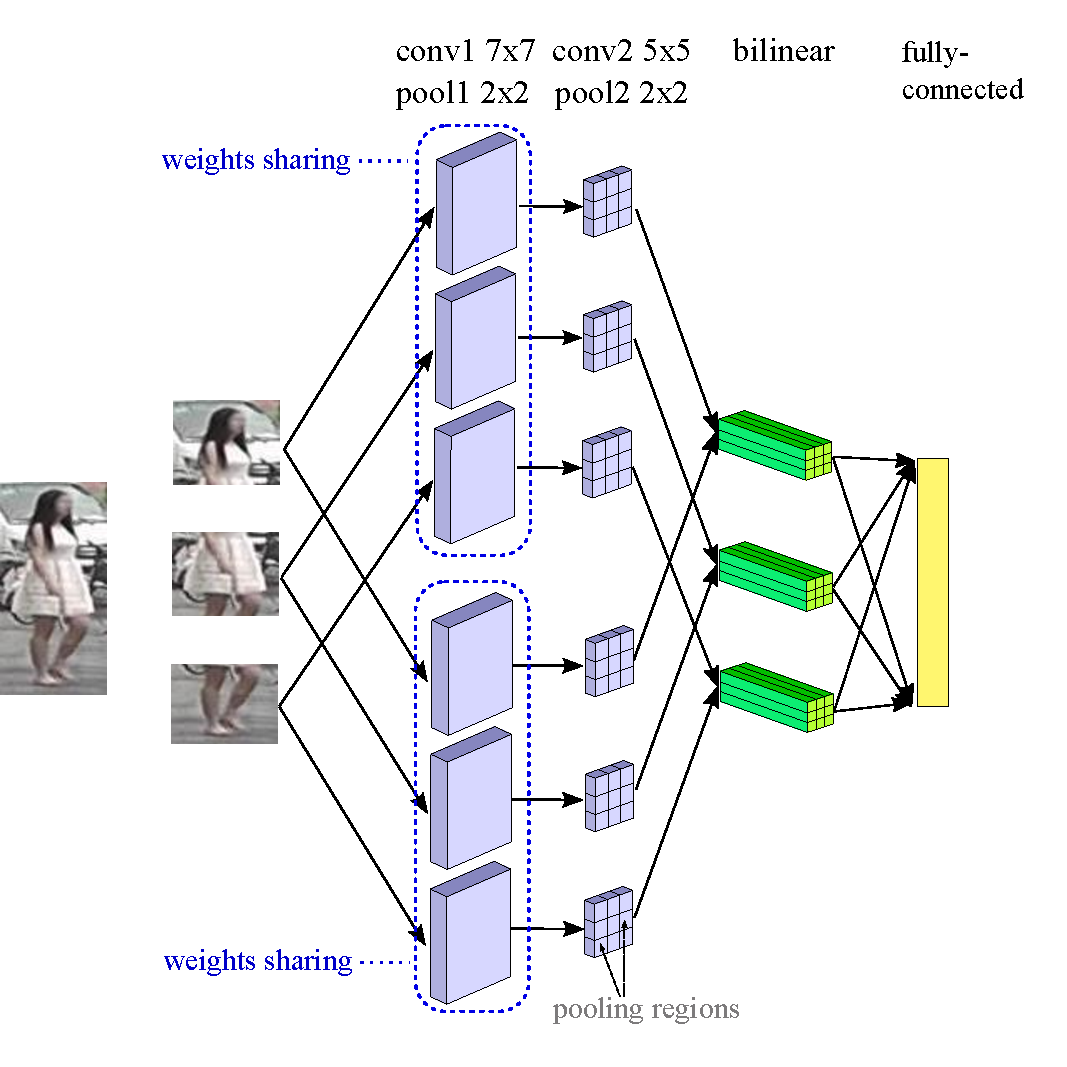
\includegraphics[width=0.7\textwidth]{\bilinearroot/figures/architecture/architecture.pdf}
            \\
    (b)\\
   
 \end{tabular}
        \caption{The proposed architecture for person re-identification: (a) - multi-region bilinear sub-network used for each of the three parts of the input image, (b) - the whole multi-region Bilinear CNN architecture that uses bilinear pooling over regions rather than the entire image. The new architecture achieves state-of-the-art performance over a range of benchmark datasets.}
        \label{fig:architecture}
    \end{center}
\end{figure*}

%\section{Related work}
\label{sect:related}

There are two main research directions dedicated to face recognition for low-quality data: (i) the face restoration approach and (ii) the domain adaptation approach. In the face restoration-based approach, low-quality images are enhanced and restored to facilitate recognition. The ability to reuse existing recognition systems that were developed for high-quality data comes as a natural benefit of such methods. Domain adaptation methods are conversely aimed to change the existing recognition systems so that they are better suited for the target domain (i.e.\ low resolution/quality images). We now provide a brief review of both approaches.

\subsection{Face restoration methods}

There is a vast range of methods that perform face restoration. In most of them, different degradation types are considered separately. Pan \textit{et al.} \cite{pan2014deblurring} propose an effective face deblurring method based on approximating blur kernel followed by non-blind deconvolution. The blur kernel  approximation is guided by the known non-blurred exemplar with the structure similar to the input image structure. 

In Zhang \textit{et al.}~\cite{ZhangYZNH11}, deblurring and recognition tasks are considered simultaneously. They use a sparse representation of the input image in terms of the gallery image set. The blur kernel and representation coefficients are estimated iteratively. Classification is finally performed based on the classes with the highest coefficients in the sparse representation.  


A number of recent methods \cite{TuzelTH16,ZhuLLT16,xu2017learning,huang2017wavelet} explore the task of restoration of extremely low-resolution images using deep neural networks. All these works utilize the paired (aligned) learning scheme, where the high-resolution ground truth is known for every low-resolution image in the training set. The low-resolution training data are simulated using synthetic degradation of the initial high-resolution images. In \cite{xu2017learning} and \cite{TuzelTH16}, a generative adversarial network~(GAN)~\cite{goodfellow2014generative} is used to force the restoration network to produce more natural images. In \cite{huang2017wavelet}, an additional structure-based loss that uses wavelet transform is suggested for the same goal. While the results of these methods are impressive, there is no direct way to use the paired learning approaches for the arbitrary combination of degradation factors that one may encounter when analyzing real images captured by surveillance cameras. 

\subsection{Domain adaptation methods}

Several recent works are dedicated to domain adaptation in the context of different recognition tasks \cite{Volpi_2018_CVPR,Hong_2018_CVPR,Deng_2018_CVPR,Bousmalis_2017_CVPR,Murez_2018_CVPR}. In \cite{Murez_2018_CVPR}, 
\cite{Bousmalis_2017_CVPR} and \cite{Deng_2018_CVPR}, image-level domain adaptation is performed for segmentation, classification and similarity learning (person re-identification) correspondingly. Hong \textit{et al.} \cite{Hong_2018_CVPR} and Volpi \textit{et al.} \cite{Volpi_2018_CVPR} resort to feature-level domain adaptation for segmentation and classfication tasks. Both feature-level and image-level techniques are used in \cite{Hoffman17}.

Some of the aforementioned methods \cite{Hoffman17,Deng_2018_CVPR,Murez_2018_CVPR} employ CycleGAN framework  to change the domain of training data for classification, segmentation, and person re-identification. Here we explore a similar approach for the task of face recognition in the presence of complex degradation factors.

Hong \textit{et al.} \cite{HongIRY17} and
Sohn \textit{et al.} \cite{SohnLZY0C17} approach face recognition tasks for low-quality image domain. They consider image degradation as a domain shift and perform feature-level unsupervised domain adaptation based on adversarial learning showing better recognition results. 
The works \cite{HongIRY17} and \cite{SohnLZY0C17} are very related to ours: the authors show that domain-specific data augmentation is essential for training face recognition systems. 
 However, in both works, the data augmentation is performed 'by hand' (the degradation types and hyper-parameters for transforms are chosen and fixed), while we augment the training data in an automatic manner utilizing the CycleGAN framework, which can also be viewed as an image-level domain adaptation.
%Additionally, in contrast to \cite{HongIRY17}, we do not consider extremely large pose variation. Instead, we are more focused on the image degradation factors (e.g. the combination of small size, blur, JPEG-compression). 
Differently from \cite{SohnLZY0C17}, where evaluation is performed for the Youtube faces dataset, we approach the task in the presence of the somewhat stronger domain shift, as our test data are captured by surveillance cameras and are mostly of much lower quality.




%Some works already successfully use CycleGAN technique to perform an unsupervised domain adaptation. \cite{CYCADA} approached semantic segmentation. % add avput CYCADA

%recognition and reconstruction approaches
% Several existing works consider restoration and recognition problems jointly. In some works, authors apply the recognition-based priors to achieve better restoration results. \cite{TODO , Xu} 

% There are also approaches jointly performing explicit recognition and restoration
% In \cite{TODO Close  the  loop:  Jointblind  image  restoration  and  recognition  with sparse representation prior , Baker} The  proposed  approaches  perform  recognition  using  a  limited  number  of  gallery  images.   In parallel, they reconstruct the input image and classify it based on labels of the most relevant examples found in the train set.

 
% One of the baselines used in this work applies the similar scheme: CycleGAN framework is used to transfer the low-quality test data into the high-quality domain, the domain classifier serves as 'restoration' loss. We additionally introduce the recognition component into this scheme: another baseline is the same CycleGAN but with domain classifier based that is learned using features calculated with the pre-trained face recognition network.




\section{Evaluated approaches}
\label{sect:method}
\bigskip
\indent\textbf{Face recognition for the low-quality image domain}\\
%\subsubsection{Face recognition for the low-quality image domain}
\label{sect:strategies}
In this work we consider and compare two main approaches to face recognition for surveillance data: 1) restoration-based approach and 2) domain adaptation of existing face recognition neural networks. 

We consider two facial image domains: \begin{itemize}
\item domain $T: \{X^{T}_{i} \}_{i=0}^{N_T}$ that includes low-quality facial images $X^{T}_{i}$ captured using surveillance cameras. Usually, there are no identity labels provided, as assigning identity labels is quite challenging and may not even be feasible.
\item domain $S: \{(X^{S}_{i}, Y^{S}_{i})\}_{i=0}^{N_S}$ that includes facial images $X^{S}_{i}$ harvested from the Internet. These images are usually of higher quality and are taken in good lighting conditions. We assume that the data in this domain are supplied with identity labels $Y_i$.
\end{itemize}  

According to the available labeling, we can consider two different pipelines for building face recognition systems for surveillance data. The first option is the restoration-based approach when we use transform $F^{T \rightarrow S}: T \longrightarrow S$ as a face restoration method and then apply existing recognition neural network $R^{S}$ that is pre-trained on images from the domain $S$. The second option is to use the transform $F^{S \rightarrow T}: S \longrightarrow T$ to transfer the large collections of labeled training data to the target domain of surveillance images. In this scenario, we retrain the existing face recognition networks resulting in the new adapted model $R^{T}$.

More formally, we consider the following two pipelines for face recognition in the domain $T$.  We denote $d^{T}$ and $d^{S}$ the descriptors produced by the domain-specific face recognition models $R^{T}$ and $R^{S}$. These descriptors may be used e.g.\ to identify matching and non-matching faces based on the distances between them. 
 
$F^{T \rightarrow S}: T \longrightarrow S$ and $F^{S \rightarrow T}: B \longrightarrow A$ are the image-level domain transfer mappings. In the restoration-based approach, we train the recognition model $R^{S}$ using labeled data  $\{(X^{S}_{i}, Y^{S}_{i})\}$ where $X^{S}_{i} \subseteq B$. We then test the learned model by computing the descriptors $d^{S}$ after applying the network $F^{T \rightarrow S}$:  $d^{S} = R^{S}(X^{T\rightarrow S}) = R^{S}(F^{T \rightarrow S}(X^{T}))$

In the domain adaptation approach, we train the recognition network $R^{T}$ using labeled data $\{(X^{S \rightarrow T}_{i}, Y^{S}_{i})\}$, where the training examples $X^{S \rightarrow T }_{i} = F^{S \rightarrow T}(X^{S}_i)$, $X^{S}_i \subseteq S$ are obtained by transforming the high-quality images to the low-quality domain using the learned transformation $F^{S \rightarrow T}$. In this case, we apply the learned network directly to the low-quality images by computing and working with their descriptors $d^{T} = R^{T}(X^{T})$. The two approaches are compared below.


%image describing train and test time for both schemes
\bigskip
\indent\textbf{Learning domain transfer mappings}\\
%\subsubsection{Learning domain transfer mappings}
\label{sect:domain_transfer}
We use the CycleGAN approach~\citep{ZhuPIE17} to simultaneously learn the domain transfer mappings in both directions: $ F^{T \rightarrow S}: T  \longrightarrow S$ (restoration-based approach) and  $F^{S \rightarrow T}: S \longrightarrow T$ (domain adaptation approach). Here we describe the objective functions used for learning the domain transfer architecture.

We use the variant of CycleGAN similar to the one introduced in \citep{LiuNIPS2017} as we found it resulting in more stable and visually more plausible results for our task than the original framework \citep{ZhuPIE17}. Following \citep{LiuNIPS2017}, we decompose the domain transfer mappings into the compositions of encoders and generators: $F^{T \rightarrow S} = G^{S} \odot E^{T} $ and $F^{S \rightarrow T} = G^{T} \odot E^{S} $. Here, the encoders $E^{T}$ and $E^{S}$ transfer input images to the latent space, and generators $G^{S}$ and $G^{T}$ map the input latent codes to the domains $S$ and $T$.
 
For inputs $X^{T} \subseteq T $ and $X^{S} \subseteq S $ the results of their transfer to the opposite domain will be:
\begin{equation}
    X^{T \rightarrow S} = F^{T \rightarrow S}(X^{T}; \theta^{T}_F) = G^{S}(E^{T}(X^{T}))  
\end{equation}
\begin{equation}
    X^{S \rightarrow T} = F^{S \rightarrow T}(X^{S}; \theta^{S}_F) = G^{T}(E^{S}(X^{S}))
\end{equation}

The objective function used by the CycleGAN approach for learning is composed of the two symmetric parts:
\begin{equation}
\mathcal{L} = \mathcal{L}^{T} + \mathcal{L}^{S},
\end{equation} where $\mathcal{L}^{T}$ further decomposes as:
\begin{equation}\label{eq:domain_loss}
     \mathcal{L}^{T} = \mathcal{L}_{\text{GAN}}^T + \lambda_1 \mathcal{L}_{\text{cycle}}^T + \lambda_2 \mathcal{L}_{\text{rec}}^T,
\end{equation}
while $\mathcal{L}^{S}$ has same structure as $\mathcal{L}^{T}$:
\begin{equation}\label{eq:domain_loss2}
     \mathcal{L}^{S} = \mathcal{L}_{\text{GAN}}^S + \lambda_1 \mathcal{L}_{\text{cycle}}^S + \lambda_2 \mathcal{L}_{\text{rec}}^S,
\end{equation}


We now describe each of the terms in \eq{domain_loss}.
The GAN loss serves as the optimization objective for the domain transfer: 

\begin{dmath}
\mathcal{L}_{\text{GAN}}^A = 
    \min_{\theta^{S}_F} \max_{\theta^{T}_D} \mathbb{E}_{x \sim p_{X^{T}}} \log D^{T}(x) +
    \mathbb{E}_{x \sim p_{X^{S}}} \log \big(1 - D^{T}(F^{S \rightarrow T}(x)) \big)\,
\end{dmath}


Here, $D^{T}(X;\theta^{T}_D)$ and $D^{S}(X;\theta^{S}_D)$ are discriminators for the domains $T$ and $S$ that are trained in parallel with the training of the domain transforms.

The other two terms are the so-called cycle consistency loss: 
\begin{equation}
\mathcal{L}_{\text{cycle}}^T = L_1(F^{S \rightarrow T}(F^{T \rightarrow S}(X^{T})), X^{T})  
\end{equation}
and the reconstruction loss:
\begin{equation}
\mathcal{L}_{\text{rec}}^T = L_1(G^{T}(E^{T}(X^{T})), X^{T}) 
\end{equation}
In both terms, $L_1(\cdot,\cdot)$ denotes the $L_1$ distance.

We show the results of transferring the Internet and surveillance images to the other domain in figure \ref{fig:lr_hr_gan_res_ytube_initial_degraded}. While these results look interesting, we do not analyze their visual quality, as we are ultimately interested in the recognition performance rather than obtained visually-convincing images.

\bigskip
\indent\textbf{Learning face recognition models}\\
%\subsubsection{Learning face recognition models}
\label{sect:face_recognition}
In both scenarios that we compare in this paper, we need to train a face recognition model that turns images into vectorial descriptors. This happens either in domain $S$ (in the face restoration approach) or in domain $T$ (in the domain adaptation approach).

In either case, the goal of the training is to build a deep convolutional network that converts face images to the descriptors, such that matching face images have close descriptors and non-matching face descriptors have dissimilar descriptors. We use the Binomial Deviance loss~\citep{Yi14} to perform such training \eq{bindev}. We note that the choice of a particular metric learning loss is orthogonal to our study.

Alternatively to the models trained using the setting discussed above, we also consider reusing the VGG face model trained by the authors of~\citep{parkhi2015deep} on the VGG-face dataset.
\section{Experiments}
\label{sec:4}
\subsection{ModelNet40 dataset}
In our experiments we used well known data set of 3D objects ModelNet40.
It is a subset of 40 classes of larger data set called ModelNet \cite{wu20153d} that contains different 3D CAD models in OFF format.

The total size of ModelNet40 data set $12311$.
The data set is split into training and test subsets, their sizes are $9843$ and $2468$ correspondingly.
The data set is not balanced.
Number of samples per class vary: from 64 to 889, see Figure \ref{fig:modelnet_classes}.

\begin{figure}
	\centering
    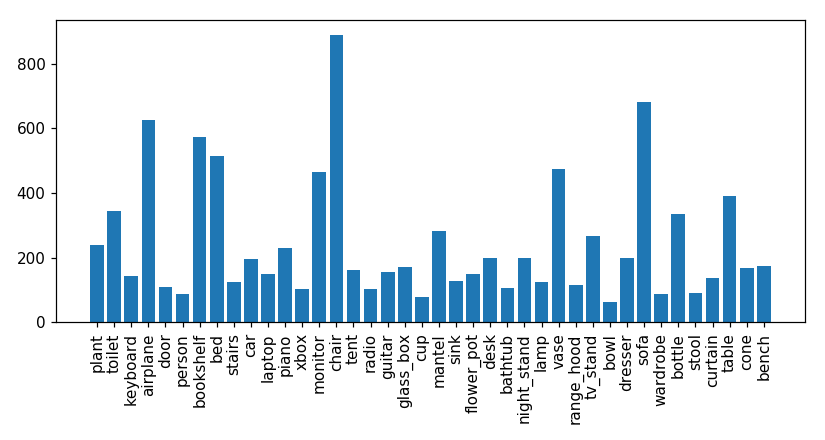
\includegraphics[width=\textwidth]{Figures/shape_retrieval/modelnet_classes.png}
    \caption{ModelNet40 data set: distribution of samples per class.}
    \label{fig:modelnet_classes}
\end{figure}

\subsection{Implementation details}
To demonstrate the impact that the triplet based training has on the performance of CNN descriptors
we use a deep network architecture shown in a Table~\ref{tab:net-architecture}. This network was implemented in PySparseConvNet, which is our modification of the SparseConvNet library \cite{graham2014spatially}. Besides new loss functions PySparseConvNet can be accessed from Python for a more interactive usage.

When forming a triplet for training we choose uniformly randomly a positive pair of objects from one class
and select a negative sample uniformly randomly from one of other classes.

For the optimization we use the SGD \cite{bottou-tricks-2012}, and the training is done
\begin{itemize}
\item in batches of size from $45$ to $90$ depending on a GPU video memory,
\item with a learning rate of $0.002$,
\item and a momentum equal to $0.99$.
\end{itemize}
Training can take up to a week on a server with advanced GPU, such as NVIDIA Titan X or GTX980ti.

\begin{figure}
\centering
\begin{tabular}{ccccc}
  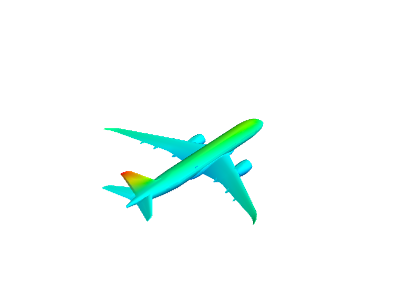
\includegraphics[width=0.19\columnwidth]{Figures/shape_retrieval/pic_airplane_solid.png} &
  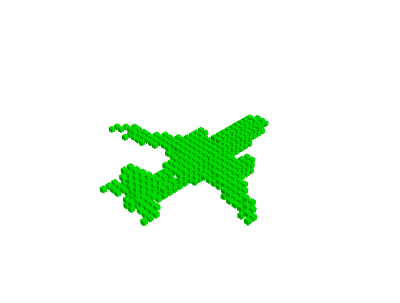
\includegraphics[width=0.19\columnwidth]{Figures/shape_retrieval/pic_airplane_30_solid.png} &
  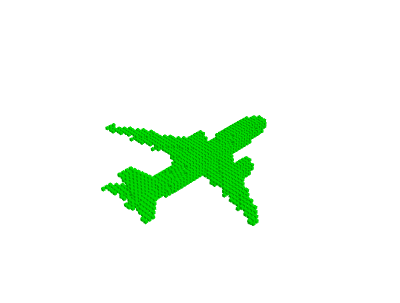
\includegraphics[width=0.19\columnwidth]{Figures/shape_retrieval/pic_airplane_50_solid.png} &
  \includegraphics[width=0.19\columnwidth]{Figures/shape_retrieval/pic_airplane_70_solid.png} &
  \includegraphics[width=0.19\columnwidth]{Figures/shape_retrieval/pic_airplane_100_solid.png} \\
% (a) first & (b) second \\
 \includegraphics[width=0.19\columnwidth]{Figures/shape_retrieval/pic_person_solid.png} &
 \includegraphics[width=0.19\columnwidth]{Figures/shape_retrieval/pic_person_30_solid.png} &
 \includegraphics[width=0.19\columnwidth]{Figures/shape_retrieval/pic_person_50_solid.png} &
 \includegraphics[width=0.19\columnwidth]{Figures/shape_retrieval/pic_person_70_solid.png} &
 \includegraphics[width=0.19\columnwidth]{Figures/shape_retrieval/pic_person_100_solid.png} \\

 \includegraphics[width=0.19\columnwidth]{Figures/shape_retrieval/pic_car_solid.png} &
 \includegraphics[width=0.19\columnwidth]{Figures/shape_retrieval/pic_car_30_solid.png} &
 \includegraphics[width=0.19\columnwidth]{Figures/shape_retrieval/pic_car_50_solid.png} &
 \includegraphics[width=0.19\columnwidth]{Figures/shape_retrieval/pic_car_70_solid.png} &
 \includegraphics[width=0.19\columnwidth]{Figures/shape_retrieval/pic_car_100_solid.png} \\
\end{tabular}
\caption{Examples of some objects voxelizations at different resolutions $30$, $50$, $70$, $100$ (from left to right), left-most objects are depicted using original meshes}
\label{fig:voxels-examples}
\end{figure}


We train Sparse 3D Convolutional Neural Network (S3DCNN) on the 3D shape classification dataset by splitting it into  training and validation subsets, adding augmentation of data to achieve rotational and translational invariance. After training a model on a dataset of pairs, we use it to embed voxel representations of 3D meshes into $192$-dimensional space. The retrieval consist of ranking search objects by a cosine distance of vectors from a query vector.

The most popular metrics for evaluating retrieval performance are
\begin{itemize}
\item Precision-Recall Curve shows a trade-off between these two measures and how quickly the precision drops with the recall increase,
\item Mean average precision (mAP). Given a query, its average precision is the average of all precision values computed on all relevant objects in the retrieved list. Given several queries, the mean average precision (mAP) is the mean of average precisions for these queries. 
\end{itemize}
We evaluated mAP for different voxel rendering sizes of 3D shapes both at train and test times, see also Figure~\ref{fig:voxels-examples}.

To check if our model is comparable with other architectures, we consider a classification task. So, we trained our model for the classification task using the ModelNet40 train subset with 
\begin{itemize}
\item SoftMax last layer for $200$ epochs,
\item with exponentially discounting learning rate,
\item and performed retrieval evaluation on the test subset,
\item taking $20$ images from every class, and ranking them w.r.t their $L2$-norm by activations taken from the $17$-th layer.
\end{itemize}

Results of these experiments are provided in Table~\ref{tab:classification}. We can see that in case of classification task setup our model is comparable in terms of the classification accuracy, but mAP values are worse. But in case of metric learning performace of S3DCNN on mAP metric is much better.
Superior performance of retrieval task with MVCNN is not a surprising result, since MVCNN uses neural nets, pre-trained on ImageNet. On the other hand our model only requires 3D Shape dataset to learn.

In Figure~\ref{fig:map_for_rs} we provide the dependence of mAP on the input spatial resolution. We can see that the retrieval performance improves with increase in the input spatial resolution up to around $45-50$, after that it drops slightly and goes to plateau. It can be attributed to the insufficient amount of layers for the same scale of features, that can be separated in higher layers. Light blue color shows range of mAP on validation for top $30$ trained architectures.


\begin{figure}[!tbp]
\vspace{-20pt}
\centering
\begin{minipage}[b]{0.45\textwidth}
  \centering
  \includegraphics[width=\columnwidth]{Figures/shape_retrieval/new_map_to_rs.pdf}
  \caption{Dependence of the retrieval performance on the input spatial resolution}
  \label{fig:map_for_rs}
\end{minipage}
\begin{minipage}[b]{0.45\textwidth}
  \centering
  \includegraphics[width=\columnwidth]{Figures/shape_retrieval/pr_curves_comp}
  \caption{Precision-Recall curve for our method}
  \label{fig:pr_curve}
\end{minipage}
\end{figure}


We would like to note that in Figure~\ref{fig:map_for_rs} mAP values provided for different validation epochs and variability of best model can be explained by difference in total learning time.

% \begin{itemize}
% \item In Table~\ref{tab:classification} for the retrieval we used features from the last but one layer of the network,
% \item In Figure~\ref{fig:map_for_rs} we used learning with the triplet loss, for which we still have to better adjust the architecture and learning rate schedule.
% \end{itemize}


\begin{figure}
\includegraphics[height=0.76\textheight]{\bilinearroot/figures/market_random.png}
\caption{The result of the proposed architecture on the Market-1501 dataset for a random subset of queries. The queries are shown on the left, and the remaining images in each row show the closest matches in the gallery dataset.}
\label{fig:market_retrieval}
\end{figure}


\section{Conclusion}
\label{sect:conclusion}

% Discuss your conclusions in order of most to least important.

In this chapter, we have compared the image-based domain adaptation techniques for face recognition in the presence of strong image degradation. We consider the recently proposed CycleGAN approach for learning mappings between the two domains of surveillance data and Internet face images. We demonstrate that the strategy of transferring the labeled Internet data to the surveillance domain and subsequent retraining the face recognition network helps to improve the recognition quality on real surveillance test data. We have investigated the variants of this approach, and have demonstrated that training on both transferred and original Internet data leads to the optimal performance. Finally, we show that in the case of our domain pair, the image-level adaptation approach outperforms feature-level domain adaptation. 

%Compare your results with those from other studies: Are they consistent? If not, discuss possible reasons for the difference.
We found our results consistent with \cite{SohnLZY0C17}, where face recognition for the low-quality is also considered. In \cite{SohnLZY0C17},  verification accuracy was improved using carefully chosen data augmentation. It is an interesting fact, that the improvement remained noticeable even when the data augmentation and the feature-level domain adaptation were applied simultaneously. Here, in contrast, we suggest performing the data augmentation in a more automatic way. Although we do not experiment with the combination of feature-level and image-level approaches to domain adaptation, we compare them independently. The combination of these adaptation techniques may further improve the results.


% Mention any inconclusive results and explain them as best you can. You may suggest additional experiments needed to clarify your results.
In our experiments, best results were achieved with training on both domains. An explanation can be given that the domain transfer model is imperfect and may push different images of the same identity too far as we do not use any kind of verification loss for training (ideally, this would require another pre-trained network for the low-quality domain, which essentially is the goal of this work). Therefore, keeping the initial data in the training set may result in less overfitting. %This can be explained by the fact that our target domain is not uniform in terms of data quality. We use two parts of the same track to generate matching pairs for each identity: e.g. these parts of each track differ in resolution (see \ref{fig:lr_hr_gan_res_ytube_initial_degraded}, columns $1$ and $3$). Therefore, using training data of diverse quality may lead to better results.  -- not true, checked.

% Briefly describe the limitations of your study to show reviewers and readers that you have considered your experiment’s weaknesses. Many researchers are hesitant to do this as they feel it highlights the weaknesses in their research to the editor and reviewer. However doing this actually makes a positive impression of your paper as it makes it clear that you have an in depth understanding of your topic and can think objectively of your research.

As an important negative result, we show that using CycleGAN-based restoration of lower-quality domain images by transferring them to the higher-quality domain does not bring consistent improvement to the recognition performance. We speculate that such transfer may distort some details of the images in a non-identity preserving way.

Our study considers a practically important domain of image data. 
We note, however, that our findings might not transfer to other pairs of domains in image adaptation.


% Discuss what your results may mean for researchers in the same field as you, researchers in other fields, and the general public. How could your findings be applied?
 
% State how your results extend the findings of previous studies.
% If your findings are preliminary, suggest future studies that need to be carried out.
% At the end of your Discussion and Conclusions sections, state your main conclusions once again.



% \newpage 
% \chapter{Domain-adversarial adaptation by backpropagation}
\label{chapt:gradrev}
%\section{Deep Domain Adaptation}

\def\x{{\mathbf x}}
\def\f{{\mathbf f}}

\def\S{{\cal S}}
\def\T{{\cal T}}

\def\R{{\mathds R}}

\def\tf{{\theta_f}}
\def\td{{\theta_d}}
\def\ty{{\theta_y}}
\def\htf{{\hat\theta_f}}
\def\htd{{\hat\theta_d}}
\def\hty{{\hat\theta_y}}

\subsection{The model}

We now detail the proposed model for the domain adaptation. We assume that the model works with input samples $\x \in X$, where $X$ is some input space and certain labels (output) $y$ from the label space $Y$. Below, we assume classification problems where $Y$ is a finite set ($Y=\{1,2,\dots L\}$), however our approach is generic and can handle any output label space that other deep feed-forward models can handle. We further assume that there exist two distributions $\S(x,y)$ and $\T(x,y)$ on $X\otimes Y$, which will be referred to as the source distribution and the target distribution (or the source domain and the target domain). Both distributions are assumed complex and unknown, and furthermore similar but different (in other words, $\S$ is ``shifted'' from $\T$ by some {\em domain shift}). 

Our ultimate goal is to be able to predict labels $y$ given the input $\x$ for the target distribution. At training time, we have an access to a large set of training samples $\{\x_1,\x_2,\dots,\x_N\}$ from both the source and the target domains distributed according to the marginal distributions $\S(\x)$ and $\T(\x)$. We denote with $d_i$ the binary variable ({\em domain label}) for the $i$-th example, which indicates whether $x_i$ come from the source distribution ($\x_i{\sim}\S(\x)$ if $d_i{=}0$) or from the target distribution ($\x_i{\sim}\T(\x)$ if $d_i{=}1$). For the examples from the source distribution ($d_i{=}0$) the corresponding labels $y_i \in Y$ are known at training time. For the examples from the target domains, we do not know the labels at training time, and we want to predict such labels at test time.

We now define a deep feed-forward architecture that for each input $\x$ predicts its label $y \in Y$ {\em and} its domain label $d \in \{0,1\}$. We decompose such mapping into three parts. We assume that the input $\x$ is first mapped by a mapping $G_f$ (a {\em feature extractor}) to a $D$-dimensional feature vector $\f \in \R^D$. The feature mapping may also include several feed-forward layers and we denote the vector of parameters of all layers in this mapping as $\tf$, i.e.\ $\f = G_f(\x;\tf)$. Then, the feature vector $\f$ is mapped by a mapping $G_y$ ({\em label predictor}) to the label $y$, and we denote the parameters of this mapping with $\ty$. Finally, the same feature vector $\f$ is mapped to the domain label $d$ by a mapping $G_d$ ({\em domain classifier}) with the parameters $\td$ (\fig{arch}).

During the learning stage, we aim to minimize the label prediction loss on the annotated part (i.e.\ the source part) of the training set, and the parameters of both the feature extractor and the label predictor are thus optimized in order to minimize the empirical loss for the source domain samples. This ensures the discriminativeness of the features $\f$ and the overall good prediction performance of the combination of the feature extractor and the label predictor on the source domain.

At the same time, we want to make the features $\f$ domain-invariant. That is, we want to make the distributions $S(\f) = \{G_f(\x; \tf)\,|\, \x{\sim}S(\x)\}$ and $T(\f) = \{G_f(\x; \tf)\,|\, \x{\sim}T(\x)\}$ to be similar. Under the {\em covariate shift} assumption, this would make the label prediction accuracy on the target domain to be the same as on the source domain~\cite{Shimodaira00}. Measuring the dissimilarity of the distributions $S(\f)$ and $T(\f)$ is however non-trivial, given that $\f$ is high-dimensional, and that the distributions themselves are constantly changing as learning progresses. One way to estimate the dissimilarity is to look at the loss of the domain classifier $G_d$, provided that the parameters $\td$ of the domain classifier have been trained to discriminate between the two feature distributions in an optimal way. 

This observation leads to our idea. At training time, in order to obtain domain-invariant features, we seek the parameters $\tf$ of the feature mapping that {\em maximize} the loss of the domain classifier (by making the two feature distributions as similar as possible), while simultaneously seeking the parameters $\td$ of the domain classifier that {\em minimize} the loss of the domain classifier. In addition, we seek to minimize the loss of the label predictor. 

More formally, we consider the functional:
\begin{gather} 
E(\tf,\ty,\td) =  \sum_{\substack{i=1..N\\d_i = 0}} L_y\left( \strut G_y(G_f(\x_i;\tf);\ty), y_i\right) -\nonumber\\ \lambda \sum_{i=1..N} L_d \left( \strut G_d(G_f(\x_i;\tf);\td), y_i\right) = \nonumber\\= \sum_{\substack{i=1..N\\d_i = 0}} L^i_y( \tf, \ty) - \lambda \sum_{i=1..N} L^i_d( \tf, \td) 
\label{eq:func}
\end{gather}
Here, $L_y(\cdot,\cdot)$ is the loss for label prediction (e.g.\ multinomial), $L_d(\cdot,\cdot)$ is the loss for the domain classification (e.g.\ logistic), while $L^i_y$ and $L^i_d$ denote the corresponding loss functions evaluated at the $i$-th training example. 

Based on our idea, we are seeking the parameters $\htf,\hty,\htd$ that deliver a saddle point of the functional \eq{func}:

\begin{gather}
(\htf,\hty) = \arg\min_{\tf,\ty} E(\tf,\ty,\htd)\,\label{eq:opt1}\\\label{eq:opt2}
\htd = \arg\max_\td E(\htf,\hty, \td)\,.
\end{gather}

At the saddle point, the parameters $\td$ of the domain classifier $\td$ minimize the domain classification loss (since it enters into \eq{func} with the minus sign) while the parameters $\ty$ of the label predictor minimize the label prediction loss. The feature mapping parameters $\tf$ {\em minimize} the label prediction loss (i.e.\ the features are discriminative), while {\em maximizing} the domain classification loss (i.e.\ the features are domain-invariant). The parameter $\lambda$ controls the trade-off between the two objectives that shape the features during learning.

Below, we demonstrate that standard stochastic gradient solvers (SGD) can be adapted for the search of the saddle point \eq{opt1}-\eq{opt2}.

\subsection{Optimization with backpropagation}

A saddle point \eq{opt1}-\eq{opt2} can be found as a stationary point of the following stochastic updates:

\begin{align}
\tf \quad &\longleftarrow \quad \tf \;-\; \mu \left(\frac{\partial L^i_y}{\partial \tf}-\lambda\frac{\partial L^i_d}{\partial \tf} \right) \label{eq:upd1}\\
\ty \quad &\longleftarrow \qquad \ty \;-\; \mu \frac{\partial L^i_y}{\partial \ty}\label{eq:upd2}\\
\td \quad &\longleftarrow \qquad \td \;-\; \mu \frac{\partial L^i_d}{\partial \td} \label{eq:upd3}
\end{align}
where $\mu$ is the learning rate (which can vary over time).

The updates \eq{upd1}-\eq{upd3} are very similar to stochastic gradient descent (SGD) updates for a feed-forward deep model that comprises feature extractor fed into the label predictor and into the domain classifier. The difference is the $-\lambda$ factor in \eq{upd1} (the difference is important, as without such factor, stochastic gradient descent would try to make features dissimilar across domains in order to minimize the domain classification loss). Although direct implementation of \eq{upd1}-\eq{upd3} as SGD is not possible, it is highly desirable to reduce the updates \eq{upd1}-\eq{upd3} to some form of SGD, since SGD (and its variants) is the main learning algorithm implemented in most packages for deep learning. 

Fortunately, such reduction can be accomplished by introducing a special {\bf gradient reversal layer} (GRL) defined as follows. The gradient reversal layer has no parameters associated with it (apart from the meta-parameter $\lambda$, which is not updated by backpropagation). During the forward propagation, GRL acts as an identity transform. During the backpropagation though, GRL takes the gradient from the subsequent level, multiplies it by $-\lambda$ and passes it to the preceding layer. Implementing such layer using existing object-oriented packages for deep learning is simple, as defining procedures for forwardprop (identity transform), backprop (multiplying by a constant), and parameter update (nothing) is trivial. 

The GRL as defined above is inserted between the feature extractor and the domain classifier, resulting in the architecture depicted in \fig{arch}. As the backpropagation process passes through the GRL, the partial derivatives of the loss that is downstream the GRL (i.e.\ $L_d$) w.r.t.\ the layer parameters that are upstream the GRL (i.e.\ $\tf$) get multiplied by $-\lambda$, i.e.\ $\frac{\partial L_d}{\partial \tf}$ is effectively replaced with $-\lambda\frac{\partial L_d}{\partial \tf}$. Therefore, running SGD in the resulting model implements the updates \eq{upd1}-\eq{upd3} and converges to a saddle point of \eq{func}.

Mathematically, we can formally treat the gradient reversal layer as a ``pseudo-function'' $R_\lambda(\x)$ defined by two (incompatible) equations describing its forward- and backpropagation behaviour:
\begin{align}
R_\lambda(\x) = \x\\
\frac{dR_\lambda}{d\x} = -\lambda \mathbf{I}
\end{align}
where $\mathbf{I}$ is an identity matrix.
We can then define the objective ``pseudo-function'' of $(\tf,\ty,\td)$ that is being optimized by the stochastic gradient descent within our method:
\begin{gather}
\tilde E(\tf,\ty,\td) =  \sum_{\substack{i=1..N\\d_i = 0}} L_y\left( \strut G_y(G_f(\x_i;\tf);\ty), y_i\right) +\nonumber\\ \sum_{i=1..N} L_d \left( \strut G_d(R_\lambda(G_f(\x_i;\tf));\td), y_i\right) \label{eq:pseudoobj}
\end{gather}

Running updates \eq{upd1}-\eq{upd3} can then be implemented as doing SGD for \eq{pseudoobj} and leads to the emergence of features that are domain-invariant and discriminative at the same time. After the learning, the label predictor $y(\x) = G_y(G_f(\x;\tf);\ty)$ can be used to predict labels for samples from the target domain (as well as from the source domain).

The simple learning procedure outlined above can be re-derived/generalized along the lines suggested in \cite{Goodfellow14} (see \cite{SuppMat}).

% \subsection{Relation to $ \mathcal{H} \Delta \mathcal{H} $-distance}
% \label{sect:theory}

% In this section we give a brief analysis of our method in terms of $ \mathcal{H} \Delta \mathcal{H} $-distance \cite{Ben10,Cortes11} which is widely used in the theory of non-conservative domain adaptation. Formally,
% \begin{multline}
%   d_{\mathcal{H} \Delta \mathcal{H}} (\mathcal{S}, \mathcal{T}) = 2 \sup_{h_1, h_2 \in \mathcal{H}} \left| P_{\mathbf{f} \sim \mathcal{S}} [h_1(\mathbf{f}) \neq h_2(\mathbf{f})] - \right. \\
%   \left. - P_{\mathbf{f} \sim \mathcal{T}} [h_1(\mathbf{f}) \neq h_2(\mathbf{f})] \right|
% \label{eq:hdh_dist}
% \end{multline}
% defines a discrepancy distance between two distributions $ \mathcal{S} $ and $ \mathcal{T} $ w.r.t. a hypothesis set $ \mathcal{H} $. Using this notion one can obtain a probabilistic bound \cite{Ben10} on the performance $ \varepsilon_\mathcal{T}(h) $ of some classifier $ h $ from $ \mathcal{T} $ evaluated on the target domain given its performance $ \varepsilon_\mathcal{S}(h) $ on the source domain:
% \begin{equation}
%   \varepsilon_\mathcal{T}(h) \leq \varepsilon_\mathcal{S}(h) + \frac{1}{2} d_{\mathcal{H} \Delta \mathcal{H}} (\mathcal{S}, \mathcal{T}) + C \, ,
% \end{equation}
% where $ \mathcal{S} $ and $ \mathcal{T} $ are source and target distributions respectively, and $ C $ does not depend on particular $ h $. 

% Consider fixed $ \mathcal{S} $ and $ \mathcal{T} $ over the representation space produced by the feature extractor $ G_f $ and a family of label predictors $ \mathcal{H}_p $. We assume that the family of domain classifiers $ \mathcal{H}_d $ is rich enough to contain the symmetric difference hypothesis set of $ \mathcal{H}_p $:
% \begin{equation}
%   \mathcal{H}_p \Delta \mathcal{H}_p = \left\{ h \, | \, h = h_1 \oplus h_2 \, , \; h_1, h_2 \in \mathcal {H}_p \right\} \, .
% \end{equation}
% It is not an unrealistic assumption as we have a freedom to pick $ \mathcal{H}_d $ whichever we want. For example, we can set the architecture of the domain discriminator to be the layer-by-layer concatenation of two replicas of the label predictor followed by a two layer non-linear perceptron aimed to learn the \texttt{XOR}-function. Given the assumption holds, one can easily show that training the $ G_d $ is closely related to the estimation of $ d_{\mathcal{H}_p \Delta \mathcal{H}_p} (\mathcal{S}, \mathcal{T}) $. Indeed, 
% \begin{equation}
% \begin{split}
%   &d_{\mathcal{H}_p \Delta \mathcal{H}_p}  (\mathcal{S}, \mathcal{T}) =\\ 
%   & = 2 \sup_{h \in \mathcal{H}_p \Delta \mathcal{H}_p} \left| P_{\mathbf{f} \sim \mathcal{S}} [h(\mathbf{f}) = 1] - P_{\mathbf{f} \sim \mathcal{T}} [h(\mathbf{f}) = 1] \right| \leq \\
%   & \leq 2 \sup_{h \in \mathcal{H}_d} \left| P_{\mathbf{f} \sim \mathcal{S}} [h(\mathbf{f}) = 1] - P_{\mathbf{f} \sim \mathcal{T}} [h(\mathbf{f}) = 1] \right| = \\
%   & = 2 \sup_{h \in \mathcal{H}_d} \left| 1 - \alpha(h) \right| = 2 \sup_{h \in \mathcal{H}_d} \left[ \alpha(h) - 1 \right]
% \end{split}
% \end{equation}
% where $ \alpha(h) = P_{\mathbf{f} \sim \mathcal{S}} [h(\mathbf{f}) = 0] + P_{\mathbf{f} \sim \mathcal{T}} [h(\mathbf{f}) = 1] $ is maximized by the optimal $ G_d $.

% Thus, optimal discriminator gives the upper bound for $ d_{\mathcal{H}_p \Delta \mathcal{H}_p}  (\mathcal{S}, \mathcal{T}) $. At the same time, backpropagation of the reversed gradient changes the representation space so that $ \alpha(G_d) $ becomes smaller effectively reducing $ d_{\mathcal{H}_p \Delta \mathcal{H}_p}  (\mathcal{S}, \mathcal{T}) $ and leading to the better approximation of $ \varepsilon_\mathcal{T}(G_y) $ by $ \varepsilon_\mathcal{S}(G_y) $.

%
\subsection{Experiments with Deep Image Descriptors for Re-Identification}

% In this section we discuss the application of the described adaptation method to person re-identification \textit{(re-id}) problem.  The task of person re-identification is to associate people seen from different camera views. More formally, it can be defined as follows: given two sets of images from different cameras (\textit{probe} and \textit{gallery}) such that each person depicted in the probe set has an image in the gallery set,  for each image of a person from the probe set find an image of the same person in the gallery set.  Disjoint camera views, different illumination conditions, various poses and low quality of data make this problem difficult  even for humans (\eg, \citet{LiuLGW13} reports human performance at Rank1=$71.08\%$).  

% Unlike classification problems that are discussed above, re-identification problem implies that each image is mapped to a vector descriptor. The distance between descriptors is then used to match images from the probe set and the gallery set.
% To evaluate results of re-id methods the \textit{Cumulative Match Characteristic} (CMC) curve is commonly used. It is a plot of the identification rate (recall) at rank-$k$, that is the probability of the matching gallery image to be within the closest $k$ images (in terms of descriptor distance) to the probe image.

% Most existing works train descriptor mappings and evaluate them within the same data set containing images from a certain camera network with similar imaging conditions. Several papers, however, observed that the performance of the resulting re-identification systems drops very considerably when descriptors trained on one data set and tested on another. It is therefore natural to handle such cross-domain evaluation as a domain-adaptation problem, where each camera network (data set) constitutes a domain.

% Recently, several papers  with significantly improved re-identification performance \citep{ZhangS14a,ZhaoOW14,Paisitkriangkrai15} have been presented, with \citet{MaLYL15} reporting good results in cross-data-set evaluation scenario. At the moment, deep learning methods \citep{YiLL14} do not achieve state-of-the-art results probably because of the limited size of the training sets. Domain adaptation thus represents a viable direction for improving deep re-identification descriptors.

% \subsubsection{Data Sets and Protocols} 

% Following \citet{MaLYL15}, we use PRID \citep{Hirzer_h.:person}, VIPeR \citep{Gray07evaluatingappearance}, CUHK \citep{LiW13} as target data sets for our experiments.  

%------------------------to main intro------------
%The \textit{PRID} data set exists in two versions, and as in \citep{MaLYL15} we use a single-shot variant. It contains images of $385$ persons viewed from camera A and images of $749$ persons viewed from camera B,  $200$ persons appear in both cameras. The \textit{VIPeR} data set also contains images taken with two cameras, and in total $632$ persons are captured, for every person there is one image for each of the two camera views. The \textit{CUHK} data set consists of images from five pairs of cameras, two images for each person from each of the two cameras. We refer to the subset of this data set that includes the first pair of cameras only as \textit{CUHK/p1} (as most papers use this subset).

% We perform extensive experiments for various pairs of data sets, where one data set serves as a source domain, \ie, it is used to train a descriptor mapping in a supervised way with known correspondences between probe and gallery images. The second data set is used as a target domain, so that images from that data set are used without probe-gallery correspondence.

% In more detail, CUHK/p1 is used for experiments when CUHK serves as a target domain and two settings (``whole CUHK'' and CUHK/p1) are used for experiments when CUHK serves as a source domain. Given PRID as a target data set, we randomly choose 100 persons appearing in both camera views as training set. The images of the other 100 persons from camera A are used as probe, all images from camera B excluding those used in training (649 in total) are used as gallery at test time. For VIPeR, we use random 316 persons for training and all others for testing. For CUHK, 971 persons are split into 485 for training and 486 for testing.
% Unlike \citet{MaLYL15}, we use all images in the first  pair of cameras of CUHK instead of choosing one image of a person from each camera view. We also performed two experiments with all images of the whole CUHK data set as source domain and VIPeR and PRID data sets as target domains as in the  original paper \citep{YiLL14}.
------------------
\newlength\reidheight
\setlength{\reidheight}{2.5cm}

\addtolength{\tabcolsep}{-3pt}

\begin{figure*}
\centering
\begin{tabular}{cccc|cccc|cccc}
\includegraphics[height=\reidheight]{Chapters/gradrev/figures/dataset_samples/viper/a/000_45.png}&
\includegraphics[height=\reidheight]{Chapters/gradrev/figures/dataset_samples/viper/b/000_45.png}&
\includegraphics[height=\reidheight]{Chapters/gradrev/figures/dataset_samples/viper/a/001_45.png}&
\includegraphics[height=\reidheight]{Chapters/gradrev/figures/dataset_samples/viper/b/002_90.png}&
\includegraphics[height=\reidheight]{Chapters/gradrev/figures/dataset_samples/PRID/a/img_0001.png}&
\includegraphics[height=\reidheight]{Chapters/gradrev/figures/dataset_samples/PRID/b/img_0001.png}&
\includegraphics[height=\reidheight]{Chapters/gradrev/figures/dataset_samples/PRID/a/img_0002.png}&
\includegraphics[height=\reidheight]{Chapters/gradrev/figures/dataset_samples/PRID/b/img_0003.png}&
\includegraphics[height=\reidheight]{Chapters/gradrev/figures/dataset_samples/cuhk/a/001_00005.png}&
\includegraphics[height=\reidheight]{Chapters/gradrev/figures/dataset_samples/cuhk/b/001_00221.png}&
\includegraphics[height=\reidheight]{Chapters/gradrev/figures/dataset_samples/cuhk/a/002_00280.png}&
\includegraphics[height=\reidheight]{Chapters/gradrev/figures/dataset_samples/cuhk/b/003_00403.png}\\
\multicolumn{4}{c}{VIPER}&
\multicolumn{4}{c}{PRID}&
\multicolumn{4}{c}{CUHK}
\end{tabular}
\caption{Matching and non-matching pairs of probe-gallery images from different person re-identification data sets. The three data sets are treated as different domains in our experiments.}
\label{fig:reidsamples}
\end{figure*}

\addtolength{\tabcolsep}{3pt}

Following \citet{YiLL14}, we augmented our data with mirror images, and during test time we calculate similarity score between two images as the mean of the four scores corresponding to different flips of the two compared images. In case of CUHK, where there are 4 images (including mirror images) for each of the two camera views for each person, all 16 combinations' scores are averaged. 

\subsubsection{CNN architectures and Training Procedure} 

In our experiments, we use siamese architecture described in \citet{YiLL14} (\textit{Deep Metric Learning} or \textit{DML}) for learning deep image descriptors on the source data set.
This architecture incorporates two convolution layers (with $7\times7$ and $5\times5$ filter banks), followed by ReLU and max pooling, and one fully-connected layer, which gives $500$-dimensional descriptors as an output. There are three parallel flows within the CNN for processing three part of an image: the upper, the middle, and the lower one. The first convolution layer shares parameters between three parts, and the outputs of the second convolution layers are concatenated.
During training, we follow \citet{YiLL14} and calculate pairwise cosine similarities between $500$-dimensional features within each batch and backpropagate the loss for all pairs within batch. 

To perform domain-adversarial training, we construct a DANN architecture.  The feature extractor includes the two convolutional layers (followed by max-pooling and ReLU) discussed above. The label predictor in this case is replaced with \textit{descriptor predictor} that includes one fully-connected layer. The domain classifier includes two fully-connected layers with $500$ units in the intermediate representation ($x{\rightarrow}500{\rightarrow}1$). 

For the verification loss function in the descriptor predictor we used Binomial Deviance loss, defined in \citet{YiLL14} with similar parameters: $\alpha = 2$, $\beta = 0.5$, $c = 2$ (the asymmetric cost parameter for negative pairs). The domain classifier is trained with logistic loss as in subsection  \ref{train_proc_for_classification}.

We used learning rate fixed to $0.001$ and momentum of $0.9$. The schedule of adaptation similar to the one described in subsection \ref{train_proc_for_classification} was used. We also inserted dropout layer with rate $0.5$ after the concatenation of outputs of the second max-pooling layer. $128$-sized batches were used for source data and $128$-sized batches for target data. 

%TODO fix 
% \begin{figure*}[t]
%   \definecolor{fnodebottom}{RGB}{132,170,81}
%   \definecolor{fnodetop}{RGB}{172,222,106}
%   \definecolor{cnodebottom}{RGB}{120,128,164}
%   \definecolor{cnodetop}{RGB}{158,167,218}
%   \definecolor{dnodebottom}{RGB}{174,109,146}
%   \definecolor{dnodetop}{RGB}{230,141,192}
%   \centering
%   {%
%      \scalebox{0.65}{\input{./Chapters/gradrev/figures/archs/reidentification_adaptation.tikz}}}\\
%   \caption{CNN architecture used in experiments on domain adaptation for person re-identification}
%   \label{fig:reid_arch}
% \end{figure*}

\subsubsection{Results on Re-identification data sets} 

\begin{figure}[t]
\centering
  \begin{tabular}{p{5cm}  p{5cm}  p{5cm} }
      
        \setlength\figureheight{3.5cm}
        \setlength\figurewidth{3.5cm}
        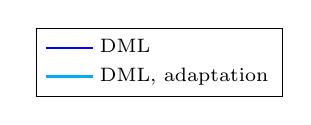
\begin{tikzpicture}[font=\scriptsize]

\begin{axis}[%
width=0.95092\figurewidth,
height=\figureheight,
at={(0\figurewidth,0\figureheight)},
scale only axis,
xmin=1,
xmax=50,
xlabel={Rank},
ymin=0,
ymax=1,
ylabel={Identification rate (\%)},
axis x line*=bottom,
axis y line*=left,
legend style={at={($ (0,1) + (+0.1cm,+0.1cm) $)},anchor=north west,align=left,legend cell align=left,draw=black},
xmajorgrids,
ymajorgrids,
grid style={dashed}
]
\addplot [color=blue,solid,line width=1.0pt]
  table[row sep=crcr]{%
1    0.1518987341772152\\
5    0.34810126582278483\\
10   0.47468354430379744\\
15   0.5474683544303798\\
20   0.5886075949367089\\
25   0.629746835443038\\
30   0.6613924050632911\\
35   0.680379746835443\\
40   0.7120253164556962\\
45   0.7183544303797469\\
50   0.7310126582278481\\
};
\addlegendentry{DML};

\addplot [color=cyan,solid,line width=1.0pt]
  table[row sep=crcr]{%
1    0.14556962025316456\\
5    0.3322784810126582\\
10   0.4873417721518987\\
15   0.5569620253164557\\
20   0.5917721518987342\\
25   0.6424050632911392\\
30   0.689873417721519\\
35   0.7025316455696202\\
40   0.7278481012658228\\
45   0.7531645569620253\\
50   0.7848101265822784\\
};
\addlegendentry{DML, adaptation};



\end{axis}
\end{tikzpicture}%
        \centering\small{(a) Whole CUHK $\rightarrow$ VIPeR}
        \label{fig:allcuhk_viper}
  
    &
        \setlength\figureheight{3.5cm}
        \setlength\figurewidth{3.5cm}
        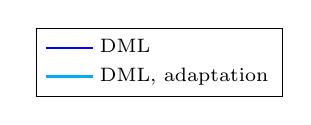
\begin{tikzpicture}[font=\scriptsize]

\begin{axis}[%
width=0.95092\figurewidth,
height=\figureheight,
at={(0\figurewidth,0\figureheight)},
scale only axis,
xmin=1,
xmax=50,
xlabel={Rank},
ymin=0,
ymax=1,
ylabel={Identification rate (\%)},
axis x line*=bottom,
axis y line*=left,
legend style={at={($ (0,1) + (+0.1cm,+0.1cm) $)},anchor=north west,align=left,legend cell align=left,draw=black},
xmajorgrids,
ymajorgrids,
grid style={dashed}
]
\addplot [color=blue,solid,line width=1.0pt]
  table[row sep=crcr]{%
1      0.126582278481 \\
5      0.303797468354 \\
10      0.414556962025 \\
15      0.490506329114 \\
20      0.550632911392 \\
25      0.613924050633 \\
30      0.651898734177 \\
35      0.686708860759 \\
40      0.708860759494 \\
45      0.75 \\
50      0.759493670886 \\
};
\addlegendentry{DML};

\addplot [color=cyan,solid,line width=1.0pt]
  table[row sep=crcr]{%
1      0.120253164557 \\
5      0.29746835443 \\
10      0.462025316456 \\
15      0.541139240506 \\
20      0.594936708861 \\
25      0.617088607595 \\
30      0.645569620253 \\
35      0.667721518987 \\
40      0.696202531646 \\
45      0.712025316456 \\
50      0.73417721519 \\
};
\addlegendentry{DML, adaptation};


\end{axis}
\end{tikzpicture}%
        \centering\small{(b) CUHK/p1 $\rightarrow$ VIPeR}
%        \label{fig:cuhk_p1_viper}
    &
        \setlength\figureheight{3.5cm}
        \setlength\figurewidth{3.5cm}
        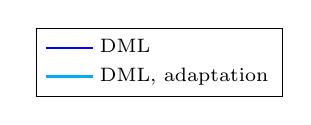
\begin{tikzpicture}[font=\scriptsize]

\begin{axis}[%
width=0.95092\figurewidth,
height=\figureheight,
at={(0\figurewidth,0\figureheight)},
scale only axis,
xmin=1,
xmax=50,
xlabel={Rank},
ymin=0,
ymax=1,
ylabel={Identification rate (\%)},
axis x line*=bottom,
axis y line*=left,
legend style={at={($ (0,1) + (+0.1cm,+0.1cm) $)},anchor=north west,align=left,legend cell align=left,draw=black},
xmajorgrids,
ymajorgrids,
grid style={dashed}
]
\addplot [color=blue,solid,line width=1.0pt]
  table[row sep=crcr]{%
1      0.0664556962025 \\
5      0.167721518987 \\
10      0.253164556962 \\
15      0.275316455696 \\
20      0.316455696203 \\
25      0.348101265823 \\
30      0.379746835443 \\
35      0.414556962025 \\
40      0.45253164557 \\
45      0.474683544304 \\
50      0.496835443038 \\
};
\addlegendentry{DML};

\addplot [color=cyan,solid,line width=1.0pt]
  table[row sep=crcr]{%
1      0.0632911392405 \\
5      0.161392405063 \\
10      0.259493670886 \\
15      0.338607594937 \\
20      0.389240506329 \\
25      0.417721518987 \\
30      0.439873417722 \\
35      0.471518987342 \\
40      0.496835443038 \\
45      0.518987341772 \\
50      0.53164556962 \\
};
\addlegendentry{DML, adaptation};


\end{axis}
\end{tikzpicture}%
        \centering\small{(c) PRID $\rightarrow$ VIPeR}
%        \label{fig:cuhk_p1_viper} \\    
 \end{tabular}
%  \caption{Results on VIPeR}
%  \label{fig:viper}
% \end{figure}%

% \begin{figure}[h]
% \centering
 \begin{tabular}{ p{5cm}  p{5cm}  p{5cm} }
        \setlength\figureheight{3.5cm}
        \setlength\figurewidth{4cm}
        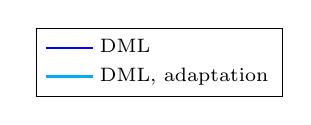
\begin{tikzpicture}[font=\scriptsize]

\begin{axis}[%
width=0.95092\figurewidth,
height=\figureheight,
at={(0\figurewidth,0\figureheight)},
scale only axis,
xmin=1,
xmax=50,
xlabel={Rank},
ymin=0,
ymax=1,
ylabel={Identification rate (\%)},
axis x line*=bottom,
axis y line*=left,
legend style={at={($ (0,1) + (+0.1cm,+0.1cm) $)},anchor=north west,align=left,legend cell align=left,draw=black},
xmajorgrids,
ymajorgrids,
grid style={dashed}
]
\addplot [color=blue,solid,line width=1.0pt]
  table[row sep=crcr]{%
1    0.08\\
5    0.13\\
10   0.22\\
15   0.27\\
20   0.31\\
25   0.35\\
30   0.4\\
35   0.41\\
40   0.41\\
45   0.43\\
50   0.44\\
};
\addlegendentry{DML};

\addplot [color=cyan,solid,line width=1.0pt]
  table[row sep=crcr]{%
1    0.07\\
5    0.19\\
10   0.27\\
15   0.32\\
20   0.35\\
25   0.37\\
30   0.39\\
35   0.41\\
40   0.43\\
45   0.45\\
50   0.45\\
};
\addlegendentry{DML, adaptation};


%[0.08, 0.13, 0.22, 0.27, 0.31, 0.35, 0.4, 0.41, 0.41, 0.43, 0.44]
%[0.07, 0.19, 0.27, 0.32, 0.35, 0.37, 0.39, 0.41, 0.43, 0.45, 0.45]

%
\end{axis}
\end{tikzpicture}%





        \centering\small{(d) Whole CUHK $\rightarrow$ PRID}
        \label{fig:allcuhk_prid}
    &
        \setlength\figureheight{3.5cm}
        \setlength\figurewidth{4cm}
        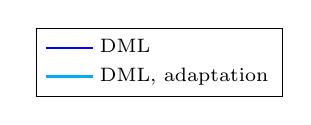
\begin{tikzpicture}[font=\scriptsize]

\begin{axis}[%
width=0.95092\figurewidth,
height=\figureheight,
at={(0\figurewidth,0\figureheight)},
scale only axis,
xmin=1,
xmax=50,
xlabel={Rank},
ymin=0,
ymax=1,
ylabel={Identification rate (\%)},
axis x line*=bottom,
axis y line*=left,
legend style={at={($ (0,1) + (+0.1cm,+0.1cm) $)},anchor=north west,align=left,legend cell align=left,draw=black},
xmajorgrids,
ymajorgrids,
grid style={dashed}
]
\addplot [color=blue,solid,line width=1.0pt]
  table[row sep=crcr]{%
1      0.04 \\
5      0.08 \\
10      0.15 \\
15      0.22 \\
20      0.25 \\
25      0.3 \\
30      0.32 \\
35      0.36 \\
40      0.39 \\
45      0.41 \\
50      0.44 \\
};
\addlegendentry{DML};

\addplot [color=cyan,solid,line width=1.0pt]
  table[row sep=crcr]{%
1      0.06 \\
5      0.16 \\
10      0.21 \\
15      0.27 \\
20      0.31 \\
25      0.36 \\
30      0.39 \\
35      0.41 \\
40      0.41 \\
45      0.42 \\
50      0.43 \\
};
\addlegendentry{DML, adaptation};


\end{axis}
\end{tikzpicture}%
        \centering\small{(e) CUHK/p1 $\rightarrow$ PRID}
        \label{fig:cuhk_p1_prid}
    &
       \setlength\figureheight{3.5cm}
       \setlength\figurewidth{4cm}
       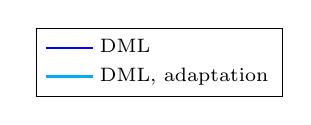
\begin{tikzpicture}[font=\scriptsize]

\begin{axis}[%
width=0.95092\figurewidth,
height=\figureheight,
at={(0\figurewidth,0\figureheight)},
scale only axis,
xmin=1,
xmax=50,
xlabel={Rank},
ymin=0,
ymax=1,
ylabel={Identification rate (\%)},
axis x line*=bottom,
axis y line*=left,
legend style={at={($ (0,1) + (+0.1cm,+0.1cm) $)},anchor=north west,align=left,legend cell align=left,draw=black},
xmajorgrids,
ymajorgrids,
grid style={dashed}
]
\addplot [color=blue,solid,line width=1.0pt]
  table[row sep=crcr]{%
1      0.08 \\
5      0.15 \\
10      0.19 \\
15      0.25 \\
20      0.28 \\
25      0.34 \\
30      0.35 \\
35      0.36 \\
40      0.39 \\
45      0.4 \\
50      0.41 \\
};
\addlegendentry{DML};

\addplot [color=cyan,solid,line width=1.0pt]
  table[row sep=crcr]{%
1      0.07 \\
5      0.19 \\
10      0.25 \\
15      0.27 \\
20      0.31 \\
25      0.36 \\
30      0.39 \\
35      0.42 \\
40      0.42 \\
45      0.46 \\
50      0.47 \\
};
\addlegendentry{DML, adaptation};


\end{axis}
\end{tikzpicture}%
        \centering\small{(f) VIPeR $\rightarrow$ PRID}
        \label{fig:viper_prid}  \\    
 \end{tabular}
%  \caption{Results on PRID}
%  \label{fig:prid}
% \end{figure}


% \begin{figure}[h]
% \centering
 \begin{tabular}{ p{5cm}  p{5cm}}
        \setlength\figureheight{3.5cm}
        \setlength\figurewidth{4cm}
        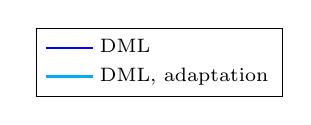
\begin{tikzpicture}[font=\scriptsize]

\begin{axis}[%
width=0.95092\figurewidth,
height=\figureheight,
at={(0\figurewidth,0\figureheight)},
scale only axis,
xmin=1,
xmax=50,
xlabel={Rank},
ymin=0,
ymax=1,
ylabel={Identification rate (\%)},
axis x line*=bottom,
axis y line*=left,
legend style={at={($ (0,1) + (+0.1cm,+0.1cm) $)},anchor=north west,align=left,legend cell align=left,draw=black},
xmajorgrids,
ymajorgrids,
grid style={dashed}
]
\addplot [color=blue,solid,line width=1.0pt]
  table[row sep=crcr]{%
1      0.109053497942 \\
5      0.265432098765 \\
10      0.366255144033 \\
15      0.407407407407 \\
20      0.465020576132 \\
25      0.491769547325 \\
30      0.510288065844 \\
35      0.541152263374 \\
40      0.572016460905 \\
45      0.59670781893 \\
50      0.617283950617 \\
};
\addlegendentry{DML};

\addplot [color=cyan,solid,line width=1.0pt]
  table[row sep=crcr]{%
1      0.125514403292 \\
5      0.253086419753 \\
10      0.366255144033 \\
15      0.440329218107 \\
20      0.5 \\
25      0.5329218107 \\
30      0.572016460905 \\
35      0.594650205761 \\
40      0.617283950617 \\
45      0.650205761317 \\
50      0.668724279835 \\
};
\addlegendentry{DML, adaptation};


\end{axis}
\end{tikzpicture}%
        \centering\small{(g) VIPeR $\rightarrow$ CUHK/p1}
        \label{fig:viper_cuhk_p1}
    &
        \setlength\figureheight{3.5cm}
        \setlength\figurewidth{4cm}
        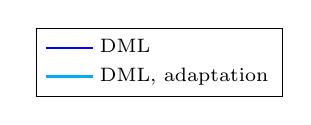
\begin{tikzpicture}[font=\scriptsize]

\begin{axis}[%
width=0.95092\figurewidth,
height=\figureheight,
at={(0\figurewidth,0\figureheight)},
scale only axis,
xmin=1,
xmax=50,
xlabel={Rank},
ymin=0,
ymax=1,
ylabel={Identification rate (\%)},
axis x line*=bottom,
axis y line*=left,
legend style={at={($ (0,1) + (+0.1cm,+0.1cm) $)},anchor=north west,align=left,legend cell align=left,draw=black},
xmajorgrids,
ymajorgrids,
grid style={dashed}
]
\addplot [color=blue,solid,line width=1.0pt]
  table[row sep=crcr]{%
1      0.0569620253165 \\
5      0.139240506329 \\
10      0.212025316456 \\
15      0.284810126582 \\
20      0.316455696203 \\
25      0.344936708861 \\
30      0.370253164557 \\
35      0.389240506329 \\
40      0.414556962025 \\
45      0.443037974684 \\
50      0.465189873418 \\
};
\addlegendentry{DML};

\addplot [color=cyan,solid,line width=1.0pt]
  table[row sep=crcr]{%
1      0.0843621399177 \\
5      0.191358024691 \\
10      0.263374485597 \\
15      0.316872427984 \\
20      0.347736625514 \\
25      0.395061728395 \\
30      0.432098765432 \\
35      0.471193415638 \\
40      0.504115226337 \\
45      0.5329218107 \\
50      0.553497942387 \\
};
\addlegendentry{DML, adaptation};


\end{axis}
\end{tikzpicture}%
        \centering\small{(h) PRID $\rightarrow$ CUHK/p1}
        \label{fig:prid_cuhk_p1}
  \\    
  \end{tabular}
  \caption{Results on VIPeR, PRID and CUHK/p1 with and without domain-adversarial learning. Across the eight domain pairs domain-adversarial learning improves re-identification accuracy. For some domain pairs the improvement is considerable.}
  \label{fig:adaptresults}
\end{figure}

Figure \ref{fig:adaptresults} shows results in the form of CMC-curves for eight pairs of data sets. Depending on the hardness of the annotation problem we trained either for 50,000 iterations (CUHK/p1 $\rightarrow$ VIPeR, VIPeR $\rightarrow$ CUHK/p1, PRID $\rightarrow$ VIPeR) or for 20,000 iterations (the other five pairs). 

\begin{figure*}
\centering
\begin{tabular}{c c}
\includegraphics[height=7cm, width=7cm]{./Chapters/gradrev/figures/reid_adapt_results/viper_cuhkp1_zc.png}&
\includegraphics[height=7cm, width=7cm]{./Chapters/gradrev/figures/reid_adapt_results/viper_cuhkp1_da.png}\\
\small{(a) DML}&
\small{(b) DML, adaptation}\\
\end{tabular}
\caption{The effect of adaptation shown by t-SNE visualizations of source and target domains descriptors in a VIPeR $\rightarrow$ CUHK/p1 experiment pair. VIPeR is depicted with \textit{green} and CUHK/p1 - with \textit{red}. As in the image classification case, domain-adversarial learning ensures a closer match between the source and the target distributions. }
\label{fig:reidtsne}
\end{figure*}


After the sufficient number of iterations, domain-adversarial training consistently improves the performance of re-identification. For the pairs that involve PRID data set, which is more dissimilar to the other two data sets, the improvement is considerable. Overall, this demonstrates the applicability of the domain-adversarial learning beyond classification problems.

Figure \ref{fig:reidtsne} further demonstrates the effect of adaptation on the distributions of the learned descriptors in the source and in target sets in VIPeR $\rightarrow$ CUHK/p1 experiments, where domain adversarial learning once again achieves better intermixing of the two domains.


\section{Conclusion}

The paper proposes a new approach to domain adaptation of feed-forward neural networks, which allows large-scale training based on large amount of annotated data in the source domain and large amount of unannotated data in the target domain. Similarly to many previous shallow and deep DA techniques, the adaptation is achieved through aligning the distributions of features across the two domains. However, unlike previous approaches, the alignment is accomplished through standard backpropagation training.

The approach is motivated and supported by the domain adaptation theory of \citet{BenDavid-NIPS06,BenDavid-MLJ2010}. 
The main idea behind DANN is to enjoin the network hidden layer to learn a representation which is predictive of the source example labels, but uninformative about the domain of the input (source or target). 
We implement this new approach within both shallow and deep feed-forward architectures. The latter allows simple implementation within virtually any deep learning package through the introduction of a simple gradient reversal layer. 
We have shown that our approach is flexible and achieves state-of-the-art results on a variety of benchmark in domain adaptation, namely for sentiment analysis and image classification tasks. 

A convenient aspect of our approach is that the domain adaptation component can be added to almost any neural network architecture that is trainable with backpropagation. Towards this end, We have demonstrated experimentally that the approach is not confined to classification tasks but can be used in other feed-forward architectures, e.g.\ for descriptor learning for person re-identification.


\section{Motivation}




%problem intuition
In many practical cases, we do not have access to a sufficient amount of labeled training data for supervised learning. This problem is especially critical for learning deep neural networks that often incorporate millions of parameters. However, it is often the case that the training data are available, and the labeling corresponds to the task of interest, but the data differ from those that our predictor will encounter during test time. Such difference between the training data (source) and possible test data (target) is referred to as a \textit{domain shift} or \textit{covariate shift}. In more detail, this means that the source and target data share the same feature space, and only their marginal distributions are assumed to be different. 

%example
One important example of the described situation is training on synthetic images that can be generated automatically (\eg{} by 3D rendering systems). This is a particularly practical use case, as collecting the necessary amount of analogous real data and its labeling may be very time-consuming. 
In this way, the ability to overcome the domain shift between the available synthetic and target data is crucial for the final performance of the predictor. 

%notation?

%how others solve the problem
Although there exist many powerful methods for domain adaptation \cite{huang2007correcting, pan2008transfer, pan2011domain,baktashmotlagh2013unsupervised,gong2012geodesic,gong2013connecting}, they most often work for the fixed feature representations and therefore are limited by these representations. %Most often, such methods cannot be naturally incorporated to the process of learning deep neural network. 

Several works have also approached domain adaptation in the framework of deep learning. \cite{glorot2011domain} and \cite{chopra2013dlid} train the denoising autoencoders on a mixture of data from the two domains to get the domain-invariant feature extractors. The task-specific training is performed as the second step (although, at this step, \cite{chopra2013dlid} finetunes both task-specific neural network and the pre-trained feature extractor using the task-specific loss). In contrast to \cite{glorot2011domain} and \cite{chopra2013dlid}, \cite{LongC0J15} and \cite{tzeng2014deep} apply a special loss function (based on Maximum Mean Discrepancy) to pull the two domains closer. Such an objective can be optimized simultaneously with the task-specific loss. This allows to learn the representations that are useful for the task of interest and at the same time are domain-invariant.

%how it is suggested in the paper
A new way of deep domain adaptation is suggested in this chapter. Like in the works of \cite{LongC0J15} and \cite{tzeng2014deep}, the goal is to incorporate domain adaptation into the process of training a classification neural network, so that the learned deep representations are 
\begin{itemize}
    \item discriminative (\ie{} useful for classification),
    \item  domain-invariant (\ie{} the feature distributions are close for the two domains)
\end{itemize}. 
 This is achieved by jointly optimizing the two deep discriminative classifiers:  \begin{itemize}
     \item the task-specific label predictor,
     \item the domain classifier that discriminates between the source and the target domains.
 \end{itemize}
The parameters of these two classifiers are optimized in order to minimize their error on the training set. What provides discriminativeness and domain-invariance of the learned features is that these features are optimized simultaneously to 
\begin{itemize} 
    \item minimize the error of the task-specific classifier, 
    \item maximize the error of the domain classifier. 
 \end{itemize}

Such combination of objectives can be optimized for feed-forward networks using standard backpropagation algorithm based on stochastic gradient descent. To perform a domain-adversarial training of feature representation, the gradient reversal layer is introduced. No labeling is needed for the target domain, so the approach is suitable for \textit{unsupervised domain adaptation}.

It should be noted that an idea related to ours is described in \citep{Goodfellow14}. While their goal is quite different (building generative deep networks that can synthesize samples), the way they measure and minimize the discrepancy between the distribution of the training data and the distribution of the synthesized data is very similar to the way our architecture measures and minimizes the discrepancy between feature distributions for the two domains. %Moreover, the authors mention the problem  of saturating sigmoids which may arise at the early stages of training due to the significant dissimilarity of the domains. The technique they use to circumvent this issue (the ``adversarial'' part of the gradient is replaced by a gradient computed with respect to a suitable cost) is directly applicable to our method. 

First, the described approach is evaluated for an image classification task. This chapter includes the results only for digit classification (on the MNIST dataset \citep{LeCun98}). The extensive evaluation for many other classifications tasks can be found in the corresponding publication [\cite{ganin2016domain}].

Domain-adversarial training is also demonstrated to be applicable to person re-identification. Several publicly available datasets are considered as different domains. 
To adapt the described approach to person re-identification, we consider a \textit{descriptor predictor} trained with a Siamese-like loss instead of the label predictor trained with a classification loss. In a series of experiments, we demonstrate that domain-adversarial learning can improve cross-dataset re-identification considerably. 




%mention goodfellow, CycleGAN, about the assumption of having to adapt last layers.


\section{Domain Adaptation}
\label{section:DA_theory}

We consider classification tasks where $\Xcal$ is the input space and $\Ycal=\{0,1,\ldots,L{-}1\}$ is the set of $L$ possible labels.
Moreover, we have two different distributions over $\Xcal\!\times\! \Ycal$, called the {\it source domain} $\DS$ and the {\it target domain} $\DT$.
An \emph{unsupervised domain adaptation} learning algorithm is then provided with a {\it labeled source sample} $S$ drawn {\it i.i.d.} from $\DS$, and an {\it unlabeled target sample} $T$ drawn {\it i.i.d.} from $\DTX$, where $\DTX$ is the marginal distribution of $\DT$ over~$\Xcal$.
%\footnote{For simplicity, we consider through this paper that the source sample $S$ and the target sample $T$ are of equal size~$m$. It is easy to generalize the results for the case where $|S|\neq|T|$.}
\begin{equation*}
S = \{(\xb_i,\ys_i)\}_{i=1}^{n} \sim (\DS)^n 
\,; \quad
%\quad\mbox{and}\quad
T = \{\xb_i\}_{i=n+1}^{N} \sim (\DTX)^{n'},
\end{equation*}
with $N=n+n'$ being the total number of samples. 
%
The goal of the learning algorithm is to build a classifier $\eta:\Xcal\to\Ycal$ with a low \emph{target~risk}
\begin{equation*}
\RDT(\eta) \ \eqdef \Pr_{(\xb,\yt) \sim \DT} \Big(\eta(\xb) \neq \yt\Big)\,,
\end{equation*}
while having no information about the labels of $\DT$.

% \bigskip
% \indent\textbf{Domain Divergence}
% %\subsection{Domain Divergence}

% To tackle the challenging domain adaptation task, many  approaches bound the target error by the sum of the source error and a notion of distance between the source and the target distributions. These methods are intuitively justified by a simple assumption: the source risk is expected to be a good indicator of the target risk when both distributions are similar. Several notions of distance have been proposed for domain adaptation~\citep{BenDavid-NIPS06,Mansour-COLT09,MansourMR09,pbda}.
% In this paper, we focus on the $\Hcal$-divergence used by ~\citet{BenDavid-NIPS06}, and based on the earlier work of~\citet{kifer-2004}. Note that we assume in definition~\ref{def:Hdiv} below that the hypothesis class $\Hcal$ is a (discrete or continuous) set of binary classifiers $\eta:\Xcal\to\{0,1\}$.\footnote{As mentioned by \citet{BenDavid-NIPS06}, the same analysis holds for multiclass setting. However, to obtain the same results when $|Y|>2$, one should assume that $\Hcal$ is a symmetrical hypothesis class. That is, for all $h\in\Hcal$ and any permutation of labels $c:Y\to Y$, we have $c(h)\in \Hcal$. Note that this is the case for most commonly used neural network architectures.}
% \begin{definition}[\citealp{BenDavid-NIPS06, kifer-2004}] \label{def:Hdiv}
% Given two domain distributions $\DSX$ and $\DTX$ over~$\Xcal$, and a hypothesis class~$\Hcal$, the \emph{$\Hcal$-divergence} between $\DSX$ and $\DTX$ is
% \begin{eqnarray*}
% d_\Hcal(\DSX,\DTX)  &\eqdef & 
% 2 \,\sup_{\eta\in\Hcal} \,\bigg|\, 
% \Pr_{\xb \sim \DSX} \big[\eta(\xb) = 1\big] - 
% \Pr_{\xb \sim \DTX} \big[\eta(\xb) = 1\big]\,
% \bigg|\,.
% \end{eqnarray*}
% \end{definition}

% That is, the $\Hcal$-divergence relies on the capacity of the hypothesis class $\Hcal$ to distinguish between examples generated by $\DSX$ from examples generated by $\DTX$.
% \citet{BenDavid-NIPS06} proved that, for a symmetric hypothesis class $\Hcal$, one can compute the \emph{empirical $\Hcal$-divergence} between two samples $S\sim(\DSX)^n$ and  $T\sim(\DTX)^{n'}$ by computing
% \begin{eqnarray} \label{eq:Hdiv_empirique}
%  \hat{d}_\Hcal(S,T) & \eqdef & 
%  2\,\Bigg( 1 - \min_{\eta\in\Hcal} \bigg[
% \frac{1}{n} \sum_{i=1}^n I[\eta(\xb_i)\!=\!0] + \frac{1}{n'} \sum_{i=n+1}^{N} I[\eta(\xb_i)\!=\!1]
% \bigg] \Bigg)\,,
% \end{eqnarray}
% where $I[a]$ is the indicator function which is $1$ if predicate $a$ is true, and $0$ otherwise.

% \bigskip
% \indent\textbf{Proxy Distance}
% %\subsection{Proxy Distance}
% \label{section:PAD}

% %\citet{BenDavid-NIPS06,BenDavid-MLJ2010}
% \citet{BenDavid-NIPS06}
% suggested that, even if it is generally hard to compute $\hat{d}_\Hcal(S,T)$ exactly (\eg, when $\Hcal$ is the space of linear classifiers on $\Xcal$), we can easily approximate it by running a learning algorithm on the problem of discriminating between source and target examples. To do so, we construct a new dataset
% \begin{equation}\label{eq:U}
% U \ =\ \{(\xb_i, 0)\}_{i=1}^n \cup \{(\xb_i, 1)\}_{i=n+1}^{N}\,,
% \end{equation}
% where the examples of the source sample are labeled $0$ and the examples of the target sample are labeled $1$. Then, the risk of the classifier trained on the new dataset $U$ approximates the ``$\min$'' part of Equation~\eqref{eq:Hdiv_empirique}. 
% Given a generalization error~$\epsilon$ on the problem of discriminating between source and target examples, the $\Hcal$-divergence is then approximated by
% \begin{equation} \label{eq:PAD}
% \hat{d}_\Acal \ = \ 2\,(1-2\epsilon)\,.
% \end{equation}
% In \citep{BenDavid-NIPS06}, the value $\hat{d}_\Acal$ is called the \emph{Proxy $\Acal$-distance} (PAD). The \emph{$\Acal$-distance}
% being defined as 
% $
% d_\Acal(\DSX,\DTX)  \eqdef 
% 2 \,\sup_{A\in\Acal} \,\big|\, 
% \Pr_{\DSX} (A) - 
% \Pr_{\DTX} (A)\,
% \big|
% $,
% where $\Acal$ is a subset of $\Xcal$. Note that, by choosing $\Acal = \{A_\eta | \eta \in \Hcal\}$, with $A_\eta$ the set represented by the characteristic function $\eta$, the $\Acal$-distance and the $\Hcal$-divergence of Definition~\ref{def:Hdiv} are identical.

% In the classification experiments section of this chapter, we compute the PAD value following the approach of \citep{glorot2011domain}, \ie, we train either a linear SVM or a deeper MLP classifier on a subset of $U$ (Equation~\ref{eq:U}), and we use the obtained classifier error on the other subset as the value of~$\epsilon$ in Equation~\eqref{eq:PAD}. 
% %More details and illustrations of the linear SVM case are provided in Section~\ref{section:PAD_experiments}.

% \bigskip
% \indent\textbf{Generalization Bound on the Target Risk}

% %\subsection{Generalization Bound on the Target Risk}
% The work of \citet{BenDavid-NIPS06} also showed that the $\Hcal$-divergence $d_\Hcal(\DSX,\DTX)$ is upper bounded by its empirical estimate $\hat{d}_\Hcal(S,T)$ plus a constant complexity term that depends on the \emph{VC dimension} of $\Hcal$ and the size of samples $S$ and $T$. By combining this result with a similar bound on the source risk, the following theorem is obtained.
% \begin{theorem}[\citealp{BenDavid-NIPS06}] 
% \label{thm:RDT_bound}
% Let $\Hcal$ be a hypothesis class of VC dimension $d$.
% With probability $1-\delta$ over the choice of samples $S\sim (\DS)^n$ and $T\sim (\DTX)^{n}$, for every $\eta\in\Hcal$:
% \begin{eqnarray*}
% \RDT(\eta) &\leq&  
% \RS(\eta) +  \sqrt{\frac{4}{n}\left( d \log\tfrac{2e\, n}{d}+  \log\tfrac{4}{\delta}\right) } 
% +\hat{d}_\Hcal(S,T) + 4\sqrt{ \frac{1}{n}\left(d \log\tfrac{2 n}{d}+  \log\tfrac{4}{\delta}\right) }
% + \beta\,,
% \end{eqnarray*}
% with $\beta \geq {\displaystyle\inf_{\eta^*\in\Hcal}} \left[ \RDS(\eta^*) + \RDT(\eta^*) \right]$\,, 
% and 
% «\begin{equation*}
% \RS(\eta) \ =\ \frac{1}{n}\dsum_{i=1}^m I\left[\eta(\xb_i) \neq \ys_i\right]
% \end{equation*}
% is the {empirical source~risk}.
% %\begin{equation*}
% %\RS(\eta) \ \eqdef \ \frac{1}{m} \sum_{(\xb,y)\in S} I[\eta(\xb) = y]\,.
% %\end{equation*}
% \end{theorem}
% The previous result tells us that $\RDT(\eta)$ can be low only when the $\beta$ term is low, \ie, only when there exists a classifier that can achieve a low risk on both distributions. It also tells us that, to find a classifier with a small $\RDT(\eta)$ in a given class of fixed VC dimension, the learning algorithm should minimize (in that class) a trade-off between the source risk $\RS(\eta)$ and the empirical $\Hcal$-divergence $\hat{d}_\Hcal(S,T)$.  
% As pointed-out by~\citet{BenDavid-NIPS06}, a strategy to control the $\Hcal$-divergence is to find a representation of the examples where both the source and the target domain are as indistinguishable as possible. Under such a representation, a hypothesis with a low source risk will, according to Theorem~\ref{thm:RDT_bound}, perform well on the target data.  
% In this paper, we present an algorithm that directly exploits this idea.


\section{Domain-Adversarial Neural Networks (DANN)}
\label{section:dann}

%An original aspect of our approach is to explicitly implement the idea exhibited by Theorem~\ref{thm:RDT_bound} 
%into a neural network classifier.
To learn a
model that can generalize well from one domain to another, we ensure that
the internal representation of the neural network contains no discriminative information about the origin of the input (source or target), while preserving a low risk on the source (labeled) examples.

In this section, we detail the proposed approach for incorporating a ``domain adaptation component'' to neural networks.
%In Subsection~\ref{section:shallow_dann}, we start by developing the idea for the simplest possible case, \ie,  a single hidden layer, fully connected neural network. We then describe how to generalize the approach to arbitrary  (deep) network architectures. 




 \begin{figure*}[t]
 \centering
 \includegraphics[width=0.85\textwidth]{Chapters/gradrev/figures/deepDA2_c.pdf}
 \caption{The {\bf proposed architecture} includes a deep {\em feature extractor} (green) and a deep {\em label predictor} (blue), which together form a standard feed-forward architecture. Unsupervised domain adaptation is achieved by adding a {\em domain classifier} (red) connected to the feature extractor via a {\em gradient reversal layer} that multiplies the gradient by a certain negative constant during the backpropagation-based training. Otherwise, the training proceeds standardly and minimizes the label prediction loss (for source examples) and the domain classification loss (for all samples). Gradient reversal ensures that the feature distributions over the two domains are made similar (as indistinguishable as possible for the domain classifier), thus resulting in the domain-invariant features.\vspace{-2mm}}
 \label{fig:arch}
 \end{figure*}
 

%\bigskip
%\indent\textbf{Generalization to Arbitrary Architectures}


%\subsection{Generalization to Arbitrary Architectures}
%\label{section:deep_DANN}
%
%We now detail the proposed model for the domain adaptation. We assume that the model works with input samples $\x \in X$, where $X$ is some input space and certain labels (output) $y$ from the label space $Y$. Below, we assume classification problems where $Y$ is a finite set ($Y=\{1,2,\dots L\}$), however our approach is generic and can handle any output label space that other deep feed-forward models can handle. We further assume that there exist two distributions $\S(x,y)$ and $\T(x,y)$ on $X\otimes Y$, which will be referred to as the source distribution and the target distribution (or the source domain and the target domain). Both distributions are assumed complex and unknown, and furthermore similar but different (in other words, $\S$ is ``shifted'' from $\T$ by some {\em domain shift}). 

%Our ultimate goal is to be able to predict labels $y$ given the input $\x$ for the target distribution. At training time, we have an access to a large set of training samples $\{\x_1,\x_2,\dots,\x_N\}$ from both the source and the target domains distributed according to the marginal distributions $\S(\x)$ and $\T(\x)$. We denote with $d_i$ the binary variable ({\em domain label}) for the $i$-th example, which indicates whether $x_i$ come from the source distribution ($\x_i{\sim}\S(\x)$ if $d_i{=}0$) or from the target distribution ($\x_i{\sim}\T(\x)$ if $d_i{=}1$). For the examples from the source distribution ($d_i{=}0$) the corresponding labels $y_i \in Y$ are known at training time. For the examples from the target domains, we do not know the labels at training time, and we want to predict such labels at test time.

For illustration purposes, we've so far focused on the case of a single hidden layer DANN. However, it is straightforward to generalize to other sophisticated architectures, which might be more appropriate for the data at hand. For example,  deep convolutional neural networks are well known for being state-of-the-art models for learning discriminative features of images~\citep{Krizhevsky12}.

Let us now use a more general notation for the different components of DANN. Namely, let $G_f(\cdot; \tf)$ be the $D$-dimensional neural network feature extractor, with parameters $\tf$. Also, let $G_y(\cdot; \ty)$ be the part of DANN that computes the network's label prediction output layer, with parameters $\ty$, while $G_d(\cdot;\td)$ now corresponds to the computation of the domain prediction output of the network, with parameters $\td$.
%Note that for preserving the theoretical guarantees of Theorem~\ref{thm:RDT_bound}, the hypothesis class $\Hcal_d$ generated by the domain prediction component $G_d$ should include the hypothesis class $\Hcal_y$ generated by the label prediction component $G_y$. Thus, $\Hcal_y\subseteq\Hcal_d$.

We will note the prediction loss and the domain loss respectively by
\begin{eqnarray*}
\Lcal_y^i(\tf, \ty)&=& \Lcal_{y} \big( G_y(G_f(\xb_i; \tf); \ty), y_i\big)\,,\\ 
\Lcal_{d}^i(\tf, \td)&=& \Lcal_{d} \big( G_d(G_f(\xb_i; \tf); \td), d_i)\,.
\end{eqnarray*}
% :)
Training DANN then consists in optimizing
\begin{eqnarray}
E (\tf,\ty,\td)
= \frac{1}{n}\sum_{i=1}^n \Lcal_y^i(\tf,\ty)
- \lambda \,\Big(\frac{1}{n} \sum_{i=1}^{n} \Lcal_{d}^i(\tf, \td)  + \frac{1}{n'} \sum_{\mathclap{i=n+1}}^{N} \Lcal_{d}^i(\tf, \td )\Big),
\label{eqn:global_gen}
\end{eqnarray}
by finding the saddle point $\htf,\hty,\htd$ such that
\begin{eqnarray}
(\htf,\hty) &=& \argmin_{\tf,\ty}\, E(\tf,\ty,\htd)\,,\label{eq:opt1}\\\label{eq:opt2}
\htd &=& \argmax_\td \, E(\htf,\hty, \td)\,.
\end{eqnarray}




As suggested previously, a saddle point defined by Equations~(\ref{eq:opt1}-\ref{eq:opt2}) can be found as a stationary point of the following gradient updates:
{\allowdisplaybreaks[4]
\begin{align}
\tf \quad &\longleftarrow \quad \tf \;-\; \mu \left(\frac{\partial \Lcal_y^i}{\partial \tf}-\lambda\frac{\partial \Lcal_d^i}{\partial \tf} \right), \label{eq:upd1}\\
\ty \quad &\longleftarrow \qquad \ty \;-\; \mu \frac{\partial \Lcal_y^i}{\partial \ty}\,,\label{eq:upd2}\\
\td \quad &\longleftarrow \qquad \td \;-\; \mu \lambda \frac{\partial \Lcal_d^i}{\partial \td}\,, \label{eq:upd3}
\end{align}
}where $\mu$ is the learning rate. We use stochastic estimates of these gradients, by sampling examples from the dataset.

The updates of Equations~(\ref{eq:upd1}-\ref{eq:upd3}) are very similar to stochastic gradient descent (SGD) updates for a feed-forward deep model that comprises feature extractor fed into the label predictor and into the domain classifier (with loss weighted by $\lambda$). The only difference is that in \eq{upd1}, the gradients from the class and domain predictors are subtracted, instead of being summed (the difference is important, as otherwise SGD would try to make features dissimilar across domains in order to minimize the domain classification loss). Since SGD, and its many variants, is the main learning algorithm implemented in most libraries for deep learning, it would be convenient to frame an implementation of our stochastic saddle point procedure as SGD.

Fortunately, such a reduction can be accomplished by introducing a special \emph{gradient reversal layer} (GRL), defined as follows. The gradient reversal layer has no parameters associated with it.
%(apart from the meta-parameter $\lambda$, which is not updated by backpropagation). 
During the forward propagation, the GRL acts as an identity transformation. During the backpropagation however, the GRL takes the gradient from the subsequent level and changes its sign, \ie multiplies it by $-1$, before passing it to the preceding layer. Implementing such a layer using existing object-oriented packages for deep learning is simple, requiring only to define procedures for the forward propagation (identity transformation), and backpropagation (multiplying by $-1$). The layer requires no parameter update. 

The GRL as defined above is inserted between the feature extractor $G_f$ and the domain classifier $G_d$, resulting in the architecture depicted in \fig{arch}. As the backpropagation process passes through the GRL, the partial derivatives of the loss that is downstream the GRL (\ie, $\Lcal_d$) w.r.t.\ the layer parameters that are upstream the GRL (\ie, $\tf$) get multiplied by $-1$, \ie, $\frac{\partial \Lcal_d}{\partial \tf}$ is effectively replaced with $-\frac{\partial \Lcal_d}{\partial \tf}$. Therefore, running SGD in the resulting model implements the updates of Equations~(\ref{eq:upd1}-\ref{eq:upd3}) and converges to a saddle point of Equation~\eqref{eqn:global_gen}.

Mathematically, we can formally treat the gradient reversal layer as a ``pseudo-function'' ${\cal R}(\x)$ defined by two (incompatible) equations describing its forward and backpropagation behaviour:
\begin{align}
{\cal R}(\x) = \x\,,\\
\frac{d{\cal R}}{d\x} = -\mathbf{I}\,,
\end{align}
where $\mathbf{I}$ is an identity matrix.
We can then define the objective ``pseudo-function'' of $(\tf,\ty,\td)$ that is being optimized by the stochastic gradient descent within our method:
\begin{eqnarray}
&&\tilde E (\tf,\ty,\td) = \! \frac{1}{n}\sum_{i=1}^n \Lcal_y\left( \strut G_y(G_f(\x_i;\tf);\ty), y_i\right)\label{eq:pseudoobj}\\
&&~~~- \lambda \,\Big(\frac{1}{n} \sum_{i=1}^{n} \Lcal_d \left( \strut G_d({\cal R}(G_f(\x_i;\tf));\td), d_i\right) + \frac{1}{n'} \sum_{\mathclap{i=n+1}}^{N} \Lcal_d \left( \strut G_d({\cal R}(G_f(\x_i;\tf));\td), d_i\right) \Big)\,.\nonumber
\end{eqnarray}

Running updates (\ref{eq:upd1}-\ref{eq:upd3}) can then be implemented as doing SGD for \eq{pseudoobj} and leads to the emergence of features that are domain-invariant and discriminative at the same time. After the learning, the label predictor $G_y(G_f(\x;\tf);\ty)$ can be used to predict labels for samples from the target domain (as well as from the source domain).


\section{Experiments}
\bigskip\indent\textbf{Experiments with deep networks on image classification}\\
%\bigskip
%\indent\textbf{Experiments with Deep Networks on Image %Classification}


\label{sect:experiments}

\begin{figure*}
  \centering
  \setlength{\tabcolsep}{0pt}
  \setlength\figurewidth{0.05\textwidth}
  \renewcommand{\example}[1]{\raisebox{-.4\height}{\includegraphics[width=\figurewidth]{Chapters/gradrev/figures/domains_examples/#1}}}
  \begin{sc}
  \begin{small}
  \begin{tabular}{r@{\hskip 0.5cm} ccc c@{\hskip 0.4cm} ccc c@{\hskip 0.4cm} ccc c@{\hskip 0.4cm} ccc}
    &
    \multicolumn{3}{c}{MNIST} & &
    % \multicolumn{3}{c}{Syn Numbers} & &
    % \multicolumn{3}{c}{SVHN} & &
    % \multicolumn{3}{c}{Syn Signs}
    \\
    
    Source &
    \example{mnist_0.png} &
    \example{mnist_1.png} &
    \example{mnist_3.png} & &
    
    % \example{syn_0.png} &
    % \example{syn_1.png} &
    % \example{syn_2.png} & &
    
    % \example{svhn_3.png} &
    % \example{svhn_4.png} &
    % \example{svhn_5.png} & &
    
    % \example{synsgn_3.png} &
    % \example{synsgn_4.png} &
    % \example{synsgn_5.png}
    \\
    
    Target &
    \example{mnisti_0.png} &
    \example{mnisti_1.png} &
    \example{mnisti_2.png} & &
    
    % \example{svhn_0.png} &
    % \example{svhn_1.png} &
    % \example{svhn_2.png} & &
    
    % \example{mnist_4.png} &
    % \example{mnist_5.png} &
    % \example{mnist_6.png} & &
    
    % \example{gtsrb_2.png} &
    % \example{gtsrb_3.png} &
    % \example{gtsrb_4.png}
    \\
    
    &
    \multicolumn{3}{c}{\rule{0pt}{0.35cm} MNIST-M} & &
    % \multicolumn{3}{c}{SVHN} & &
    % \multicolumn{3}{c}{MNIST} & &
    % \multicolumn{3}{c}{GTSRB}
    \\
  \end{tabular}
  \end{small}
  \end{sc}
  \caption{Examples of domain pairs used in the experiments. See \sect{exper_quant} for details.}
  \label{fig:exper_domains_examples}
\end{figure*}

\begin{table*}[t]
\centering
    \begin{small}
      \begin{sc}
        \renewcommand{\arraystretch}{1.3}
        \rowcolors{2}{black!10}{}
        \begin{tabular}{l r | c c c c}
          \hline
          \multirow{2}{*}{Method} & {\scriptsize Source} & MNIST \\ %& Syn Numbers & SVHN & Syn Signs \\
          & {\scriptsize Target} & MNIST-M \\ % & SVHN & MNIST & GTSRB \\
          \hline
          \multicolumn{2}{l |}{Source only} & 
          $ .5225 $       \\ %              & $ .8674 $                      & $ .5490 $                      & $ .7900 $                      \\
          \multicolumn{2}{l |}{SA {\rm \citep{Fernando13}}} & 
          $ .5690 \; (4.1\%) $   \\ %        & $ .8644 \; (-5.5\%) $          & $ .5932 \; (9.9\%) $           & $ .8165 \; (12.7\%) $          \\
          \multicolumn{2}{l |}{DANN} & 
          $ \mathbf{.7666} \; (52.9\%) $ \\% & $ \mathbf{.9109} \; (79.7\%) $ & $ \mathbf{.7385} \; (42.6\%) $ & $ \mathbf{.8865} \; (46.4\%) $ \\
%          \multicolumn{2}{l |}{Train on target} & 
      %    $ .9596 $                    \\%  & $ .9220 $                      & $ .9942 $                      & $ .9980 $                      \\
          \hline
        \end{tabular}
      \end{sc}
    \end{small}
    \caption{Classification accuracies for digit image classifications for MNIST and MNIST-M.  The first row corresponds to the lower performance bound (\ie \, if no adaptation is performed). The last row corresponds to training on the target domain data with known class labels (upper bound on the DA performance). For each of the two DA methods \citep[ours and][]{Fernando13} we show how much of the gap between the lower and the upper bounds was covered (in brackets). For all five cases, our approach outperforms \cite{Fernando13} considerably, and covers a big portion of the gap %Classification accuracies for digit image classifications for different source and target domains. {\sc MNIST-M} corresponds to difference-blended digits over non-uniform background.
    }
  \label{tab:results}
\end{table*}

% \begin{table*}[t]
% \centering
%     \begin{small}
%       \begin{sc}
%         \renewcommand{\arraystretch}{1.3}
%         \rowcolors{2}{black!10}{}
%         \begin{tabular}{l r | c c c}
%           \hline
%           \multirow{2}{*}{Method} & {\scriptsize Source} & Amazon & DSLR & Webcam \\
%           & {\scriptsize Target} & Webcam & Webcam & DSLR \\
%           \hline
%           \multicolumn{2}{l |}{GFK(PLS, PCA) {\rm \citep{Gong12}}} & 
%           $ .197  $ & $ .497 $ & $ .6631 $\\ 
%           \multicolumn{2}{l |}{SA* {\rm \citep{Fernando13}}} & 
%           $ .450 $ & $ .648 $ & $ .699 $\\ 
%         %   \multicolumn{2}{l |}{DA-NBNN \cite{Tommasi13}} & 
%         %   $ .528  $ & $ .766 $ & $ .762 $\\ 
%           \multicolumn{2}{l |}{DLID {\rm \citep{Chopra13}}} & 
%           $ .519 $ & $ .782 $ & $ .899 $\\
%         %   \multicolumn{2}{l |}{DeCAF$_6$ Source Only \cite{Donahue14}} &
%         %   $ .522 \pm .017 $ & $ .915 \pm .015 $ & --\\ 
%         %   \multicolumn{2}{l |}{DaNN \cite{Ghifary14}} & 
%         %   $ .536 \pm .002 $ & $ .712  $ & $ .835  $\\ 
%           \multicolumn{2}{l |}{DDC {\rm \citep{Tzeng14}}} & 
%           $ .618 $ & $ .950 $ & $ .985 $\\
%           \multicolumn{2}{l |}{DAN {\rm \citep{Long15}}} & 
%           $ .685 $ & $ .960 $ & $ .990  $\\ 
%           \hline
%           \multicolumn{2}{l |}{Source only} & 
%           $ .642 $ & $ .961 $ & $ .978 $\\ 
%           \multicolumn{2}{l |}{DANN} & 
%           $ \mathbf{ .730 } $ & $ \mathbf{ .964 } $ & $ \mathbf{ .992 } $\\
%           \hline
%         \end{tabular}
%       \end{sc}
%     \end{small}
%     \caption{Accuracy evaluation of different DA approaches on the standard {\sc Office} \citep{Saenko10} dataset. All methods (except SA) are evaluated in the ``fully-transductive'' protocol (some results are reproduced from \cite{Long15}). Our method (last row) outperforms competitors setting the new state-of-the-art.}
%   \label{tab:results_office}
% \end{table*}

\def\X{{\mathbf X}}
\def\y{{\mathbf y}}

% \vspace{2mm}\noindent {\bf Datasets.}
% \label{sect:exper_datasets}

% In order to test our method in the setting of traffic signs classification we obtained~100,000 synthetic images ({\sc Syn~Signs}) simulating various photoshooting conditions. This dataset was used in conjunction with {\it The German Traffic Sign Recognition Benchmark} ({\sc GTSRB}) \cite{Stallkamp12}.

% Finally, we perform domain adaption for the {\sc CIFAR-10} and the {\sc STL-10} downsampled to the size of $ 32 \times 32 $. This pair is considerably different from the previously mentioned datasets as the intra-class variability here is higher.

% We now perform extensive evaluation of a deep version of DANN (see Subsection~\ref{section:deep_DANN}) on a number of popular image datasets and their modifications. These include large-scale datasets of small images popular with deep learning methods, and the {\sc Office} datasets \citep{Saenko10}, which are a {\em de facto} standard for domain adaptation in computer vision, but have much fewer images.

%\subsection{Experimental Protocol}

\bigskip
\indent\textbf{Baselines}\\
%\subsubsection{Baselines} 
%\vspace{2mm}\noindent {\bf Baselines.} 
The following baselines are evaluated in the experiments of this subsection. 

The \textit{source-only} model is trained without consideration for target-domain data (no domain classifier branch included into the network). %The \textit{train-on-target} model is trained on the target domain with class labels revealed. This model serves as an upper bound on DA methods, assuming that target data are abundant and the shift between the domains is considerable. 

In addition, we compare our approach against the recently proposed unsupervised DA method based on \textit{subspace alignment (SA)} \citep{Fernando13}, which is simple to setup and test on new datasets. To boost the performance of this baseline, we pick its most important free parameter (the number of principal components) from the range $ \{ 2, \ldots, 60 \} $, so that the test performance on the target domain is maximized. To apply SA in our setting, we train a source-only model and then consider the activations of the last hidden layer in the label predictor (before the final linear classifier) as descriptors/features, and learn the mapping between the source and the target domains \citep{Fernando13}.

Since the SA baseline requires training a new classifier after adapting the features, and in order to put all the compared settings on an equal footing, we retrain the last layer of the label predictor using a standard linear SVM~\citep{liblinear} for all four considered methods (including ours; the performance on the target domain remains approximately the same after the retraining). 

% For the {\sc Office} dataset \citep{Saenko10}, we directly compare the performance of our full network (feature extractor and label predictor) against recent DA approaches using previously published results.

%\vspace{2mm}\noindent {\bf CNN architectures.}
%\subsubsection{CNN architectures and Training Procedure}

\bigskip
\indent\textbf{CNN architectures and Training Procedure}\\
\label{train_proc_for_classification} 
In general, we compose feature extractor from two convolutional layers, picking their exact configurations from previous works. 
For {\sc MNIST}, where we used two fully-connected layers  ($x{\rightarrow}100{\rightarrow}2$).
Admittedly these choices for domain classifier are arbitrary, and better adaptation performance might be attained if this part of the architecture is tuned.

\begin{figure*}[t]
  \definecolor{fnodebottom}{RGB}{132,170,81}
  \definecolor{fnodetop}{RGB}{172,222,106}
  \definecolor{cnodebottom}{RGB}{120,128,164}
  \definecolor{cnodetop}{RGB}{158,167,218}
  \definecolor{dnodebottom}{RGB}{174,109,146}
  \definecolor{dnodetop}{RGB}{230,141,192}
  \centering
  \subfloat[MNIST architecture; inspired by the classical LeNet-5 \citep{LeCun98}.]{%
    \scalebox{0.65}{\begin{tikzpicture}[
  black!50, text=black,
  node distance=4mm,
  grlnode/.style={
    align=center,
    circle,minimum size=6mm,
    inner sep=5pt,
    very thick,draw=black!50,
    font=\ttfamily
  },
  fnode/.style={
    align=center,
    % The shape:
    rectangle,minimum size=6mm,rounded corners,
    % The rest
    inner sep=5pt,
    very thick,draw=black!50,
    top color=fnodetop,bottom color=fnodebottom,
    font=\ttfamily},
  cnode/.style={
    fnode,top color=cnodetop,bottom color=cnodebottom},
  dnode/.style={
    fnode,top color=dnodetop,bottom color=dnodebottom},
  vhedge/.style={
    rounded corners,to path=|- (\tikztotarget)}]
  \matrix[row sep=5mm,column sep=5mm] {
    \node (conv1) [fnode] {conv 5x5\\32 maps\\ReLU}; &
    \node (pool1) [fnode] {max-pool 2x2\\2x2 stride}; &
    \node (conv2) [fnode] {conv 5x5\\48 maps\\ReLU}; &
    \node (pool2) [fnode] {max-pool 2x2\\2x2 stride}; &
  
    \node (fc3)   [cnode] {fully-conn\\100 units\\ReLU}; &
    \node (fc4)   [cnode] {fully-conn\\100 units\\ReLU}; &
    \node (fc5)   [cnode] {fully-conn\\10 units\\Soft-max}; \\
  
    & & &
    \node (grl) [grlnode] {GRL}; &
  
    \node (fc1_d) [dnode] {fully-conn\\100 units\\ReLU}; &
    \node (fc2_d) [dnode] {fully-conn\\1 unit\\Logistic}; \\
  };
  
  \path (conv1) edge[-latex,shorten >=1pt,very thick] (pool1);
  \path (pool1) edge[-latex,shorten >=1pt,very thick] (conv2);
  \path (conv2) edge[-latex,shorten >=1pt,very thick] (pool2);
  \path (pool2) edge[-latex,shorten >=1pt,very thick] (fc3);
  \path (fc3)   edge[-latex,shorten >=1pt,very thick] (fc4);
  \path (fc4)   edge[-latex,shorten >=1pt,very thick] (fc5);
  
  \path (pool2.south) edge[-latex,shorten >=1pt,very thick] (grl.north);
  \path (grl) edge[-latex,shorten >=1pt,very thick] (fc1_d);
  \path (fc1_d) edge[-latex,shorten >=1pt,very thick] (fc2_d);
\end{tikzpicture}
}}\\
%   \subfloat[SVHN architecture; adopted from \citet{Srivastava14}.]{%
%     \scalebox{0.65}{\begin{tikzpicture}[
  black!50, text=black,
  node distance=4mm,
  grlnode/.style={
    align=center,
    circle,minimum size=6mm,
    inner sep=5pt,
    very thick,draw=black!50,
    font=\ttfamily
  },
  fnode/.style={
    align=center,
    % The shape:
    rectangle,minimum size=6mm,rounded corners,
    % The rest
    inner sep=5pt,
    very thick,draw=black!50,
    top color=fnodetop,bottom color=fnodebottom,
    font=\ttfamily},
  cnode/.style={
    fnode,top color=cnodetop,bottom color=cnodebottom},
  dnode/.style={
    fnode,top color=dnodetop,bottom color=dnodebottom},
  vhedge/.style={
    rounded corners,to path=|- (\tikztotarget)}]
  \matrix[row sep=5mm,column sep=5mm] {
    \node (conv1) [fnode] {conv 5x5\\64 maps\\ReLU}; &
    \node (pool1) [fnode] {max-pool 3x3\\2x2 stride}; &
    \node (conv2) [fnode] {conv 5x5\\64 maps\\ReLU}; &
    \node (pool2) [fnode] {max-pool 3x3\\2x2 stride}; &
    \node (conv3) [fnode] {conv 5x5\\128 maps\\ReLU}; &
  
    \node (fc4)   [cnode] {fully-conn\\3072 units\\ReLU}; &
    \node (fc5)   [cnode] {fully-conn\\2048 units\\ReLU}; &
    \node (fc6)   [cnode] {fully-conn\\10 units\\Soft-max}; \\
  
    & & & &
    \node (grl) [grlnode] {GRL}; &
    \node (fc1_d) [dnode] {fully-conn\\1024 units\\ReLU}; &
    \node (fc2_d) [dnode] {fully-conn\\1024 units\\ReLU}; &
    \node (fc3_d) [dnode] {fully-conn\\1 unit\\Logistic}; \\
  };
  
  \path (conv1) edge[-latex,shorten >=1pt,very thick] (pool1);
  \path (pool1) edge[-latex,shorten >=1pt,very thick] (conv2);
  \path (conv2) edge[-latex,shorten >=1pt,very thick] (pool2);
  \path (pool2) edge[-latex,shorten >=1pt,very thick] (conv3);
  \path (conv3) edge[-latex,shorten >=1pt,very thick] (fc4);
  \path (fc4)   edge[-latex,shorten >=1pt,very thick] (fc5);
  \path (fc5)   edge[-latex,shorten >=1pt,very thick] (fc6);
  
  \path (conv3.south) edge[-latex,shorten >=1pt,very thick] (grl.north);
  \path (grl) edge[-latex,shorten >=1pt,very thick] (fc1_d);
  \path (fc1_d) edge[-latex,shorten >=1pt,very thick] (fc2_d);
  \path (fc2_d) edge[-latex,shorten >=1pt,very thick] (fc3_d);
\end{tikzpicture}
}}\\
%   \subfloat[GTSRB architecture; we used the single-CNN baseline from \citet{Cirecsan12} as our starting point.]{%
%     \scalebox{0.55}{\begin{tikzpicture}[
  black!50, text=black,
  node distance=4mm,
  grlnode/.style={
    align=center,
    circle,minimum size=6mm,
    inner sep=5pt,
    very thick,draw=black!50,
    font=\ttfamily
  },
  fnode/.style={
    align=center,
    % The shape:
    rectangle,minimum size=6mm,rounded corners,
    % The rest
    inner sep=5pt,
    very thick,draw=black!50,
    top color=fnodetop,bottom color=fnodebottom,
    font=\ttfamily},
  cnode/.style={
    fnode,top color=cnodetop,bottom color=cnodebottom},
  dnode/.style={
    fnode,top color=dnodetop,bottom color=dnodebottom},
  vhedge/.style={
    rounded corners,to path=|- (\tikztotarget)}]
  \matrix[row sep=5mm,column sep=5mm] {
    \node (conv1) [fnode] {conv 5x5\\96 maps\\ReLU}; &
    \node (pool1) [fnode] {max-pool 2x2\\2x2 stride}; &
    \node (conv2) [fnode] {conv 3x3\\144 maps\\ReLU}; &
    \node (pool2) [fnode] {max-pool 2x2\\2x2 stride}; &
    \node (conv3) [fnode] {conv 5x5\\256 maps\\ReLU}; &
    \node (pool3) [fnode] {max-pool 2x2\\2x2 stride}; &
  
    \node (fc4)   [cnode] {fully-conn\\512 units\\ReLU}; &
    \node (fc5)   [cnode] {fully-conn\\10 units\\Soft-max}; \\
  
    & & & & &
    \node (grl) [grlnode] {GRL}; &
    \node (fc1_d) [dnode] {fully-conn\\1024 units\\ReLU}; &
    \node (fc2_d) [dnode] {fully-conn\\1024 units\\ReLU}; &
    \node (fc3_d) [dnode] {fully-conn\\1 unit\\Logistic}; \\
  };
  
  \path (conv1) edge[-latex,shorten >=1pt,very thick] (pool1);
  \path (pool1) edge[-latex,shorten >=1pt,very thick] (conv2);
  \path (conv2) edge[-latex,shorten >=1pt,very thick] (pool2);
  \path (pool2) edge[-latex,shorten >=1pt,very thick] (conv3);
  \path (conv3) edge[-latex,shorten >=1pt,very thick] (pool3);
  \path (pool3) edge[-latex,shorten >=1pt,very thick] (fc4);
  \path (fc4)   edge[-latex,shorten >=1pt,very thick] (fc5);
  
  \path (pool3.south) edge[-latex,shorten >=1pt,very thick] (grl.north);
  \path (grl) edge[-latex,shorten >=1pt,very thick] (fc1_d);
  \path (fc1_d) edge[-latex,shorten >=1pt,very thick] (fc2_d);
  \path (fc2_d) edge[-latex,shorten >=1pt,very thick] (fc3_d);
\end{tikzpicture}
}}\\
%   \subfloat[CIFAR-10 architecture]{%
%     \scalebox{0.65}{\input{Chapters/gradrev/archs/cifar10.tikz}}}
  \caption{CNN architecture used in experiments for the MNIST dataset. Boxes correspond to transformations applied to the data. Color-coding is the same as in \fig{arch}.}
  \label{fig:exper_archs}
\end{figure*}
For the loss functions, we set $ \Lcal_y $ and $ \Lcal_d $ to be the logistic regression loss and the binomial cross-entropy respectively. %Following \citet{Srivastava14} we also use dropout and $ \ell_2 $-norm restriction when we train the SVHN architecture.

%\vspace{2mm}\noindent {\bf CNN training procedure.}
%\subsubsection{CNN Training Procedure}


The learning rate is adjusted during the stochastic gradient descent  using the following formula:
\begin{equation*}
  \mu_p = \frac{\mu_0}{(1 + \alpha \cdot p)^\beta} \, , 
\end{equation*}
where $ p $ is the training progress linearly changing from 0 to 1, $ \mu_0 = 0.01 $, $ \alpha = 10 $ and $ \beta = 0.75 $ (the schedule was optimized to promote convergence and low error on the \emph{source} domain). A momentum term of $0.9$ is also used.

The domain adaptation parameter $\lambda$ is initiated at $0$ and is gradually changed  to $1$ using the following schedule:
\begin{equation*}
  \lambda_p \ =\ \frac{2}{1 + \exp(-\gamma \cdot p)} - 1\,,
\end{equation*}
where $\gamma$ was set to $10$ in all experiments (the schedule was not optimized/tweaked). 
This strategy allows the domain classifier to be less sensitive to noisy signal at the early stages of the training procedure.
Note however that these $\lambda_p$ were used only for updating the \emph{feature extractor} component $G_f$. For updating the \emph{domain classification} component, we used a fixed $\lambda=1$, to ensure that the latter trains as fast as the \emph{label predictor} $G_y$.\footnote{Equivalently, one can use the same $\lambda_p$ for both feature extractor and domain classification components, but use a learning rate of $\mu/\lambda_p$ for the latter.}


Finally, note that the model is trained on $128$-sized batches (images are preprocessed by the mean subtraction). A half of each batch is populated by the samples from the source domain (with known labels), the rest constitutes the target domain (with labels not revealed to the algorithms except for the train-on-target baseline).
%Further details on the CNN training can be found in Appendix~\ref{supmat:traning_procedure}.

%\vspace{2mm}\noindent {\bf Visualizations.}
%\subsubsection{Visualizations}
\bigskip
\indent\textbf{Visualizations}\\
We use t-SNE \citep{maaten2008visualizing} projection to visualize feature distributions at different points of the network, while color-coding the domains (\fig{exper_adapt_vis}). 
%As we already observed with the shallow version of DANN (see Figure~\ref{fig:2moons}),
There is a strong correspondence between the success of the adaptation in terms of the classification accuracy for the target domain, and the overlap between the domain distributions in such visualizations.

%\todo[Why is the following omitted?] 
% Answer from Pascal: I wanted to avoid a clash with our section 5.1.2 ... 
\iffalse
%\vspace{2mm}\noindent {\bf Choosing meta-parameters.} 
\subsubsection{Choosing Hyper-Parameters}
In general, good unsupervised DA methods should provide ways to set hyper-parameters (such as $\lambda$, the learning rate, the momentum rate, the network architecture for our method) in an unsupervised way, \ie, without referring to labeled data in the target domain. %Here we would like to give few recommendations concerning this matter. First, as it was pointed out in \sect{theory} the domain classifier should not be significantly more complex than the label predictor. 
In our method, one can assess the performance of the whole system (and the effect of changing hyper-parameters) by observing the test error on the source domain {\em and} the domain classifier error. We observed a generally good correspondence between the success of adaptation and these errors (adaptation is more successful when the source domain test error is low, while the domain classifier error is high).

In addition, the layer, where the domain discriminator is attached can be picked by computing difference between means as suggested in \citet{Tzeng14}. 
\fi

\begin{figure*}[t]
%  \addtolength{\subfigcapskip}{0.1cm}
  \centering
%  \begin{minipage}{.45\textwidth}
%  \centering
  \small{{\sc MNIST $ \rightarrow $ MNIST-M}: top feature extractor layer}\\
  \setcounter{subfigure}{0}
%  \hspace*{\fill}%
  \subfloat[Non-adapted]{%%
    \includegraphics[width=0.45\textwidth]{Chapters/gradrev/figures/adaptation_vis/pool2_mnist2inv_before.pdf}}\hfill%
  \subfloat[Adapted]{%%
    \includegraphics[width=0.45\textwidth]{Chapters/gradrev/figures/adaptation_vis/pool2_mnist2inv_after.pdf}}%%
%  \hspace*{\fill}%
%  \end{minipage}
%  \begin{minipage}{.45\textwidth}
%  \centering

\medskip
%   \small{{\sc Syn Numbers $ \rightarrow $ SVHN}: last hidden layer of the label predictor}\\
%   \setcounter{subfigure}{0}
% %  \hspace*{\fill}%
%   \subfloat[Non-adapted]{%%
%     \includegraphics[width=0.45\textwidth]{Chapters/gradrev/figures/adaptation_vis/before.pdf}}\hfill%
%   \subfloat[Adapted]{%%
%     \includegraphics[width=0.45\textwidth]{Chapters/gradrev/figures/adaptation_vis/after.pdf}}%%
% %  \hspace*{\fill}%
% %  \end{minipage}
  \caption{The effect of adaptation on the distribution of the extracted features (best viewed in color). The figure shows t-SNE \citep{maaten2008visualizing} visualizations of the CNN's activations {\bf (a)} in case when no adaptation was performed and {\bf (b)} in case when our adaptation procedure was incorporated into training. {\it Blue} points correspond to the source domain examples, while {\it red} ones correspond to the target domain. In all cases, the adaptation in our method makes the two distributions of features much closer.}
  \label{fig:exper_adapt_vis}
\end{figure*}

\bigskip
\indent\textbf{Results}\\
%\subsubsection{Results On Image Data Sets}
\label{sect:exper_quant}
We now discuss the experimental settings and the results. In each case, we train on the source dataset and test on a different target domain dataset, with considerable shifts between domains (see \fig{exper_domains_examples}). The results are summarized in \tab{results}.% and \tab{results_office}. 

\vspace{2mm}\noindent {\bf MNIST $ \rightarrow $ MNIST-M}\\
%\subsubsection{MNIST $ \rightarrow $ MNIST-M}
Our first experiment deals with the MNIST dataset~\citep{LeCun98} (source). In order to obtain the target domain ({\sc MNIST-M}) we blend digits from the original set over patches randomly extracted from color photos from BSDS500 \citep{Arbelaez11}. This operation is formally defined for two images $ I^{1}, I^{2} $ as $ I_{ijk}^{out} = | I_{ijk}^{1} - I_{ijk}^{2} | $, where $ i, j $ are the coordinates of a pixel and $ k $ is a channel index. In other words, an output sample is produced by taking a patch from a photo and inverting its pixels at positions corresponding to the pixels of a digit. For a human the classification task becomes only slightly harder compared to the original dataset (the digits are still clearly distinguishable) whereas for a CNN trained on MNIST this domain is quite distinct, as the background and the strokes are no longer constant. Consequently, the source-only model performs poorly. Our approach succeeded at aligning feature distributions (\fig{exper_adapt_vis}), which led to successful adaptation results (considering that the adaptation is unsupervised). At the same time, the improvement over source-only model achieved by subspace alignment (SA) \citep{Fernando13} is quite modest, thus highlighting the difficulty of the adaptation task. 

% \vspace{2mm}\noindent {\bf Synthetic numbers $ \rightarrow $ SVHN.}
% %\subsubsection{Synthetic Numbers $ \rightarrow $ SVHN}
% To address a common scenario of training on synthetic data and testing on  real data, we use Street-View House Number dataset {\sc SVHN} \citep{Netzer11} as the target domain and synthetic digits as the source. The latter ({\sc Syn ~Numbers}) consists of $\approx \num[group-separator={,}]{500000}$ images generated by ourselves from Windows\textsuperscript{\tiny TM} fonts by varying the text (that includes different one-, two-, and three-digit numbers), positioning, orientation, background and stroke colors, and the amount of blur. The degrees of variation were chosen manually to simulate {\sc SVHN}, however the two datasets are still rather distinct, the biggest difference being the structured clutter in the background of {\sc SVHN} images. 

% The proposed backpropagation-based technique works well covering almost 80\% of the gap between training with source data only and training on target domain data with known target labels. In contrast, SA~\citep{Fernando13} results in a slight classification accuracy drop (probably due to the information loss during the dimensionality reduction), indicating that the adaptation task is even more challenging than in the case of the {\sc MNIST} experiment.

% \vspace{2mm}\noindent {\bf MNIST $ \leftrightarrow $ SVHN.}
% %\subsubsection{MNIST $ \leftrightarrow $ SVHN}
% In this experiment, we further increase the gap between distributions, and test on {\sc MNIST} and {\sc SVHN}, which are significantly different in appearance. Training on SVHN even without adaptation is challenging --- classification error stays high during the first 150 epochs. In order to avoid ending up in a poor local minimum we, therefore, do not use learning rate annealing here. Obviously, the two directions ({\sc MNIST} $ \rightarrow $ {\sc SVHN} and {\sc SVHN} $ \rightarrow $ {\sc MNIST}) are not equally difficult. As {\sc SVHN} is more diverse, a model trained on SVHN is expected to be more generic and to perform reasonably on the MNIST dataset. This, indeed, turns out to be the case and is supported by the appearance of the feature distributions. We observe a quite strong separation between the domains when we feed them into the CNN trained solely on {\sc MNIST}, whereas for the {\sc SVHN}-trained network the features are much more intermixed. This difference probably explains why our method succeeded in improving the performance by adaptation in the {\sc SVHN} $ \rightarrow $ {\sc MNIST} scenario (see \tab{results}) but not in the opposite direction (SA is not able to perform adaptation in this case either). Unsupervised adaptation from {\sc MNIST} to {\sc SVHN} gives a failure example for our approach: it doesn't manage to improve upon the performance of the non-adapted model which achieves $\approx 0.25$ accuracy (we are unaware of any unsupervised DA methods capable of performing such adaptation).

% \vspace{2mm}\noindent {\bf Synthetic Signs $ \rightarrow $ GTSRB.}
% %\subsubsection{Synthetic Signs $ \rightarrow $ GTSRB}
% Overall, this setting is similar to the {\sc Syn Numbers} $ \rightarrow $ {\sc SVHN} experiment, except the distribution of the features is more complex due to the significantly larger number of classes (43 instead of 10). For the source domain we obtained $ \num[group-separator={,}]{100000} $ synthetic images (which we call {\sc Syn~Signs}) simulating various imaging conditions. In the target domain, we use $ \num[group-separator={,}]{31367} $ random training samples for unsupervised adaptation and the rest for evaluation. Once again, our method achieves a sensible increase in performance proving its suitability for the synthetic-to-real data adaptation.

% \begin{figure}
%   \centering
%   \setlength\figureheight{4cm}
%   \setlength\figurewidth{6.8cm}
%   \input{Chapters/gradrev/figures/gtsrb_semi_2.tikz}
%   \caption{Results for the traffic signs classification in the semi-supervised setting. {\it Syn} and {\it Real} denote available labeled data ($ \num[group-separator={,}]{100000} $ synthetic and $430$ real images respectively); {\it Adapted} means that $\approx \num[group-separator={,}]{31000}$ unlabeled target domain images were used for adaptation. The best performance is achieved by employing both the labeled samples and the large unlabeled corpus in the target domain.}
%   \label{fig:exper_semi_test}
% \end{figure}

% As an additional experiment, we also evaluate the proposed algorithm for semi-supervised domain adaptation, \ie, when one is additionally provided with a small amount of labeled target data. Here, we reveal $430$ labeled examples (10 samples per class) and add them to the training set for the label predictor. \fig{exper_semi_test} shows the change of the validation error throughout the training. While the graph clearly suggests that our method can be beneficial in the semi-supervised setting, thorough verification of semi-supervised setting is left for future work.


%\vspace{2mm}\noindent {\bf Office dataset.} 
%\subsubsection{Office Data Set}
% We finally evaluate our method on {\sc Office} dataset, which is a collection of three distinct domains: {\sc Amazon}, {\sc DSLR}, and {\sc Webcam}. Unlike previously discussed datasets, {\sc Office} is rather small-scale with only 2817 labeled images spread across 31 different categories in the largest domain. The amount of available data is crucial for a successful training of a deep model, hence we opted for the fine-tuning of the CNN pre-trained on the ImageNet \citep{Jia14} as it is done in some recent DA works \citep{Donahue14,Tzeng14,Hoffman14}. We make our approach more comparable with \citet{Tzeng14} by using exactly the same network architecture replacing domain mean-based regularization with the domain classifier.
%
% Following most previous works, we evaluate our method using 5 random splits for each of the 3 transfer tasks commonly used for evaluation. Our training protocol is close to \citet{Tzeng14,Saenko10,Gong12} as we use the same number of labeled source-domain images per category. Unlike those works and similarly to DLID~\citep{Chopra13}, we use the whole unlabeled target domain (as the premise of our method is the abundance of unlabeled data in the target domain). Under this transductive setting, our method is able to improve previously-reported state-of-the-art accuracy for unsupervised adaptation very considerably (\tab{results_office}), especially in the most challenging {\sc Amazon} $ \rightarrow $ {\sc Webcam} scenario (the two domains with the largest domain shift).
%
% We finally evaluate our method on {\sc Office} dataset, which is a collection of three distinct domains: {\sc Amazon}, {\sc DSLR}, and {\sc Webcam}. Unlike previously discussed datasets, {\sc Office} is rather small-scale with only 2817 labeled images spread across 31 different categories in the largest domain. The amount of available data is crucial for a successful training of a deep model, hence we opted for the fine-tuning of the CNN pre-trained on the ImageNet (\texttt{AlexNet} from the \texttt{Caffe} package \citep{Jia14}) as it is done in some recent DA works \citep{Donahue14,Tzeng14,Hoffman14,Long15}. We make our approach more comparable with \cite{Tzeng14} by using exactly the same network architecture replacing domain mean-based regularization with the domain classifier.

% Following previous works, we assess the performance of our method across three transfer tasks most commonly used for evaluation. Our training protocol is adopted from \citep{Gong13,Chopra13,Long15} as during adaptation we use all available labeled source examples and unlabeled target examples (the premise of our method is the abundance of unlabeled data in the target domain). Also, all source domain data are used for training. Under this ``fully-transductive'' setting, our method is able to improve previously-reported state-of-the-art accuracy for unsupervised adaptation very considerably (\tab{results_office}), especially in the most challenging {\sc Amazon} $ \rightarrow $ {\sc Webcam} scenario (the two domains with the largest domain shift). 

% Interestingly, in all three experiments we observe a slight over-fitting (performance on the target domain degrades while accuracy on the source continues to improve) as training progresses, however, it doesn't ruin the validation accuracy. Moreover, switching off the domain classifier branch makes this effect far more apparent, from which we conclude that our technique serves as a regularizer.

\bigskip\indent\textbf{Experiments with deep image descriptors for re-identification}

% In this section we discuss the application of the described adaptation method to person re-identification \textit{(re-id}) problem.  The task of person re-identification is to associate people seen from different camera views. More formally, it can be defined as follows: given two sets of images from different cameras (\textit{probe} and \textit{gallery}) such that each person depicted in the probe set has an image in the gallery set,  for each image of a person from the probe set find an image of the same person in the gallery set.  Disjoint camera views, different illumination conditions, various poses and low quality of data make this problem difficult  even for humans (\eg, \citet{LiuLGW13} reports human performance at Rank1=$71.08\%$).  

% Unlike classification problems that are discussed above, re-identification problem implies that each image is mapped to a vector descriptor. The distance between descriptors is then used to match images from the probe set and the gallery set.
% To evaluate results of re-id methods the \textit{Cumulative Match Characteristic} (CMC) curve is commonly used. It is a plot of the identification rate (recall) at rank-$k$, that is the probability of the matching gallery image to be within the closest $k$ images (in terms of descriptor distance) to the probe image.

% Most existing works train descriptor mappings and evaluate them within the same dataset containing images from a certain camera network with similar imaging conditions. Several papers, however, observed that the performance of the resulting re-identification systems drops very considerably when descriptors trained on one dataset and tested on another. It is therefore natural to handle such cross-domain evaluation as a domain-adaptation problem, where each camera network (dataset) constitutes a domain.

% Recently, several papers  with significantly improved re-identification performance \citep{ZhangS14a,ZhaoOW14,Paisitkriangkrai15} have been presented, with \citet{MaLYL15} reporting good results in cross-data-set evaluation scenario. At the moment, deep learning methods \citep{Yi14} do not achieve state-of-the-art results probably because of the limited size of the training sets. Domain adaptation thus represents a viable direction for improving deep re-identification descriptors.

\bigskip
\indent\textbf{Datasets}\\
%\subsubsection{Datasets} 
%Following \citet{MaLYL15}, 
For cross-domain experiments, we use PRID \citep{Hirzer_h.:person}, VIPeR \citep{Gray07evaluatingappearance}, CUHK02 \citep{li2013locally} as target datasets for our experiments.  The \textit{PRID} dataset exists in two versions, we use a single-shot variant. 
We use all images in the first  pair of cameras of CUHK02 instead of choosing one image of a person from each camera view.  We refer to the subset of this dataset that includes the first pair of cameras only as \textit{CUHK02/p1} (as most papers use this subset). We also performed two experiments with all images of the whole CUHK02 dataset as source domain and VIPeR and PRID datasets as target domains similar to \citep{Yi14}.

%The \textit{PRID} dataset contains images of $385$ persons viewed from camera A and images of $749$ persons viewed from camera B,  $200$ persons appear in both cameras. The \textit{VIPeR} dataset also contains images taken with two cameras, and in total $632$ persons are captured, for every person there is one image for each of the two camera views. The \textit{CUHK02} dataset consists of images from five pairs of cameras, two images for each person from each of the two cameras. We refer to the subset of this dataset that includes the first pair of cameras only as \textit{CUHK02/p1} (as most papers use this subset).

 We perform extensive experiments for various pairs of datasets, where one dataset serves as a source domain, \ie, it is used to train a descriptor mapping in a supervised way with known correspondences between probe and gallery images. The second dataset is used as a target domain, so that images from that dataset are used without probe-gallery correspondence.

 In more detail, CUHK02/p1 is used for experiments when CUHK02 serves as a target domain and two settings (``whole CUHK02'' and CUHK02/p1) are used for experiments when CUHK02 serves as a source domain. Given PRID as a target dataset, we randomly choose $100$ persons appearing in both camera views as training set. The images of the other $100$ persons from camera A are used as probe, all images from camera B excluding those used in training ($649$ in total) are used as gallery at test time. For VIPeR, we use random 316 persons for training and all others for testing. For CUHK02, $971$ persons are split into $485$ for training and $486$ for testing.
 
We use all images in the first  pair of cameras of CUHK02 instead of choosing one image of a person from each camera view. We also performed two experiments with all images of the whole CUHK02 dataset as source domain and VIPeR and PRID datasets as target domains as in the  original paper \citep{Yi14}.
\newlength\reidheight
\setlength{\reidheight}{2.5cm}

\addtolength{\tabcolsep}{-3pt}

% \begin{figure*}
% \centering
% \begin{tabular}{cccc|cccc|cccc}
% \includegraphics[height=\reidheight]{Chapters/gradrev/figures/dataset_samples/viper/a/000_45.png}&
% \includegraphics[height=\reidheight]{Chapters/gradrev/figures/dataset_samples/viper/b/000_45.png}&
% \includegraphics[height=\reidheight]{Chapters/gradrev/figures/dataset_samples/viper/a/001_45.png}&
% \includegraphics[height=\reidheight]{Chapters/gradrev/figures/dataset_samples/viper/b/002_90.png}&
% \includegraphics[height=\reidheight]{Chapters/gradrev/figures/dataset_samples/PRID/a/img_0001.png}&
% \includegraphics[height=\reidheight]{Chapters/gradrev/figures/dataset_samples/PRID/b/img_0001.png}&
% \includegraphics[height=\reidheight]{Chapters/gradrev/figures/dataset_samples/PRID/a/img_0002.png}&
% \includegraphics[height=\reidheight]{Chapters/gradrev/figures/dataset_samples/PRID/b/img_0003.png}&
% \includegraphics[height=\reidheight]{Chapters/gradrev/figures/dataset_samples/CUHK02/a/001_00005.png}&
% \includegraphics[height=\reidheight]{Chapters/gradrev/figures/dataset_samples/CUHK02/b/001_00221.png}&
% \includegraphics[height=\reidheight]{Chapters/gradrev/figures/dataset_samples/CUHK02/a/002_00280.png}&
% \includegraphics[height=\reidheight]{Chapters/gradrev/figures/dataset_samples/CUHK02/b/003_00403.png}\\
% \multicolumn{4}{c}{VIPER}&
% \multicolumn{4}{c}{PRID}&
% \multicolumn{4}{c}{CUHK02}
% \end{tabular}
% \caption{Matching and non-matching pairs of probe-gallery images from different person re-identification datasets. The three datasets are treated as different domains in our experiments.}
% \label{fig:reidsamples}
% \end{figure*}

\addtolength{\tabcolsep}{3pt}

Following \citet{Yi14}, we augmented our data with mirror images, and during test time we calculate similarity score between two images as the mean of the four scores corresponding to different flips of the two compared images. In case of CUHK02, where there are four images (including mirror images) for each of the two camera views for each person, all $16$ combinations' scores are averaged. 

\bigskip
\indent\textbf{CNN architectures and Training Procedure}\\
%\subsubsection{CNN architectures and Training Procedure} 
In our experiments, we use DML siamese architecture \citep{Yi14} described in \sect{intro_architectures}. %(\textit{Deep Metric Learning} or \textit{DML}) for learning deep image descriptors on the source dataset.
% This architecture incorporates two convolution layers (with $7\times7$ and $5\times5$ filter banks), followed by ReLU and max pooling, and one fully-connected layer, which gives $500$-dimensional descriptors as an output. There are three parallel flows within the CNN for processing three part of an image: the upper, the middle, and the lower one. The first convolution layer shares parameters between three parts, and the outputs of the second convolution layers are concatenated.
% During training, we follow \citet{Yi14} and calculate pairwise cosine similarities between $500$-dimensional features within each batch and backpropagate the loss for all pairs within batch. 

To perform domain-adversarial training, we construct a DANN architecture.  The feature extractor includes the two convolutional layers (followed by max-pooling and ReLU) discussed above. The label predictor in this case is replaced with \textit{descriptor predictor} that includes one fully-connected layer. The domain classifier includes two fully-connected layers with $500$ units in the intermediate representation ($x{\rightarrow}500{\rightarrow}1$). 

For the verification loss function in the descriptor predictor we used Binomial Deviance loss \eq{bindev}, also used in \citet{Yi14} with similar parameters: $\alpha = 2$, $\beta = 0.5$, $c = 2$ (the asymmetric cost parameter for negative pairs). The domain classifier is trained with logistic loss as in \sect{experiments}.

We used learning rate fixed to $0.001$ and momentum of $0.9$. The schedule of adaptation similar to the one described in \sect{experiments} was used. We also inserted dropout layer with rate $0.5$ after the concatenation of outputs of the second max-pooling layer. $128$-sized batches were used for source data and $128$-sized batches for target data. 

%TODO fix 
% \begin{figure*}[t]
%   \definecolor{fnodebottom}{RGB}{132,170,81}
%   \definecolor{fnodetop}{RGB}{172,222,106}
%   \definecolor{cnodebottom}{RGB}{120,128,164}
%   \definecolor{cnodetop}{RGB}{158,167,218}
%   \definecolor{dnodebottom}{RGB}{174,109,146}
%   \definecolor{dnodetop}{RGB}{230,141,192}
%   \centering
%   {%
%      \scalebox{0.65}{\input{Chapters/gradrev/archs/reidentification_adaptation.tikz}}}\\
%   \caption{CNN architecture used in experiments on domain adaptation for person re-identification}
%   \label{fig:reid_arch}
% \end{figure*}

\bigskip
\indent\textbf{Results}
%\subsubsection{Results on Re-identification datasets} 
\begin{figure}[t]
\centering
  \begin{tabular}{p{5cm}  p{5cm}  p{5cm} }
      
        \setlength\figureheight{3.5cm}
        \setlength\figurewidth{3.5cm}
        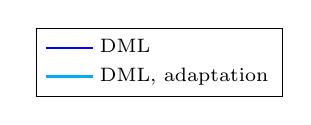
\begin{tikzpicture}[font=\scriptsize]

\begin{axis}[%
width=0.95092\figurewidth,
height=\figureheight,
at={(0\figurewidth,0\figureheight)},
scale only axis,
xmin=1,
xmax=50,
xlabel={Rank},
ymin=0,
ymax=1,
ylabel={Identification rate (\%)},
axis x line*=bottom,
axis y line*=left,
legend style={at={($ (0,1) + (+0.1cm,+0.1cm) $)},anchor=north west,align=left,legend cell align=left,draw=black},
xmajorgrids,
ymajorgrids,
grid style={dashed}
]
\addplot [color=blue,solid,line width=1.0pt]
  table[row sep=crcr]{%
1    0.1518987341772152\\
5    0.34810126582278483\\
10   0.47468354430379744\\
15   0.5474683544303798\\
20   0.5886075949367089\\
25   0.629746835443038\\
30   0.6613924050632911\\
35   0.680379746835443\\
40   0.7120253164556962\\
45   0.7183544303797469\\
50   0.7310126582278481\\
};
\addlegendentry{DML};

\addplot [color=cyan,solid,line width=1.0pt]
  table[row sep=crcr]{%
1    0.14556962025316456\\
5    0.3322784810126582\\
10   0.4873417721518987\\
15   0.5569620253164557\\
20   0.5917721518987342\\
25   0.6424050632911392\\
30   0.689873417721519\\
35   0.7025316455696202\\
40   0.7278481012658228\\
45   0.7531645569620253\\
50   0.7848101265822784\\
};
\addlegendentry{DML, adaptation};



\end{axis}
\end{tikzpicture}%
        \centering\small{(a) Whole CUHK02 $\rightarrow$ VIPeR}
        \label{fig:allcuhk_viper}
  
    &
        \setlength\figureheight{3.5cm}
        \setlength\figurewidth{3.5cm}
        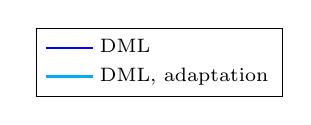
\begin{tikzpicture}[font=\scriptsize]

\begin{axis}[%
width=0.95092\figurewidth,
height=\figureheight,
at={(0\figurewidth,0\figureheight)},
scale only axis,
xmin=1,
xmax=50,
xlabel={Rank},
ymin=0,
ymax=1,
ylabel={Identification rate (\%)},
axis x line*=bottom,
axis y line*=left,
legend style={at={($ (0,1) + (+0.1cm,+0.1cm) $)},anchor=north west,align=left,legend cell align=left,draw=black},
xmajorgrids,
ymajorgrids,
grid style={dashed}
]
\addplot [color=blue,solid,line width=1.0pt]
  table[row sep=crcr]{%
1      0.126582278481 \\
5      0.303797468354 \\
10      0.414556962025 \\
15      0.490506329114 \\
20      0.550632911392 \\
25      0.613924050633 \\
30      0.651898734177 \\
35      0.686708860759 \\
40      0.708860759494 \\
45      0.75 \\
50      0.759493670886 \\
};
\addlegendentry{DML};

\addplot [color=cyan,solid,line width=1.0pt]
  table[row sep=crcr]{%
1      0.120253164557 \\
5      0.29746835443 \\
10      0.462025316456 \\
15      0.541139240506 \\
20      0.594936708861 \\
25      0.617088607595 \\
30      0.645569620253 \\
35      0.667721518987 \\
40      0.696202531646 \\
45      0.712025316456 \\
50      0.73417721519 \\
};
\addlegendentry{DML, adaptation};


\end{axis}
\end{tikzpicture}%
        \centering\small{(b) CUHK02/p1 $\rightarrow$ VIPeR}
%        \label{fig:CUHK02_p1_viper}
    &
        \setlength\figureheight{3.5cm}
        \setlength\figurewidth{3.5cm}
        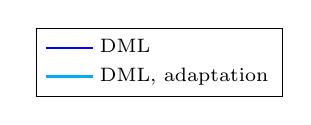
\begin{tikzpicture}[font=\scriptsize]

\begin{axis}[%
width=0.95092\figurewidth,
height=\figureheight,
at={(0\figurewidth,0\figureheight)},
scale only axis,
xmin=1,
xmax=50,
xlabel={Rank},
ymin=0,
ymax=1,
ylabel={Identification rate (\%)},
axis x line*=bottom,
axis y line*=left,
legend style={at={($ (0,1) + (+0.1cm,+0.1cm) $)},anchor=north west,align=left,legend cell align=left,draw=black},
xmajorgrids,
ymajorgrids,
grid style={dashed}
]
\addplot [color=blue,solid,line width=1.0pt]
  table[row sep=crcr]{%
1      0.0664556962025 \\
5      0.167721518987 \\
10      0.253164556962 \\
15      0.275316455696 \\
20      0.316455696203 \\
25      0.348101265823 \\
30      0.379746835443 \\
35      0.414556962025 \\
40      0.45253164557 \\
45      0.474683544304 \\
50      0.496835443038 \\
};
\addlegendentry{DML};

\addplot [color=cyan,solid,line width=1.0pt]
  table[row sep=crcr]{%
1      0.0632911392405 \\
5      0.161392405063 \\
10      0.259493670886 \\
15      0.338607594937 \\
20      0.389240506329 \\
25      0.417721518987 \\
30      0.439873417722 \\
35      0.471518987342 \\
40      0.496835443038 \\
45      0.518987341772 \\
50      0.53164556962 \\
};
\addlegendentry{DML, adaptation};


\end{axis}
\end{tikzpicture}%
        \centering\small{(c) PRID $\rightarrow$ VIPeR}
%        \label{fig:CUHK02_p1_viper} \\    
 \end{tabular}
%  \caption{Results on VIPeR}
%  \label{fig:viper}
% \end{figure}%

% \begin{figure}[h]
% \centering
 \begin{tabular}{ p{5cm}  p{5cm}  p{5cm} }
        \setlength\figureheight{3.5cm}
        \setlength\figurewidth{4cm}
        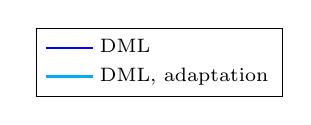
\begin{tikzpicture}[font=\scriptsize]

\begin{axis}[%
width=0.95092\figurewidth,
height=\figureheight,
at={(0\figurewidth,0\figureheight)},
scale only axis,
xmin=1,
xmax=50,
xlabel={Rank},
ymin=0,
ymax=1,
ylabel={Identification rate (\%)},
axis x line*=bottom,
axis y line*=left,
legend style={at={($ (0,1) + (+0.1cm,+0.1cm) $)},anchor=north west,align=left,legend cell align=left,draw=black},
xmajorgrids,
ymajorgrids,
grid style={dashed}
]
\addplot [color=blue,solid,line width=1.0pt]
  table[row sep=crcr]{%
1    0.08\\
5    0.13\\
10   0.22\\
15   0.27\\
20   0.31\\
25   0.35\\
30   0.4\\
35   0.41\\
40   0.41\\
45   0.43\\
50   0.44\\
};
\addlegendentry{DML};

\addplot [color=cyan,solid,line width=1.0pt]
  table[row sep=crcr]{%
1    0.07\\
5    0.19\\
10   0.27\\
15   0.32\\
20   0.35\\
25   0.37\\
30   0.39\\
35   0.41\\
40   0.43\\
45   0.45\\
50   0.45\\
};
\addlegendentry{DML, adaptation};


%[0.08, 0.13, 0.22, 0.27, 0.31, 0.35, 0.4, 0.41, 0.41, 0.43, 0.44]
%[0.07, 0.19, 0.27, 0.32, 0.35, 0.37, 0.39, 0.41, 0.43, 0.45, 0.45]

%
\end{axis}
\end{tikzpicture}%





        \centering\small{(d) Whole CUHK02 $\rightarrow$ PRID}
        \label{fig:allcuhk_prid}
    &
        \setlength\figureheight{3.5cm}
        \setlength\figurewidth{4cm}
        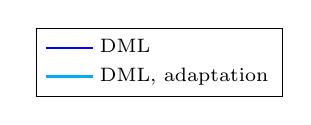
\begin{tikzpicture}[font=\scriptsize]

\begin{axis}[%
width=0.95092\figurewidth,
height=\figureheight,
at={(0\figurewidth,0\figureheight)},
scale only axis,
xmin=1,
xmax=50,
xlabel={Rank},
ymin=0,
ymax=1,
ylabel={Identification rate (\%)},
axis x line*=bottom,
axis y line*=left,
legend style={at={($ (0,1) + (+0.1cm,+0.1cm) $)},anchor=north west,align=left,legend cell align=left,draw=black},
xmajorgrids,
ymajorgrids,
grid style={dashed}
]
\addplot [color=blue,solid,line width=1.0pt]
  table[row sep=crcr]{%
1      0.04 \\
5      0.08 \\
10      0.15 \\
15      0.22 \\
20      0.25 \\
25      0.3 \\
30      0.32 \\
35      0.36 \\
40      0.39 \\
45      0.41 \\
50      0.44 \\
};
\addlegendentry{DML};

\addplot [color=cyan,solid,line width=1.0pt]
  table[row sep=crcr]{%
1      0.06 \\
5      0.16 \\
10      0.21 \\
15      0.27 \\
20      0.31 \\
25      0.36 \\
30      0.39 \\
35      0.41 \\
40      0.41 \\
45      0.42 \\
50      0.43 \\
};
\addlegendentry{DML, adaptation};


\end{axis}
\end{tikzpicture}%
        \centering\small{(e) CUHK02/p1 $\rightarrow$ PRID}
        \label{fig:CUHK02_p1_prid}
    &
       \setlength\figureheight{3.5cm}
       \setlength\figurewidth{4cm}
       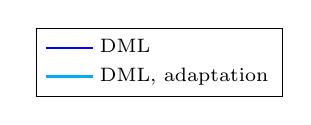
\begin{tikzpicture}[font=\scriptsize]

\begin{axis}[%
width=0.95092\figurewidth,
height=\figureheight,
at={(0\figurewidth,0\figureheight)},
scale only axis,
xmin=1,
xmax=50,
xlabel={Rank},
ymin=0,
ymax=1,
ylabel={Identification rate (\%)},
axis x line*=bottom,
axis y line*=left,
legend style={at={($ (0,1) + (+0.1cm,+0.1cm) $)},anchor=north west,align=left,legend cell align=left,draw=black},
xmajorgrids,
ymajorgrids,
grid style={dashed}
]
\addplot [color=blue,solid,line width=1.0pt]
  table[row sep=crcr]{%
1      0.08 \\
5      0.15 \\
10      0.19 \\
15      0.25 \\
20      0.28 \\
25      0.34 \\
30      0.35 \\
35      0.36 \\
40      0.39 \\
45      0.4 \\
50      0.41 \\
};
\addlegendentry{DML};

\addplot [color=cyan,solid,line width=1.0pt]
  table[row sep=crcr]{%
1      0.07 \\
5      0.19 \\
10      0.25 \\
15      0.27 \\
20      0.31 \\
25      0.36 \\
30      0.39 \\
35      0.42 \\
40      0.42 \\
45      0.46 \\
50      0.47 \\
};
\addlegendentry{DML, adaptation};


\end{axis}
\end{tikzpicture}%
        \centering\small{(f) VIPeR $\rightarrow$ PRID}
        \label{fig:viper_prid}  \\    
 \end{tabular}
%  \caption{Results on PRID}
%  \label{fig:prid}
% \end{figure}


% \begin{figure}[h]
% \centering
 \begin{tabular}{ p{5cm}  p{5cm}}
        \setlength\figureheight{3.5cm}
        \setlength\figurewidth{4cm}
        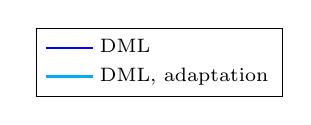
\begin{tikzpicture}[font=\scriptsize]

\begin{axis}[%
width=0.95092\figurewidth,
height=\figureheight,
at={(0\figurewidth,0\figureheight)},
scale only axis,
xmin=1,
xmax=50,
xlabel={Rank},
ymin=0,
ymax=1,
ylabel={Identification rate (\%)},
axis x line*=bottom,
axis y line*=left,
legend style={at={($ (0,1) + (+0.1cm,+0.1cm) $)},anchor=north west,align=left,legend cell align=left,draw=black},
xmajorgrids,
ymajorgrids,
grid style={dashed}
]
\addplot [color=blue,solid,line width=1.0pt]
  table[row sep=crcr]{%
1      0.109053497942 \\
5      0.265432098765 \\
10      0.366255144033 \\
15      0.407407407407 \\
20      0.465020576132 \\
25      0.491769547325 \\
30      0.510288065844 \\
35      0.541152263374 \\
40      0.572016460905 \\
45      0.59670781893 \\
50      0.617283950617 \\
};
\addlegendentry{DML};

\addplot [color=cyan,solid,line width=1.0pt]
  table[row sep=crcr]{%
1      0.125514403292 \\
5      0.253086419753 \\
10      0.366255144033 \\
15      0.440329218107 \\
20      0.5 \\
25      0.5329218107 \\
30      0.572016460905 \\
35      0.594650205761 \\
40      0.617283950617 \\
45      0.650205761317 \\
50      0.668724279835 \\
};
\addlegendentry{DML, adaptation};


\end{axis}
\end{tikzpicture}%
        \centering\small{(g) VIPeR $\rightarrow$ CUHK02/p1}
        \label{fig:viper_CUHK02_p1}
    &
        \setlength\figureheight{3.5cm}
        \setlength\figurewidth{4cm}
        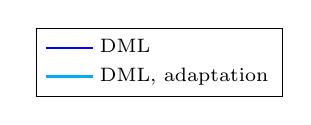
\begin{tikzpicture}[font=\scriptsize]

\begin{axis}[%
width=0.95092\figurewidth,
height=\figureheight,
at={(0\figurewidth,0\figureheight)},
scale only axis,
xmin=1,
xmax=50,
xlabel={Rank},
ymin=0,
ymax=1,
ylabel={Identification rate (\%)},
axis x line*=bottom,
axis y line*=left,
legend style={at={($ (0,1) + (+0.1cm,+0.1cm) $)},anchor=north west,align=left,legend cell align=left,draw=black},
xmajorgrids,
ymajorgrids,
grid style={dashed}
]
\addplot [color=blue,solid,line width=1.0pt]
  table[row sep=crcr]{%
1      0.0569620253165 \\
5      0.139240506329 \\
10      0.212025316456 \\
15      0.284810126582 \\
20      0.316455696203 \\
25      0.344936708861 \\
30      0.370253164557 \\
35      0.389240506329 \\
40      0.414556962025 \\
45      0.443037974684 \\
50      0.465189873418 \\
};
\addlegendentry{DML};

\addplot [color=cyan,solid,line width=1.0pt]
  table[row sep=crcr]{%
1      0.0843621399177 \\
5      0.191358024691 \\
10      0.263374485597 \\
15      0.316872427984 \\
20      0.347736625514 \\
25      0.395061728395 \\
30      0.432098765432 \\
35      0.471193415638 \\
40      0.504115226337 \\
45      0.5329218107 \\
50      0.553497942387 \\
};
\addlegendentry{DML, adaptation};


\end{axis}
\end{tikzpicture}%
        \centering\small{(h) PRID $\rightarrow$ CUHK02/p1}
        \label{fig:prid_CUHK02_p1}
  \\    
  \end{tabular}
  \caption{Results on VIPeR, PRID and CUHK02/p1 with and without domain-adversarial learning. Across the eight domain pairs domain-adversarial learning improves re-identification accuracy. For some domain pairs the improvement is considerable.}
  \label{fig:adaptresults}
\end{figure}

Figure \ref{fig:adaptresults} shows results in the form of Rekall@K metric for eight pairs of datasets. Depending on the hardness of the annotation problem we trained either for 50,000 iterations (CUHK02/p1 $\rightarrow$ VIPeR, VIPeR $\rightarrow$ CUHK02/p1, PRID $\rightarrow$ VIPeR) or for 20,000 iterations (the other five pairs). 

\begin{figure*}
\centering
\begin{tabular}{c c}
\includegraphics[height=7cm, width=7cm]{Chapters/gradrev/figures/reid_adapt_results/viper_cuhkp1_zc.png}&
\includegraphics[height=7cm, width=7cm]{Chapters/gradrev/figures/reid_adapt_results/viper_cuhkp1_da.png}\\
\small{(a) DML}&
\small{(b) DML, adaptation}\\
\end{tabular}
\caption{The effect of adaptation shown by t-SNE visualizations of source and target domains descriptors in a VIPeR $\rightarrow$ CUHK02/p1 experiment pair. VIPeR is depicted with \textit{green} and CUHK02/p1 - with \textit{red}. As in the image classification case, domain-adversarial learning ensures a closer match between the source and the target distributions. }
\label{fig:reidtsne}
\end{figure*}


After the sufficient number of iterations, domain-adversarial training consistently improves the performance of re-identification. For the pairs that involve PRID dataset, which is more dissimilar to the other two datasets, the improvement is considerable. Overall, this demonstrates the applicability of the domain-adversarial learning beyond classification problems.

Figure \ref{fig:reidtsne} further demonstrates the effect of adaptation on the distributions of the learned descriptors in the source and in target sets in VIPeR $\rightarrow$ CUHK02/p1 experiments, where domain adversarial learning once again achieves better intermixing of the two domains.


\section{Conclusion}

The chapter describes a new approach to domain adaptation of feed-forward neural networks, which allows large-scale training based on large amount of annotated data in the source domain and large amount of unannotated data in the target domain. Similarly to many previous shallow and deep DA techniques, the adaptation is achieved through aligning the distributions of features across the two domains. However, unlike previous approaches, the alignment is accomplished through standard backpropagation training.

%The approach is motivated and supported by the domain adaptation theory of \citet{BenDavid-NIPS06}. 
 The main idea behind DANN is to enjoin the network hidden layer to learn a representation which is predictive of the source example labels, but uninformative about the domain of the input (source or target). 
% We implement this new approach within both shallow and deep feed-forward architectures. The latter allows simple implementation within virtually any deep learning package through the introduction of a simple gradient reversal layer. 
%We have shown that our approach is flexible and improves the results for classification tasks as well as person re-identification. 

A convenient aspect of our approach is that the domain adaptation component can be added to almost any neural network architecture that is trainable with backpropagation. Towards this end, we have demonstrated experimentally that the approach is not confined to classification tasks but can be used in other feed-forward architectures, e.g.\ for descriptor learning for person re-identification. The full set of experiments, including those for classification, is presented in the corresponding publication \citep{ganin2016domain}.

% Further evaluation on larger-scale tasks and in semi-supervised settings constitutes future work. It is also interesting whether the approach can benefit from a good initialization of the feature extractor. For this, a natural choice would be to use deep autoencoder/deconvolution network trained on both domains (or on the target domain) in the same vein as \citet{Glorot11,Chopra13}, effectively using \citet{Glorot11,Chopra13} as an initialization to our method.

%\pagebreak

% \acks{This work has been supported by National Science and Engineering Research Council (NSERC) Discovery
% grants 262067 and 0122405 as well as the Russian Ministry of Science and Education grant RFMEFI57914X0071.
% Computations were performed on the Colosse supercomputer grid at Universit\'e Laval, under the auspices of Calcul Qu\'ebec and Compute Canada. The operations of Colosse are funded by the NSERC, the Canada Foundation for Innovation (CFI), NanoQu\'ebec, and the Fonds de recherche du Qu\'ebec -- Nature et technologies (FRQNT). We also thank the Graphics \& Media Lab, Faculty of Computational Mathematics and Cybernetics, Lomonosov Moscow State University for providing the synthetic road signs dataset.}


% \iffalse

% \appendix

% \section{Shallow DANN Algorithm}
% \label{supmat:shallow_DANN}

% In the pseudocode of Algorithm~\ref{alg:stoch-up}, we use
% $\ee(y)$ to refer to a ``one-hot'' vector, consisting of all $0$s except for a $1$ at position~$y$. Also, $\odot$ is the element-wise product.
% %Notice that, on Line~\ref{algoline:da} of Algorithm~\ref{alg:stoch-up}, the....

% \iffalse
% To optimize Equation~\eqref{eqn:global}, one option would be to follow a hard-EM approach,
% where we would alternate between optimizing until convergence the adversarial parameters $\uu, d$ and the
% other regular neural network parameters $\WW, \VV, \bb, \cc$. However, we've found that a simpler stochastic gradient approach is sufficient and works well in practice. Here, the stochastic gradient approach consists in sampling a pair of source and target example $\xb_i, \xb_j$ and updating a gradient step update of all parameters of DANN. Crucially, while the update of the regular parameters follows as usual the opposite direction of the gradient, for the adversarial parameters $\uu, d$ the step must follow the gradient's direction (since we maximize with respect to them, instead of minimizing). 
% \fi 

% %\afterpage{
% \begin{algorithm}[t]
%   \caption{Shallow DANN -- Stochastic training update}
%   \label{alg:stoch-up}
% %   \algsetup{
% %   linenosize=\small,
% %   linenodelimiter=.
% %   }
% \begin{multicols}{2}
% \begin{algorithmic}[1]
% {\footnotesize
%   \STATE {\bfseries Input:} \\
%   --- samples $S=\{(\xb_i, \ys_i)\}_{i=1}^n$ and $T=\{\xb_i\}_{i=1}^{n'}$,\\
%   --- hidden layer size $D$, \\
%   --- adaptation parameter $\lambda$,\\
%   --- learning rate $\mu$,
%   \STATE {\bfseries Output:} neural network $\{\WW, \VV, \bb, \cc\}$ 
%   \vspace{2mm}
% %   \STATE 
%   \STATE $\WW, \VV \leftarrow {\rm random\_init}(\,D\,)$
%   \STATE $\bb, \cc, \uu, d \leftarrow 0$
%   \WHILE{stopping criteria is not met}
%   \FOR{$i$ from 1 to $n$}
%   \STATE \# {\tt Forward propagation}
%   \STATE $G_f(\xb_i) \leftarrow \sigm(\bb + \WW\xb_i)$
%   \STATE $G_y(G_f(\xb_i)) \leftarrow \softmax(\cc + \VV G_f(\xb_i))$
%   \vspace{1.5mm}
%   \STATE \# {\tt Backpropagation}
%   \STATE $\Delta_{\cc} \leftarrow -(\ee(\ys_i)-G_y(G_f(\xb_i)))$ 
%   % \# $\ee(y)$ is a ``one-hot'' vector, that is all 0s but with a 1 at position~$y$
%   \STATE $\Delta_{\VV} \leftarrow \Delta_{\cc}~G_f(\xb_i)^\top$ 
%   \STATE $\Delta_{\bb} \leftarrow \left(\VV^{\top} \Delta_{\cc}\right) \odot G_f(\xb_i) \odot (1-G_f(\xb_i))$
%   % \# $\odot$ is the element-wise product
%   \STATE $\Delta_{\WW} \leftarrow \Delta_{\bb} \cdot({\xb_i})^\top$
%   \vspace{1.5mm}
%   \STATE \# {\tt Domain adaptation regularizer...}
%   \STATE \# {\tt ...from current domain}
%   \STATE $G_d(G_f(\xb_i)) \leftarrow \sigm(d + \uu^\top G_f(\xb_i))$
%   \STATE $\Delta_d \leftarrow \lambda (1-G_d(G_f(\xb_i)))$ 
%   \STATE $\Delta_{\uu} \leftarrow \lambda(1-G_d(G_f(\xb_i))) G_f(\xb_i)$
%   \STATE ${\rm tmp} \leftarrow \lambda(1-G_d(G_f(\xb_i)))$\\*
%   ~~~~~~~~~~~~~~~${}\times\uu \odot G_f(\xb_i) \odot (1-G_f(\xb_i))$
%   \STATE $\Delta_{\bb} \leftarrow \Delta_{\bb} + {\rm tmp}$ 
%   \STATE $\Delta_{\WW} \leftarrow \Delta_{\WW} + {\rm tmp}\cdot({\xb_i})^\top$
%   \label{algoline:omit1}
%       \vspace{1.5mm}
%   \STATE \# {\tt ...from other domain}
%   \STATE $j \leftarrow {\rm uniform\_integer}(1,\dots,n')$
%   \STATE $G_f(\xb_j) \leftarrow \sigm(\bb + \WW\xb_j)$
%   \STATE $G_d(G_f(\xb_j)) \leftarrow \sigm(d + \uu^\top G_f(\xb_j))$ 
%   \STATE $\Delta_d \leftarrow \Delta_d - \lambda G_d(G_f(\xb_j))$
%   \STATE $\Delta_{\uu} \leftarrow \Delta_{\uu} - \lambda G_d(G_f(\xb_j)) G_f(\xb_j)$
%   \STATE ${\rm tmp} \leftarrow -\lambda G_d(G_f(\xb_j))$\\*
%   ~~~~~~~~~~~~~~~${}\times\uu \odot G_f(\xb_j) \odot (1-G_f(\xb_j))$
%   \STATE $\Delta_{\bb} \leftarrow \Delta_{\bb} + {\rm tmp}$ 
%   \STATE $\Delta_{\WW} \leftarrow \Delta_{\WW} + {\rm tmp}\cdot(\xb_j)^\top$
%   \label{algoline:omit2}
%       \vspace{1.5mm}
%   \STATE \# {\tt Update neural network parameters}
%   \STATE $\WW \leftarrow \WW - \mu \Delta_{\WW}$ 
%   \STATE $\VV \leftarrow \VV - \mu \Delta_{\VV}$
%   \STATE $\bb \leftarrow \bb - \mu \Delta_{\bb}$ 
%   \STATE $\cc \leftarrow \cc - \mu \Delta_{\cc}$
%       \vspace{1.5mm}
%   \STATE \# {\tt Update domain classifier}
% %   \STATE $\uu \leftarrow \uu + \mu \Delta_{\uu}$ \# Notice the ``+'' instead of the ``-''
% %   \STATE $d \leftarrow d + \mu \Delta_{d}$
%   \STATE $\uu \leftarrow \uu + \mu \Delta_{\uu}$ 
%   \STATE $d \leftarrow d + \mu \Delta_{d}$
%   \label{algoline:da}
%       \ENDFOR
%   \ENDWHILE
% %   \STATE 
% %   \RETURN $\{\WW, \VV, \bb, \cc\}$
%   } 
% \end{algorithmic}
% \end{multicols}
% \end{algorithm}
% %}

% \medskip


% \iffalse
% \section{An alternative optimization approach}
% \label{supmat:alternative_optimization}


% \def\x{{\mathbf x}}
% \def\f{{\mathbf f}}

% \def\S{{\cal S}}
% \def\T{{\cal T}}

% \def\R{{\mathds R}}

% \def\tf{{\theta_f}}
% \def\td{{\theta_d}}
% \def\ty{{\theta_y}}
% \def\htf{{\hat\theta_f}}
% \def\htd{{\hat\theta_d}}
% \def\hty{{\hat\theta_y}}

% There exists an alternative construction \citep[inspired by][]{Goodfellow14} that leads to the same updates \eq{upd1}-\eq{upd3}. Rather than using the gradient reversal layer, the construction introduces two different loss functions for the domain classifier. Minimization of the first domain loss ($ L_{d+} $) should lead to a better domain discrimination, while the second domain loss ($ L_{d-} $) is minimized when the domains are distinct. Stochastic updates for $ \theta_f $ and $ \theta_d $ are then defined as:
% \begin{align*}
%   \tf \quad &\longleftarrow \quad \tf \;-\; \mu \left(\frac{\partial \Lcal_y^i}{\partial \tf} + \frac{\partial \Lcal^i_{d-}}{\partial \tf} \right)\\
%   \td \quad &\longleftarrow \qquad \td \;-\; \mu \frac{\partial \Lcal^i_{d+}}{\partial \td} \, ,
% \end{align*}
% Thus, different parameters participate in the optimization of different losses

% In this framework, the gradient reversal layer constitutes a special case, corresponding  to the pair of domain losses $ (\Lcal_d, -\lambda \,\Lcal_d) $. However, other pairs of loss functions can be used. One example would be the binomial cross-entropy \citep{Goodfellow14}:
% \begin{equation*}
%   \Lcal_{d+}(q, d) = \sum_{i = 1..N} d_i \log(q_i) + (1 - d_i) \log(1 - q_i) \, ,
% \end{equation*}
% where $ d $ indicates domain indices and $ q $ is an output of the predictor. In that case ``adversarial'' loss is easily obtained by swapping domain labels, \ie, $ L_{d-}(q, d) = L_{d+}(q, 1 - d) $. This particular pair has a potential advantage of producing stronger gradients at early learning stages if the domains are quite dissimilar. In our experiments, however, we did not observe any significant improvement resulting from this choice of losses.
% \fi

% \iffalse
% \section{CNN architectures}
% \label{supmat:CNN}

% \begin{figure*}[t]
%   \definecolor{fnodebottom}{RGB}{132,170,81}
%   \definecolor{fnodetop}{RGB}{172,222,106}
%   \definecolor{cnodebottom}{RGB}{120,128,164}
%   \definecolor{cnodetop}{RGB}{158,167,218}
%   \definecolor{dnodebottom}{RGB}{174,109,146}
%   \definecolor{dnodetop}{RGB}{230,141,192}
%   \centering
%   \subfloat[MNIST architecture]{%
%     \scalebox{0.65}{\begin{tikzpicture}[
  black!50, text=black,
  node distance=4mm,
  grlnode/.style={
    align=center,
    circle,minimum size=6mm,
    inner sep=5pt,
    very thick,draw=black!50,
    font=\ttfamily
  },
  fnode/.style={
    align=center,
    % The shape:
    rectangle,minimum size=6mm,rounded corners,
    % The rest
    inner sep=5pt,
    very thick,draw=black!50,
    top color=fnodetop,bottom color=fnodebottom,
    font=\ttfamily},
  cnode/.style={
    fnode,top color=cnodetop,bottom color=cnodebottom},
  dnode/.style={
    fnode,top color=dnodetop,bottom color=dnodebottom},
  vhedge/.style={
    rounded corners,to path=|- (\tikztotarget)}]
  \matrix[row sep=5mm,column sep=5mm] {
    \node (conv1) [fnode] {conv 5x5\\32 maps\\ReLU}; &
    \node (pool1) [fnode] {max-pool 2x2\\2x2 stride}; &
    \node (conv2) [fnode] {conv 5x5\\48 maps\\ReLU}; &
    \node (pool2) [fnode] {max-pool 2x2\\2x2 stride}; &
  
    \node (fc3)   [cnode] {fully-conn\\100 units\\ReLU}; &
    \node (fc4)   [cnode] {fully-conn\\100 units\\ReLU}; &
    \node (fc5)   [cnode] {fully-conn\\10 units\\Soft-max}; \\
  
    & & &
    \node (grl) [grlnode] {GRL}; &
  
    \node (fc1_d) [dnode] {fully-conn\\100 units\\ReLU}; &
    \node (fc2_d) [dnode] {fully-conn\\1 unit\\Logistic}; \\
  };
  
  \path (conv1) edge[-latex,shorten >=1pt,very thick] (pool1);
  \path (pool1) edge[-latex,shorten >=1pt,very thick] (conv2);
  \path (conv2) edge[-latex,shorten >=1pt,very thick] (pool2);
  \path (pool2) edge[-latex,shorten >=1pt,very thick] (fc3);
  \path (fc3)   edge[-latex,shorten >=1pt,very thick] (fc4);
  \path (fc4)   edge[-latex,shorten >=1pt,very thick] (fc5);
  
  \path (pool2.south) edge[-latex,shorten >=1pt,very thick] (grl.north);
  \path (grl) edge[-latex,shorten >=1pt,very thick] (fc1_d);
  \path (fc1_d) edge[-latex,shorten >=1pt,very thick] (fc2_d);
\end{tikzpicture}
}}\\
%   \subfloat[SVHN architecture]{%
%     \scalebox{0.65}{\begin{tikzpicture}[
  black!50, text=black,
  node distance=4mm,
  grlnode/.style={
    align=center,
    circle,minimum size=6mm,
    inner sep=5pt,
    very thick,draw=black!50,
    font=\ttfamily
  },
  fnode/.style={
    align=center,
    % The shape:
    rectangle,minimum size=6mm,rounded corners,
    % The rest
    inner sep=5pt,
    very thick,draw=black!50,
    top color=fnodetop,bottom color=fnodebottom,
    font=\ttfamily},
  cnode/.style={
    fnode,top color=cnodetop,bottom color=cnodebottom},
  dnode/.style={
    fnode,top color=dnodetop,bottom color=dnodebottom},
  vhedge/.style={
    rounded corners,to path=|- (\tikztotarget)}]
  \matrix[row sep=5mm,column sep=5mm] {
    \node (conv1) [fnode] {conv 5x5\\64 maps\\ReLU}; &
    \node (pool1) [fnode] {max-pool 3x3\\2x2 stride}; &
    \node (conv2) [fnode] {conv 5x5\\64 maps\\ReLU}; &
    \node (pool2) [fnode] {max-pool 3x3\\2x2 stride}; &
    \node (conv3) [fnode] {conv 5x5\\128 maps\\ReLU}; &
  
    \node (fc4)   [cnode] {fully-conn\\3072 units\\ReLU}; &
    \node (fc5)   [cnode] {fully-conn\\2048 units\\ReLU}; &
    \node (fc6)   [cnode] {fully-conn\\10 units\\Soft-max}; \\
  
    & & & &
    \node (grl) [grlnode] {GRL}; &
    \node (fc1_d) [dnode] {fully-conn\\1024 units\\ReLU}; &
    \node (fc2_d) [dnode] {fully-conn\\1024 units\\ReLU}; &
    \node (fc3_d) [dnode] {fully-conn\\1 unit\\Logistic}; \\
  };
  
  \path (conv1) edge[-latex,shorten >=1pt,very thick] (pool1);
  \path (pool1) edge[-latex,shorten >=1pt,very thick] (conv2);
  \path (conv2) edge[-latex,shorten >=1pt,very thick] (pool2);
  \path (pool2) edge[-latex,shorten >=1pt,very thick] (conv3);
  \path (conv3) edge[-latex,shorten >=1pt,very thick] (fc4);
  \path (fc4)   edge[-latex,shorten >=1pt,very thick] (fc5);
  \path (fc5)   edge[-latex,shorten >=1pt,very thick] (fc6);
  
  \path (conv3.south) edge[-latex,shorten >=1pt,very thick] (grl.north);
  \path (grl) edge[-latex,shorten >=1pt,very thick] (fc1_d);
  \path (fc1_d) edge[-latex,shorten >=1pt,very thick] (fc2_d);
  \path (fc2_d) edge[-latex,shorten >=1pt,very thick] (fc3_d);
\end{tikzpicture}
}}\\
%   \subfloat[GTSRB architecture]{%
%     \scalebox{0.55}{\begin{tikzpicture}[
  black!50, text=black,
  node distance=4mm,
  grlnode/.style={
    align=center,
    circle,minimum size=6mm,
    inner sep=5pt,
    very thick,draw=black!50,
    font=\ttfamily
  },
  fnode/.style={
    align=center,
    % The shape:
    rectangle,minimum size=6mm,rounded corners,
    % The rest
    inner sep=5pt,
    very thick,draw=black!50,
    top color=fnodetop,bottom color=fnodebottom,
    font=\ttfamily},
  cnode/.style={
    fnode,top color=cnodetop,bottom color=cnodebottom},
  dnode/.style={
    fnode,top color=dnodetop,bottom color=dnodebottom},
  vhedge/.style={
    rounded corners,to path=|- (\tikztotarget)}]
  \matrix[row sep=5mm,column sep=5mm] {
    \node (conv1) [fnode] {conv 5x5\\96 maps\\ReLU}; &
    \node (pool1) [fnode] {max-pool 2x2\\2x2 stride}; &
    \node (conv2) [fnode] {conv 3x3\\144 maps\\ReLU}; &
    \node (pool2) [fnode] {max-pool 2x2\\2x2 stride}; &
    \node (conv3) [fnode] {conv 5x5\\256 maps\\ReLU}; &
    \node (pool3) [fnode] {max-pool 2x2\\2x2 stride}; &
  
    \node (fc4)   [cnode] {fully-conn\\512 units\\ReLU}; &
    \node (fc5)   [cnode] {fully-conn\\10 units\\Soft-max}; \\
  
    & & & & &
    \node (grl) [grlnode] {GRL}; &
    \node (fc1_d) [dnode] {fully-conn\\1024 units\\ReLU}; &
    \node (fc2_d) [dnode] {fully-conn\\1024 units\\ReLU}; &
    \node (fc3_d) [dnode] {fully-conn\\1 unit\\Logistic}; \\
  };
  
  \path (conv1) edge[-latex,shorten >=1pt,very thick] (pool1);
  \path (pool1) edge[-latex,shorten >=1pt,very thick] (conv2);
  \path (conv2) edge[-latex,shorten >=1pt,very thick] (pool2);
  \path (pool2) edge[-latex,shorten >=1pt,very thick] (conv3);
  \path (conv3) edge[-latex,shorten >=1pt,very thick] (pool3);
  \path (pool3) edge[-latex,shorten >=1pt,very thick] (fc4);
  \path (fc4)   edge[-latex,shorten >=1pt,very thick] (fc5);
  
  \path (pool3.south) edge[-latex,shorten >=1pt,very thick] (grl.north);
  \path (grl) edge[-latex,shorten >=1pt,very thick] (fc1_d);
  \path (fc1_d) edge[-latex,shorten >=1pt,very thick] (fc2_d);
  \path (fc2_d) edge[-latex,shorten >=1pt,very thick] (fc3_d);
\end{tikzpicture}
}}\\
% %   \subfloat[CIFAR-10 architecture]{%
% %     \scalebox{0.65}{\input{Chapters/gradrev/archs/cifar10.tikz}}}
%   \caption{CNN architectures used in the experiments. Boxes correspond to transformations applied to the data. Color-coding is the same as in \fig{arch}.}
%   \label{fig:exper_archs}
% \end{figure*}

% Four different architectures were used in our experiments (first three are shown in \fig{exper_archs}):
% \begin{itemize}
%   \item A smaller one (a) if the source domain is MNIST. This architecture was inspired by the classical LeNet-5 \citep{LeCun98}.
%   \item (b) for the experiments involving SVHN dataset. This one is adopted from \citet{Srivastava14}.
%   \item (c) in the {\sc Syn Sings} $ \rightarrow $ {\sc GTSRB} setting. We used the single-CNN baseline from \citet{Cirecsan12} as our starting point.
%   \item Finally, we use pre-trained \texttt{AlexNet} from the \texttt{Caffe}-package \citep{Jia14} for the {\sc Office} domains. Adaptation architecture is identical to \citet{Tzeng14}: 2-layer domain classifier ($x\rightarrow1024\rightarrow1024\rightarrow2$) is attached to the $ 256 $-dimensional bottleneck of \texttt{fc7}.  
% \end{itemize}
% The domain classifier branch in all cases is somewhat arbitrary (better adaptation performance might be attained if this part of the architecture is tuned).

% \section{Training procedure}
% \label{supmat:traning_procedure}

% We use stochastic gradient descent with 0.9 momentum and the learning rate annealing described by the following formula:
% \begin{equation*}
%   \mu_p = \frac{\mu_0}{(1 + \alpha \cdot p)^\beta} \, , 
% \end{equation*}
% where $ p $ is the training progress linearly changing from 0 to 1, $ \mu_0 = 0.01 $, $ \alpha = 10 $ and $ \beta = 0.75 $ (the schedule was optimized to promote convergence and low error on the \emph{source} domain).

% Following \citet{Srivastava14} we also use dropout and $ \ell_2 $-norm restriction when we train the SVHN architecture.
% \fi


% \newpage 
% 
%\newcommand{\root}{Chapters/facev1}

\chapter{Getting Off the Internet: Practical Domain Adaptation for Face Recognition}
\label{chapt:wildface}


\section{Motivation}
%face
For face recognition, one important cross-domain scenario is related to using powerful models pretrained on professional photographs for surveillance data. As it has been already mentioned in \sect{face}, large-scale training datasets for face recognition most often include high-quality images that are very different from those captured by surveillance systems. In person re-identification, the domain difference comes mainly from the illumination condition variations between the camera sets (if the difference of the camera positions is put aside). In contrast,  surveillance face recognition implies a complex domain shift caused by a combination of low resolution, compression and illumination conditions. 


In particular, in this chapter we study the unsupervised domain adaptation scenario, where face recognition is trained using an annotated Internet face dataset and an unannotated dataset of faces collected from a surveillance camera network with low image quality. We mostly focus on the recent class of methods that consider domain-adaptation at the image level. We thus investigate how image transformation achieved with recent unsupervised image transformation techniques such as CycleGAN \citep{ZhuPIE17} can be used for face recognition under strong domain shifts. 

We compare and evaluate several strategies, such as transferring test data to the Internet image domain,  transferring training data to the target domain followed by retraining the network. As a baseline, we also compare to adversarial domain adaptation at feature level described in \chapt{gradrev}.% \cite{GaninUAGLLML16}. 

Our comparison suggests that image transformation (without explicit modeling of separate degradation factors) can be used for unsupervised domain adaptation of face recognition. We, however, demonstrate that special care needs to be taken in order to make such domain adaptation work better than baselines, and come up with practical suggestions on how such improvement can be achieved.

%model
% Since the CycleGAN \cite{cyclegan} architecture for image-to-image translation and stylization appeared, domain adaptation has become one of its active fields of application. This approach differs from the feature-level domain adaptation techniques of \cite{LongC0J15} and \cite{tzeng2014deep} or the method presented in the \chapt{gradrev}, because rather than finding deep domain-invariant representations, it works on the pixel level and aims at building mappings between the image domains. Thus the domain adaptation is done in two steps: building a mapping the source domain to target and retraining the predictor on the transferred source data. (Although it is also possible to combine these two steps into one optimization process.)%cycada

% %pedestrians
% For person re-identification, the pixel-level domain adaptation with CycleGAN has been applied in several recent works \cite{} (after the results of the \chapt{gradrev} were published). Some of them consider different datasets as domains, others aim at utilising synthetic re-identification data to improve the results on real data \cite{}. As demonstrated by these works, image-to-image translation may help a lot to overcome the illumination differences between the source and target camera sets. %Still, to the best of our knowledge, there are no works approaching face recognition for surveillance data.

% This chapter demonstrates the performance of the pixel-level domain adaptation approach based on CycleGAN model in the presence of an extreme domain shift between the usual face recognition training data and surveillance data. The considered surveillance data are harvested from $6$ surveillance cameras in the Moscow subway. Two publicly available face recognition datasets of different image quality are considered for the source domain. The approach is compared to several important baselines, including the reverse translation of the target images back to the source domain and the feature-level domain adaptation suggested in this chapter.

%The remainder of the chapter is organized as follows. Image-level domain transfer and face recognition methods are described in \sect{method}.  We define the variants of the training data augmentation compared in this work in \sect{ft}. Then we give the implementation details in \sect{training}. The quantitative comparisons of the described methods and baselines are presented in \sect{results}. Finally, we conclude the work with discussion and summary in \sect{conclusion}.



%\titlerunning{Short form of title}        % if too long for running head



% \begin{abstract}
% Face recognition in real surveillance scenarios is challenging due to the presence of complex degradation factors. At the same time, the easiest-to-collect and the biggest available training data for face recognition come from the Internet, where images and video frames have higher quality, higher resolution, and better lighting. In this work, we study training face recognition systems under such domain shift. We show that CycleGAN technique can be utilized for transferring labeled training data into the target domain of surveillance camera, and that the transferred data can be used to train face recognition in the new domain. We compare this approach to several baselines including the domain transfer in the opposite direction to turn test data directly to the high-quality domain. Our comparison and evaluation allow us to come up with a viable strategy for training face recognition in surveillance data.
% \keywords{face recognition \and surveillance \and domain adaptation}
% % \PACS{PACS code1 \and PACS code2 \and more}
% % \subclass{MSC code1 \and MSC code2 \and more}
% \end{abstract}


%% !TEX root = ../Thesis_main.tex
\chapter{Introduction}

%video surveillance+
%person re-id+
% originates from Multi-Target Multi-Camera Tracking 
%open world / closed world+
%face : verification/identification
%common aspects: detection , processing, recognition
%deep learning

%retrieval
%fine-grained recognition
%adaptation

%datasets (cut from the papers) + table with reid dataset?
%architectures
%definitions?
%contribution - what is done
\section{Context}
\subsection{Problem of 3D reconstruction}

\subsection{Approaches for solving 3D Reconstruction problem}

Solutions for a reconstruction problem can be grouped in two major groups: 1) Geometric approach - when problem is represented as optimisation of scene state given constrains on projections of scene state to data, 2) Machine Learning approach - inverse model is optimisation.

If $X$ - is scene data, $z$ - is the state of the scene, and $g_i(z)$ - projection function of 3D scene $z$ state to perspective $i$, then to find an optimal 3D reconstruction, one solves this minimisation problem:
\begin{equation}
z_{rec} = \min_z\sum_i|X_i-g_i(z)|_2 .
\end{equation}

This approach only solves problem for once scene and does not provide any semantic information about it, only basic geometric information. 
The second approach is more modern and better fitted for machine learning applications, because instead of optimizing state of the scene, it's optimizes a model that performs computation from input data to some semantic (intrinsic) parameters, and can be described as following optimisation procedure:
\begin{equation}
\min_\theta\sum_i|X_i-g_i(f_\theta(\pi))|_2,\ \ \pi=I_\theta(\{X_i\}_i),\ \ z=f_\theta(\pi),
\end{equation}
where $\pi$ - are scene parameters, $f_\theta(\pi)$ - is a generative model that generates 3D state $z$ and it's function is determined by tunable parameters $\theta$.

In reconstruction process information can be introduced in two possible ways: 1) input signal - data measured by some spatial sensor, 2) by adding a priori knowledge while training the Inverse model or by design choice of reconstruction algprithm. Between the two source exist a fundamental trade-off and detirmination of which is dominant can be quite difficult \cite{tatarchenko2019single}.


\subsection{Objectives and Motivations}

The goal of this work to improve methods of 3D reconstruction in holistic context using deep learning systems. For efficient applications such as robotics in human environments and mixed reality more advanced machine perception systems are needed. Human perception is a complex system with several properties not all of which are replicated in modern machine perception systems. From cognitive sciences it's known that ability to model environments is one of the most important for perception system, in area of computer vision this is known as an ability to perform \textit{3D reconstruction} of scenes and environments. To solve this problem in a general case requires application of machine learning.

In particular, the development of such holistic deep 3D reconstruction system includes several important tasks:

\begin{itemize}
􏰀    \item Capturing scenes, complete with colour and depth data of a sufficient quality,
    \item Recalling objects from large scale database of objects,
    \item Segmenting variety of most common elements from sensor data, such as household objects and architectural components,
    \item Detecting and reconstructing shape and pose of and human bodies.
\end{itemize}

Each of these sub-tasks constitutes a challenge in the context of human perception.

The presence of noise in sensor data (e.g., consumer grade depth cameras) is a serious problem for all downstream sub-tasks, low fidelity of this data causes a considerable compaunding performance drop.

\subsection{3D data representations}

We can describe a 3D object in multiple ways, and codification of it's properties has ramifications about capturing different information about objects and scenes, as well as kinds of models that can regenerate them or computational resources needed to process it.
Each representation has it's own pros and cons. We assume 3D information representation to be positive effective and usefull if it captures more relevant information with less storage requirement (compression), increases signal to noise ratio of data, captures shape and texture properties with minimum trade-off.

Here are some popular examples of 3D data representations:
\begin{enumerate}
	\item Multiple 2D projections - captures surface texture, highly redundant representation if images overlap, also vulnerable to optic illusions.
	\item Voxels - simple, most of the time can be sparse, represents rough volumetric properties vell but losses most of surface properties.
	\item Point Cloud - are sparse in a sense that they don't capture empty space, losing all surface properties besides color and estimated normals and most of volumetric properties.
	\item 2.5D (RGB-D) images are widespread because of cheap measurement devices, capture volumentric depth but succeptable to occlusion of bodies in a scene and records a lot of noise with actual signal.
\end{enumerate}



%Motivation: RGB-D scanning is here and we want to have a fine-grained understanding of the 3D captures
In the recent years, a wide variety of consumer-grade RGB-D sensors, such as the Intel Real Sense, Microsoft Kinect, depth-sensor enabled smartphones, enabled inexpensive and rapid RGB-D data acquisition. Increasing availability of large, labeled datasets (e.g.,~\cite{chang2017matterport3d,dai2017scannet})  made possible development of deep learning methods for 3D object classification and semantic segmentation. At the same time, acquired 3D data is often incomplete and noisy; while one can identify and segment the objects in the scene, reconstructing high-quality geometry of objects remains a challenging problem.  

An example of the new approach in recent work 
\cite{avetisyan2019scan2cad}, uses a large dataset of clean, labeled geometric shapes
\cite{chang2015shapenet}, for classification/segmentation associating the input point or voxel data with object labels from the dataset, along with adapting geometry to 3D data.  This approach ensures that the output geometry has high quality, and is robust with respect to noise and missing data in the input.  
At the same time, a ``flat'' classification/segmentation approach, with each object in the database corresponding to a separate label and matched to a subpart of the input data corresponding to the whole object, does not scale well as the number of classes grows and often runs into difficulties in the cases of extreme occlusion (only a relatively small part of an object is visible). 
Significant improvements can be achieved by considering object \emph{parts}, or more generally part hierarchies. 
Part-based segmentation of 3D datasets promises to offer a significant improvement both in finding the best matching shape in the dataset, recognizing objects from  highly incomplete data (e.g., from a couple of parts) from  as well as more precise geometry adaptation as well as, potentially, assembly of new shapes out of existing parts yielding a closer match to the input data. 

large collection of 3D models in database can be reduced to structured representations, 
objects with occluded sub-parts still can be recognized by parts available in the scan and the rest can be guessed with high probability, using parts, we can reconstruct new objects that are not yet present in the database of shapes.

Based on different approaches for volumetric information integration, from enhancements of  methods such as volumetric fusion \cite{curless1996volumetric}, to probabilistic  methods, and plethora of methods based on their combinations.

Compared to computer graphics models manually created by 3D professionals, 3D scans are noisy and incomplete.
Amount of noise and limited resolution of consumer-grade scanning hardware pose significant challenges for solving this important problem of scene reconstruction. 
Approaches of reconstruction based on fitting existing 3D assets into scene scans, have shown a lot of promise but still had problems with finding exact models from large database such as ShapeNet \cite{chang2015shapenet}, because of occlusion and lack of spatial context.

Learning-based approaches are very good at extracting features representative of objects and scenes as a whole, allowing to fill in occluded areas or guess parts affected by noise \cite{dai2017shape,dai2018scancomplete,song2017semantic}. These features are sufficient for scene completion, but they are not as good at recovering geometric primitives like: sharp edges, planar surfaces or borders between sub-parts, resulting in reconstruction quality much poorer than that of 3D content created by humans.

In this work, we focus on the key problem of semantic part segmentation of objects in the scenes, enabling further improvements in  dataset-based reconstruction. 
Semantic part-segmentation, can help in these situations, when sufficient number of the object parts is visible model can infer the non-visible parts essentially completing an object in sense of maximum probability conditioned on input data.

In human-made environments, a lot of objects have naturally defined semantic sub-parts, and those sub-parts can, in turn, have their sub-parts, i.e., parts form \emph{hierarchies}.  In our work, we use scene and object representation based on such part hierarchies.  We show how a part-labeled dataset of scanned 3D data suitable for machine learning applications can be constructed, and used to improve the performance of segmentation algorithms. 

Definitions of sub-parts are based on a set of primitive elements that were manufactured by one formation method or from one material.

Because of that and the fact that static scenes have other relationships between objects (fixed to each other or in direct surface contact), it's reasonable to suggest a scene description format that possesses a property of hierarchy (e.g., trees or other kinds of graphs).
Representing scenes as a discrete structures with multiple relationships between nodes. Such relationships like composability of its parts and affordances between whole objects, in turn allowing to compose a scene from separate objects.

\todo{merge these paragraphs}

In domain of human-made environments a lot of objects have sub-parts and those sub-parts can in turn have their own sub-parts. Definition of sub-part is often based on a set of primitive elements that were manufactured by one formation method or from one material. Because of that and the fact that static scenes have other relationships between objects (fixed to each other or in direct surface contact), it's reasonable to suggest a scene description format that possess a property of hierarchy (e.g. trees or other subgraphs).
A lot of researchers over the last 20 years came to the same conclusion. A lot of work on that problem was done by Mumford and Zhu in \cite{zhu2006stochastic}.

One of the papers dealt with problem of modeling Images as a hierarchy of super-pixels. \cite{russell2009associative}, or as a tree of geometric primitives (e.g. cylinders, spheres or 3D boxes) \cite{li2017grass}.

% point cloud (PC) turned in to a graph (based on proximity) point-cloud parser network reduces number of nodes and edges and enriches their feature vectors. First part of the decoder network functions similar to Feature Pyramid Network in CNNs, which performs local computations on different scales, followed by "pooling or convolutions" with reduced spatial component and increased feature components, thus leaving only small number of "keypoints" required to outline shapes of objects.



CAD constructor network translates that graph into CAD object (tree with primitives and combination rules). CAD rendered makes a mesh out of that object thus a residual between original PC and Mesh can be calculated.

Proximity Graphs - concept that allows to build a bridge between Point Clouds and Graph Processing. This area of computational geometry has a lot of theoretical results to offer for Deep Learning piplene designer.


\subsection{Definitions and examples}
\subsection{Data sources and devices}

\section{Inverse Graphics Problem formulation}

\cite{rezende2016unsupervised,eslami2016attend,kulkarni2015deep,wu20153d,izadinia2017im2cad}

Inverse graphics approach enables to solve a problem of "real-world" scene understanding through reconstruction of that scene and comparison it to measured data in some form.

Because it's a fairly new method it has some unexplored facets:
\begin{enumerate}
    \item How can we scale to hundreds and thousands of objects with different parameters.
    \item Embedded representations better than procedural generation
    \item Are there format that can have all advantages of CAD models and probabilistic properties that arise from real-world uncertainties.
\end{enumerate}

Central goals of computational perception is to get structured description of scenes from measurements such as photographic images, scans and videos.

Computer Vision as Inverse Graphics is the most rational formulations that could help us achieve this goal.

In the past, it has been hard to directly solve these problems in practice because of computational limitations.

However, it may be right time to take another look at this idea due to significant advances in deep learning for computer vision, probabilistic programming, and computer graphics.

Probabilistic programming - a tool that allows us to implement complex models while keeping ability to perform inference, extend with other probabilistic models by being general-purpose.

Re-formalizing inverse graphics in terms of probabilistic programming and deep learning allow us to solve even more complicated vision problems with off-the-shelf computational technology.

To make this approach scalable, my research can incorporate effective techniques such as: approximate Bayesian computation, differentiable programming for rendering.

Computer Graphics nowadays seems to be improving at a great pace in terms of designing solutions for hard image synthesis problems, but these solutions are usually hand-made and not flexible enough to cover all needs for general-purpose real world object generating, latest advances in generative models can help with that.


\subsection{Overcoming lack of information}

\section{Datasets}

Only recently research community started accumuulating sugnifficant amount of algined sensor data to solve large scale 3D reconstruction problems in deep learning context. In last 4 years we saw an explosion of 3D shape databases and 2D-to-3D indoor scene datasets, such as ShapeNet, 2D-3D Semantic, Scannet and Matterport3D datasets. Because accuracy and reacall properties of deep learning models scale with amount and variety of data, number of state-of-the-art models grew as well.

\section{Architectures}

PanopticFusion~\cite{narita2019panopticfusion} is a model that is able to segment large indoor scenes and separate \textit{Stuff} and \textit{Things}.


For outdoor datasets Point Cloud representation of data is more common because of large empty spaces and the way LiDAR sensor collects data. In such setting instance segmentation is nessesary first step for reconstruction~\cite{zhang2020instance}.

\subsection{Multi-view models}

Detailed comparision of multi-view 2D CNN model and 3D volumetric CNN can be found in \cite{qi2016volumetric}.

\subsection{Implicit 2D models}

Like inverse graphics network. Model takes 2D images and returns 2D images with 3D properties changed. 

\subsection{3D convolutional models}

Model generates or processes voxel image with 3D convolutional operation implemented Dense or Sparse.

Semantic information can boost the reconstruction performance because deep learning systems are able to pick up onto consistent signal \cite{jiao2018look,tatarchenko2019single,kendall2018multi}.

\subsection{2D to 3D Projection models}

Model uses camera parameters to compute 3D representation using 2D/2.5D images and projection operation.

\subsection{Point Set layers}

Neural Network processes a set of points to classify, segment or predict new set of points.

\subsection{Graph-Convolutional layers}

Model processes Geometric Graph where nodes represent points registered on a surface of objects or parts of objects, and has geometric or other information representing edges between points. Layers process activations associated with nodes taking into account the connectivity.

\subsection{Differentiable rendering layers}

Rendering operation is implemented in a differentiable way, allowing backpropogation of gradient information from 2D images to meshes and textures of the objects being rendered.

\subsection{Mesh generating layers}

Neaural Network layers that can create a mesh by way of processing a template 3D shape with parametracised operation or meshing other 3D shape representation generated by computation from weights and input.

\subsection{Implicit 3D models}

Models like NeRF, PIFU3D, neural network implements a rendering function depending on view angle and other graphics parameters, one model represents one scene and don't generalise for viriety of scene inputs.



\section{Contributions}

% \chapt{hist}, \chapt{bilinear} and \chapt{gradrev} use  person re-identification architecture of \citep{Yi14} as a baseline method (it is also  described in \sect{intro_architectures}).  \chapt{bilinear} is based on the results of \chapt{hist}: the loss function introduced in \chapt{hist} is used for 
% all the experiments in \chapt{bilinear} as it was demonstrated to show the best performance for person re-identification. 
% The results of \chapt{gradrev} were chronologically the earliest among all the results presented in this work, therefore  methods  from \chapt{hist} and \chapt{bilinear} were not used there. 
% Although the contributions of each of the chapters are independent, they are all parts of building a person re-identification pipeline and can be applied simultaneously. 
% \chapt{wildface} considers domain adaptation for surveillance face recognition and uses the method from \chapt{gradrev} as one of the baselines.
 


 \begin{figure}
 \centering
    \includegraphics[height=0.7\paperheight]{Chapters/face/da_picture_vertical_TS.pdf}
    \caption{The overall scheme of the two possible approaches to the face recognition problem considered in our work. Surveillance and Internet image domains are denoted with green and blue rectangles correspondingly (the data examples are taken from our surveillance dataset and the YouTube faces dataset).
    The \textit{face restoration} approach (blue lines) transfers the surveillance data images to the Internet domain using the transform $F^{T \rightarrow S}$. It then uses the ``blue'' face recognition model trained on annotated internet images to compute descriptors for the transfered images. Meanwhile, the \textit{domain adaptation} approach (green lines) transfers the annotated internet data to the surveillance domain, and then uses the transfered data to train the ``green'' face recognition model, which is then applied to unannotated surveillance images. Our work evaluates and compares several variants of both approaches.}
  \end{figure}

  
%\section{Related work}
\label{sect:related}

There are two main research directions dedicated to face recognition for low-quality data: (i) the face restoration approach and (ii) the domain adaptation approach. In the face restoration-based approach, low-quality images are enhanced and restored to facilitate recognition. The ability to reuse existing recognition systems that were developed for high-quality data comes as a natural benefit of such methods. Domain adaptation methods are conversely aimed to change the existing recognition systems so that they are better suited for the target domain (i.e.\ low resolution/quality images). We now provide a brief review of both approaches.

\subsection{Face restoration methods}

There is a vast range of methods that perform face restoration. In most of them, different degradation types are considered separately. Pan \textit{et al.} \cite{pan2014deblurring} propose an effective face deblurring method based on approximating blur kernel followed by non-blind deconvolution. The blur kernel  approximation is guided by the known non-blurred exemplar with the structure similar to the input image structure. 

In Zhang \textit{et al.}~\cite{ZhangYZNH11}, deblurring and recognition tasks are considered simultaneously. They use a sparse representation of the input image in terms of the gallery image set. The blur kernel and representation coefficients are estimated iteratively. Classification is finally performed based on the classes with the highest coefficients in the sparse representation.  


A number of recent methods \cite{TuzelTH16,ZhuLLT16,xu2017learning,huang2017wavelet} explore the task of restoration of extremely low-resolution images using deep neural networks. All these works utilize the paired (aligned) learning scheme, where the high-resolution ground truth is known for every low-resolution image in the training set. The low-resolution training data are simulated using synthetic degradation of the initial high-resolution images. In \cite{xu2017learning} and \cite{TuzelTH16}, a generative adversarial network~(GAN)~\cite{goodfellow2014generative} is used to force the restoration network to produce more natural images. In \cite{huang2017wavelet}, an additional structure-based loss that uses wavelet transform is suggested for the same goal. While the results of these methods are impressive, there is no direct way to use the paired learning approaches for the arbitrary combination of degradation factors that one may encounter when analyzing real images captured by surveillance cameras. 

\subsection{Domain adaptation methods}

Several recent works are dedicated to domain adaptation in the context of different recognition tasks \cite{Volpi_2018_CVPR,Hong_2018_CVPR,Deng_2018_CVPR,Bousmalis_2017_CVPR,Murez_2018_CVPR}. In \cite{Murez_2018_CVPR}, 
\cite{Bousmalis_2017_CVPR} and \cite{Deng_2018_CVPR}, image-level domain adaptation is performed for segmentation, classification and similarity learning (person re-identification) correspondingly. Hong \textit{et al.} \cite{Hong_2018_CVPR} and Volpi \textit{et al.} \cite{Volpi_2018_CVPR} resort to feature-level domain adaptation for segmentation and classfication tasks. Both feature-level and image-level techniques are used in \cite{Hoffman17}.

Some of the aforementioned methods \cite{Hoffman17,Deng_2018_CVPR,Murez_2018_CVPR} employ CycleGAN framework  to change the domain of training data for classification, segmentation, and person re-identification. Here we explore a similar approach for the task of face recognition in the presence of complex degradation factors.

Hong \textit{et al.} \cite{HongIRY17} and
Sohn \textit{et al.} \cite{SohnLZY0C17} approach face recognition tasks for low-quality image domain. They consider image degradation as a domain shift and perform feature-level unsupervised domain adaptation based on adversarial learning showing better recognition results. 
The works \cite{HongIRY17} and \cite{SohnLZY0C17} are very related to ours: the authors show that domain-specific data augmentation is essential for training face recognition systems. 
 However, in both works, the data augmentation is performed 'by hand' (the degradation types and hyper-parameters for transforms are chosen and fixed), while we augment the training data in an automatic manner utilizing the CycleGAN framework, which can also be viewed as an image-level domain adaptation.
%Additionally, in contrast to \cite{HongIRY17}, we do not consider extremely large pose variation. Instead, we are more focused on the image degradation factors (e.g. the combination of small size, blur, JPEG-compression). 
Differently from \cite{SohnLZY0C17}, where evaluation is performed for the Youtube faces dataset, we approach the task in the presence of the somewhat stronger domain shift, as our test data are captured by surveillance cameras and are mostly of much lower quality.




%Some works already successfully use CycleGAN technique to perform an unsupervised domain adaptation. \cite{CYCADA} approached semantic segmentation. % add avput CYCADA

%recognition and reconstruction approaches
% Several existing works consider restoration and recognition problems jointly. In some works, authors apply the recognition-based priors to achieve better restoration results. \cite{TODO , Xu} 

% There are also approaches jointly performing explicit recognition and restoration
% In \cite{TODO Close  the  loop:  Jointblind  image  restoration  and  recognition  with sparse representation prior , Baker} The  proposed  approaches  perform  recognition  using  a  limited  number  of  gallery  images.   In parallel, they reconstruct the input image and classify it based on labels of the most relevant examples found in the train set.

 
% One of the baselines used in this work applies the similar scheme: CycleGAN framework is used to transfer the low-quality test data into the high-quality domain, the domain classifier serves as 'restoration' loss. We additionally introduce the recognition component into this scheme: another baseline is the same CycleGAN but with domain classifier based that is learned using features calculated with the pre-trained face recognition network.




    \begin{figure}
    \includegraphics[width=\linewidth]{Chapters/face/Fig2.jpg}
    \caption{Columns one and three show images from our test surveillance data, while columns two and four contain the corresponding images transformed to the Internet data domain. See section \ref{sect:method} for the details. The last two columns show the examples of the reverse transformation from the Internet image domain to the surveillance image domain for the YouTube faces dataset.  }\label{fig:lr_hr_gan_res_ytube_initial_degraded}
  \end{figure}
  
  
\section{Evaluated approaches}
\label{sect:method}
\bigskip
\indent\textbf{Face recognition for the low-quality image domain}\\
%\subsubsection{Face recognition for the low-quality image domain}
\label{sect:strategies}
In this work we consider and compare two main approaches to face recognition for surveillance data: 1) restoration-based approach and 2) domain adaptation of existing face recognition neural networks. 

We consider two facial image domains: \begin{itemize}
\item domain $T: \{X^{T}_{i} \}_{i=0}^{N_T}$ that includes low-quality facial images $X^{T}_{i}$ captured using surveillance cameras. Usually, there are no identity labels provided, as assigning identity labels is quite challenging and may not even be feasible.
\item domain $S: \{(X^{S}_{i}, Y^{S}_{i})\}_{i=0}^{N_S}$ that includes facial images $X^{S}_{i}$ harvested from the Internet. These images are usually of higher quality and are taken in good lighting conditions. We assume that the data in this domain are supplied with identity labels $Y_i$.
\end{itemize}  

According to the available labeling, we can consider two different pipelines for building face recognition systems for surveillance data. The first option is the restoration-based approach when we use transform $F^{T \rightarrow S}: T \longrightarrow S$ as a face restoration method and then apply existing recognition neural network $R^{S}$ that is pre-trained on images from the domain $S$. The second option is to use the transform $F^{S \rightarrow T}: S \longrightarrow T$ to transfer the large collections of labeled training data to the target domain of surveillance images. In this scenario, we retrain the existing face recognition networks resulting in the new adapted model $R^{T}$.

More formally, we consider the following two pipelines for face recognition in the domain $T$.  We denote $d^{T}$ and $d^{S}$ the descriptors produced by the domain-specific face recognition models $R^{T}$ and $R^{S}$. These descriptors may be used e.g.\ to identify matching and non-matching faces based on the distances between them. 
 
$F^{T \rightarrow S}: T \longrightarrow S$ and $F^{S \rightarrow T}: B \longrightarrow A$ are the image-level domain transfer mappings. In the restoration-based approach, we train the recognition model $R^{S}$ using labeled data  $\{(X^{S}_{i}, Y^{S}_{i})\}$ where $X^{S}_{i} \subseteq B$. We then test the learned model by computing the descriptors $d^{S}$ after applying the network $F^{T \rightarrow S}$:  $d^{S} = R^{S}(X^{T\rightarrow S}) = R^{S}(F^{T \rightarrow S}(X^{T}))$

In the domain adaptation approach, we train the recognition network $R^{T}$ using labeled data $\{(X^{S \rightarrow T}_{i}, Y^{S}_{i})\}$, where the training examples $X^{S \rightarrow T }_{i} = F^{S \rightarrow T}(X^{S}_i)$, $X^{S}_i \subseteq S$ are obtained by transforming the high-quality images to the low-quality domain using the learned transformation $F^{S \rightarrow T}$. In this case, we apply the learned network directly to the low-quality images by computing and working with their descriptors $d^{T} = R^{T}(X^{T})$. The two approaches are compared below.


%image describing train and test time for both schemes
\bigskip
\indent\textbf{Learning domain transfer mappings}\\
%\subsubsection{Learning domain transfer mappings}
\label{sect:domain_transfer}
We use the CycleGAN approach~\citep{ZhuPIE17} to simultaneously learn the domain transfer mappings in both directions: $ F^{T \rightarrow S}: T  \longrightarrow S$ (restoration-based approach) and  $F^{S \rightarrow T}: S \longrightarrow T$ (domain adaptation approach). Here we describe the objective functions used for learning the domain transfer architecture.

We use the variant of CycleGAN similar to the one introduced in \citep{LiuNIPS2017} as we found it resulting in more stable and visually more plausible results for our task than the original framework \citep{ZhuPIE17}. Following \citep{LiuNIPS2017}, we decompose the domain transfer mappings into the compositions of encoders and generators: $F^{T \rightarrow S} = G^{S} \odot E^{T} $ and $F^{S \rightarrow T} = G^{T} \odot E^{S} $. Here, the encoders $E^{T}$ and $E^{S}$ transfer input images to the latent space, and generators $G^{S}$ and $G^{T}$ map the input latent codes to the domains $S$ and $T$.
 
For inputs $X^{T} \subseteq T $ and $X^{S} \subseteq S $ the results of their transfer to the opposite domain will be:
\begin{equation}
    X^{T \rightarrow S} = F^{T \rightarrow S}(X^{T}; \theta^{T}_F) = G^{S}(E^{T}(X^{T}))  
\end{equation}
\begin{equation}
    X^{S \rightarrow T} = F^{S \rightarrow T}(X^{S}; \theta^{S}_F) = G^{T}(E^{S}(X^{S}))
\end{equation}

The objective function used by the CycleGAN approach for learning is composed of the two symmetric parts:
\begin{equation}
\mathcal{L} = \mathcal{L}^{T} + \mathcal{L}^{S},
\end{equation} where $\mathcal{L}^{T}$ further decomposes as:
\begin{equation}\label{eq:domain_loss}
     \mathcal{L}^{T} = \mathcal{L}_{\text{GAN}}^T + \lambda_1 \mathcal{L}_{\text{cycle}}^T + \lambda_2 \mathcal{L}_{\text{rec}}^T,
\end{equation}
while $\mathcal{L}^{S}$ has same structure as $\mathcal{L}^{T}$:
\begin{equation}\label{eq:domain_loss2}
     \mathcal{L}^{S} = \mathcal{L}_{\text{GAN}}^S + \lambda_1 \mathcal{L}_{\text{cycle}}^S + \lambda_2 \mathcal{L}_{\text{rec}}^S,
\end{equation}


We now describe each of the terms in \eq{domain_loss}.
The GAN loss serves as the optimization objective for the domain transfer: 

\begin{dmath}
\mathcal{L}_{\text{GAN}}^A = 
    \min_{\theta^{S}_F} \max_{\theta^{T}_D} \mathbb{E}_{x \sim p_{X^{T}}} \log D^{T}(x) +
    \mathbb{E}_{x \sim p_{X^{S}}} \log \big(1 - D^{T}(F^{S \rightarrow T}(x)) \big)\,
\end{dmath}


Here, $D^{T}(X;\theta^{T}_D)$ and $D^{S}(X;\theta^{S}_D)$ are discriminators for the domains $T$ and $S$ that are trained in parallel with the training of the domain transforms.

The other two terms are the so-called cycle consistency loss: 
\begin{equation}
\mathcal{L}_{\text{cycle}}^T = L_1(F^{S \rightarrow T}(F^{T \rightarrow S}(X^{T})), X^{T})  
\end{equation}
and the reconstruction loss:
\begin{equation}
\mathcal{L}_{\text{rec}}^T = L_1(G^{T}(E^{T}(X^{T})), X^{T}) 
\end{equation}
In both terms, $L_1(\cdot,\cdot)$ denotes the $L_1$ distance.

We show the results of transferring the Internet and surveillance images to the other domain in figure \ref{fig:lr_hr_gan_res_ytube_initial_degraded}. While these results look interesting, we do not analyze their visual quality, as we are ultimately interested in the recognition performance rather than obtained visually-convincing images.

\bigskip
\indent\textbf{Learning face recognition models}\\
%\subsubsection{Learning face recognition models}
\label{sect:face_recognition}
In both scenarios that we compare in this paper, we need to train a face recognition model that turns images into vectorial descriptors. This happens either in domain $S$ (in the face restoration approach) or in domain $T$ (in the domain adaptation approach).

In either case, the goal of the training is to build a deep convolutional network that converts face images to the descriptors, such that matching face images have close descriptors and non-matching face descriptors have dissimilar descriptors. We use the Binomial Deviance loss~\citep{Yi14} to perform such training \eq{bindev}. We note that the choice of a particular metric learning loss is orthogonal to our study.

Alternatively to the models trained using the setting discussed above, we also consider reusing the VGG face model trained by the authors of~\citep{parkhi2015deep} on the VGG-face dataset.


 
\section{Experiments}
\label{sect:experiments}

We now perform evaluation and the comparison of the two approaches and their variants. 

\bigskip\indent\textbf{Datasets and protocols} 

\label{sect:datasets}
\bigskip\indent\textbf{Surveillance data}\\
\label{sect:surveillance}
For the surveillance image domain ($A$, as denoted in \sect{strategies}), we have obtained a surveillance dataset comprising faces from five cameras in Moscow subway. Our dataset consists of two subsets of images, denoted as \texttt{LR} (low-resolution) and \texttt{HR} (high-resolution) according to their size in pixels. Sizes are calculated as the face bounding box heights. Mean face heights for \texttt{LR} and \texttt{HR} subsets were $49.72$ and $106.19$ pixels correspondingly. The \texttt{LR} images range from $37$ to $63$ pixels, and \texttt{HR} images from $75$ to $224$. The DLib \citep{dlib09} library was used for face detection and subsequent alignment. 
 
Generally, the identities of people occurring in the video are unknown, and therefore we mine matching faces in the dataset by considering temporal tracks in videos. We assume that face images from different tracks are non-matching. The matching pairs then correspond to pairs of faces from the same track, such that one image belongs to the LR subset and the other belongs to the HR subset. Columns 1 and 3 in \fig{lr_hr_gan_res_ytube_initial_degraded} show some examples of matched pairs. Usually, the quality of face images increases when the person approaches the camera, and therefore \texttt{HR}-subset images are often (but not always) visually better than those present in the \texttt{LR} subset. The division into \texttt{LR} and \texttt{HR} subsets is introduced to ensure that the matched pairs of frames correspond to distinct frames of the temporal tracks. We stress that the mined matching pairs are used for evaluation (testing) only and are not used for training of any networks in our experiments.

We use $96$ identities that are present in both \texttt{LR} and \texttt{HR} for parameter validation and $279$ identities for test. For each of the test identity, there is a pair of matching tracks (one LR track and one HR track). The goal of algorithms is then to build descriptors that would be similar for frames coming from the HR and the LR tracks of the same identity, and would be dissimilar for the HR and the LR tracks corresponding to different identities. Overall, $3,891$ images were used for test.

$4,979$ images of identities not present in the test set are used for training the unsupervised domain transfer described in \sect{domain_transfer} (tracking-based information was not used to train the ConvNets). The mean number of frames for each identity in \texttt{LR} and \texttt{HR} test data are $18.62$ and $17.72$ correspondingly.
 
 
  To evaluate the recognition quality, we match identities across the \texttt{LR} and \texttt{HR} in the following way: we calculate the cosine similarity between the frame set $t_{id_1}^{LR}$ of identity $id_1$ and the frame set, $t_{id_2}^{HR}$ of identity $id_2$ by averaging the similarities of each pair of frames: 

 \begin{align}
     S \left(t_{id_1}^{LR},t_{id_2}^{HR}\right) = \frac {1} { |t_{id_1}^{LR}|*|t_{id_2}^{HR}|}\sum_{i=0, j= 0}^{|t_{id_1}^{LR}|, |t_{id_2}^{HR}|} S \left(f_{id_1,i}^{LR},f_{id_2,j}^{LR} \right), \\
     S\left((f_{id_1,i}^{LR},f_{id_2,j}^{LR}\right) =  cos\left(d_{id_1,i}^{LR},d_{id_2,j}^{LR}\right),
 \end{align}
 where $d_{id_1,i}^{LR}$,$d_{id_2,j}^{HR}$ are the descriptors of the corresponding frames calculated by face recognition neural network $R$ \ref{sect:face_recognition}.
%f_{id_1,i}^{low} \subseteq t_{id_1}^{low} , %f_{id_2,j}^{low} \subseteq t_{id_1}^{low}

% To evaluate the recognition quality, we match identities across the \texttt{LR} and \texttt{HR} in the following way: we calculate the cosine similarity between the frame set $t_{id_1}^{LR}$ of identity $id_1$ and the frame set, $t_{id_2}^{HR}$ of identity $id_2$ by averaging the similarities of each pair of frames: 

% \begin{align}
%     S(t_{id_1}^{LR},t_{id_2}^{HR}) = \sum_{i=0, j= 0}^{|t_{id_1}^{LR}|, |t_{id_2}^{HR}|} S(f_{id_1,i}^{LR},f_{id_2,j}^{LR} ), \\
%     S(f_{id_1,i}^{LR},f_{id_2,j}^{LR} ) =  cos(d_{id_1,i}^{LR},d_{id_2,j}^{LR}),
% \end{align}
% where $d_{id_1,i}^{LR}$,$d_{id_2,j}^{HR}$ are the descriptors of the corresponding frames calculated by face recognition neural network $R$ \ref{sect:face_recognition}.
%f_{id_1,i}^{low} \subseteq t_{id_1}^{low} , f_{id_2,j}^{low} \subseteq t_{id_1}^{low}

\bigskip\indent\textbf{Evaluation metrics}\\

We focus our evaluation on the surveillance data domain. As already mentioned above, during evaluation, we compare pairs of \textit{tracks}, where the first track comes from the \texttt{LR} subset and the second track comes from the \texttt{HR} subset. 

When comparing the two tracks using the recognition metrics, we match all possible pairs of frames and compute the mean average cosine similarity between the computed descriptors over all pairs (more sophisticated schemes involving minimal pairs did not result in better performance). Depending on whether the mean average cosine similarity is higher or lower than a certain threshold $\tau$, we treat a certain pair of tracks as matching or non-matching.

By considering various $\tau$, we then compute the \textit{ROC curve}, the area under the ROC curve (ROC AUC), the $100$\% - EER (Equal Error Rate) statistics, and the average precision (AP) metrics. 



\bigskip\indent\textbf{Internet data}\\
For the Internet image domain ($B$, as denoted in \sect{strategies}) we use three face recognition datasets: Celeb-A \citep{liu2015faceattributes}, YouTube Faces (YTF) \citep{WolfHM11} and the VGG Face datasets \citep{parkhi2015deep}.

The Celeb-A dataset~\citep{liu2015faceattributes} consists of $202,599$ images of high quality and is used for training CycleGAN-based  domain transfer described in \sect{domain_transfer}. 

The Youtube Faces (YTF) dataset~\citep{WolfHM11} and the VGG Face dataset~\citep{parkhi2015deep} are used for the finetuning of the face recognition neural network as described in \sect{face_recognition}. YTF consists of $3,425$ videos of $1,595$
people collected from YouTube, with an average of 2 videos per identity. The VGG Face dataset contains $2,6$M images of $2,622$ identities. We show that face recognition improves, when using our CycleGAN-based data augmentation when trained on either YTF or VGG Face. Generally, YTF and VGG Face represent two different types of face images that can be mined from the Internet (with YTF having lower quality).





%All the images in the four mentioned datasets are aligned in the same way: DLib is used for feature detection and alignment by $3$ eyes and nose feature-points, so that their target positions are the following :



\bigskip\indent\textbf{Compared variants of recognition networks}\\
\label{sect:ft}
We compare the following adaptation/transfer strategies for training the recognition networks:
\begin{itemize}

\item \textit{no ft} -- the pre-trained VGG-face model~\citep{parkhi2015deep} with no re-training is used to compute descriptors of the surveillance-domain images.


\item \textit{ft initial} -- the VGG-face model is fine-tuned using the original version of the YTF or the VGG Face datasets (no domain adaptation). 

\item \textit{ft degraded} -- the VGG-face model fine-tuned using the degraded version of the YTF or VGG Face datasets transferred to the target (surveillance) domain (using domain adaptation),

\item \textit{ft union} -- the VGG-face model fine-tuned using \textbf{both} the initial and the degraded versions  of the YTF or VGG Face datasets (using domain adaptation). 

\end{itemize}

The YTF dataset images and the corresponding degraded images are shown  in \fig{lr_hr_gan_res_ytube_initial_degraded} (the two last columns).
%The two last variants \textit{ft degraded} and \textit{ft union} perform domain adaptation, as all or part of the training data are transferred to the target domain.



 
\bigskip\indent\textbf{Training details}\\
\label{sect:training}
The CycleGAN-based domain transfer consists of $3$ types of modules (see \sect{domain_transfer}).
Encoders $E_A$ and $E_B$ have the following architecture:
\begin{center}
\begin{scriptsize}
\begin{tabular}{l | c c c c c c c}
\hline
  \#conv layer      &1   &2      &3    &4     &5    &6    &7     \\
  num of filters    &32  &64     &128  &128   &128  &128  & 128  \\
  kernel size       &3   &3      &3    &3     & 3   &3    &3     \\
  stride/pad        &1/0 &2/1    &2/1  &1/1   &1/1  &1/1  & 1/1  \\
  \#res block       & -  & -     & -   & 0    &0    &1    &1     \\
\hline
\end{tabular}
\end{scriptsize}
\end{center}
\vspace{0.5em}

% EncShared(
%   (from_img): ModuleList(
%     (0): Conv2d(3, 32, kernel_size=(1, 1), stride=(1, 1))
%   )
%   (enc_blocks): ModuleList(
%     (0): Sequential(
%       (0): Conv2d(32, 64, kernel_size=(3, 3), stride=(2, 2), padding=(1, 1), bias=False)
%       (1): InstanceNorm2d(64, eps=1e-05, momentum=0.99, affine=True)
%       (2): LeakyReLU(0.01, inplace)
%     )
%     (1): Sequential(
%       (0): Conv2d(64, 128, kernel_size=(3, 3), stride=(2, 2), padding=(1, 1), bias=False)
%       (1): InstanceNorm2d(128, eps=1e-05, momentum=0.99, affine=True)
%       (2): LeakyReLU(0.01, inplace)
%     )
%   )
% )

% Enc(
%   (enc_blocks): ModuleList(
%   )
%   (res_blocks): ModuleList(
%     (0): ResBlock(
%       (model): Sequential(
%         (0): Conv2d(128, 128, kernel_size=(3, 3), stride=(1, 1), padding=(1, 1), bias=False)
%         (1): InstanceNorm2d(128, eps=1e-05, momentum=0.99, affine=True)
%         (2): LeakyReLU(0.01, inplace)
%         (3): Conv2d(128, 128, kernel_size=(3, 3), stride=(1, 1), padding=(1, 1), bias=False)
%         (4): InstanceNorm2d(128, eps=1e-05, momentum=0.99, affine=True)
%       )
%     )
%     (1): ResBlock(
%       (model): Sequential(
%         (0): Conv2d(128, 128, kernel_size=(3, 3), stride=(1, 1), padding=(1, 1), bias=False)
%         (1): InstanceNorm2d(128, eps=1e-05, momentum=0.99, affine=True)
%         (2): LeakyReLU(0.01, inplace)
%         (3): Conv2d(128, 128, kernel_size=(3, 3), stride=(1, 1), padding=(1, 1), bias=False)
%         (4): InstanceNorm2d(128, eps=1e-05, momentum=0.99, affine=True)
%       )
%     )
%   )
% )

The architecture of generators $G_A$, $G_B$ is as follows:
\begin{center}
\begin{scriptsize}
\begin{tabular}{l | c c c c c c c}
\hline
  \#conv layer      &1      &2    &3     &4    &5    &6    & 7 \\
  num of filters    &128    &128  &128   &128  &64   &32   & 3 \\
  kernel size       &3      &3    &3     & 3   &3    &3    & 1 \\
  stride/pad        &1/1    &1/1  &1/1   &1/1  &1/1  &1/1  & 1/0  \\
  \#res block       &0      &0    &1     &1    &-    &-    & -  \\
\hline
\end{tabular}
\end{scriptsize}
\end{center}
\vspace{0.5em}

Instance normalization~\citep{UlyanovVL17} and Leaky ReLU~\citep{HeZRS15} with negative slope set to $0.01$ are inserted after each of the convolution layers. Except for the last layers of $G_A$ and $G_B$, where \texttt{tanh} non-linearity is used (for the subsequent feeding of the result into the discriminator). To keep the input image size unchanged,  $\times 2$ nearest neighbor upsampling is done before the convolutions $3$ and $4$.
All input images are normalized to $64\times64$ pixels (output images are therefore of the same size). 


% Dec(
%   (to_img): ModuleList(
%     (0): Sequential(
%       (0): Conv2d(32, 3, kernel_size=(1, 1), stride=(1, 1))
%       (1): Tanh()
%     )
%   )
%   (upsample): Upsample(scale_factor=2, mode=nearest)
%   (res_blocks): ModuleList(
%     (0): ResBlock(
%       (model): Sequential(
%         (0): Conv2d(128, 128, kernel_size=(3, 3), stride=(1, 1), padding=(1, 1), bias=False)
%         (1): InstanceNorm2d(128, eps=1e-05, momentum=0.99, affine=True)
%         (2): LeakyReLU(0.01, inplace)
%         (3): Conv2d(128, 128, kernel_size=(3, 3), stride=(1, 1), padding=(1, 1), bias=False)
%         (4): InstanceNorm2d(128, eps=1e-05, momentum=0.99, affine=True)
%       )
%     )
%     (1): ResBlock(
%       (model): Sequential(
%         (0): Conv2d(128, 128, kernel_size=(3, 3), stride=(1, 1), padding=(1, 1), bias=False)
%         (1): InstanceNorm2d(128, eps=1e-05, momentum=0.99, affine=True)
%         (2): LeakyReLU(0.01, inplace)
%         (3): Conv2d(128, 128, kernel_size=(3, 3), stride=(1, 1), padding=(1, 1), bias=False)
%         (4): InstanceNorm2d(128, eps=1e-05, momentum=0.99, affine=True)
%       )
%     )
%   )
%   (dec_blocks): ModuleList(
%     (0): Sequential(
%       (0): Conv2d(128, 64, kernel_size=(3, 3), stride=(1, 1), padding=(1, 1))
%       (1): LeakyReLU(0.01, inplace)
%     )
%     (1): Sequential(
%       (0): Conv2d(64, 32, kernel_size=(3, 3), stride=(1, 1), padding=(1, 1))
%       (1): LeakyReLU(0.01, inplace)
%     )
%   )
% )


%Finally, discriminators $D_A$ and $D_B$ were derived from the
%VGG-face model~\citep{parkhi2015deep}, which was used for calculating face descriptors, leading to the following archiecture:
Finally, discriminators $D_A$ and $D_B$ have the following architecture: 
\begin{center}
\begin{scriptsize}
\begin{tabular}{l |c c c c c }
\hline
  \#conv layer      &1      &2    &3     &4    &5  \\
  num of filters    &64     &128  &256   &256  &1  \\
  kernel size       &3      &3    &3     & 3   &3  \\
  stride/pad        &2/1    &2/1  &2/1   &2/1  &1/0\\
\hline
\end{tabular}
\end{scriptsize}
\end{center}
\vspace{0.5em}
Leaky ReLU \citep{HeZRS15} with negative slope parameter set to $0.01$ is used as an activation. The final fully-connected layer with one output unit is added to $D_A$ and $D_B$.


% Dis(
%   (to_pred): ModuleList(
%     (0): Conv2d(256, 1, kernel_size=(1, 1), stride=(1, 1))
%     (1): Conv2d(256, 1, kernel_size=(1, 1), stride=(1, 1))
%   )
%   (blocks): ModuleList(
%     (0): Sequential(
%       (0): Conv2d(128, 256, kernel_size=(3, 3), stride=(2, 2), padding=(1, 1))
%       (1): LeakyReLU(0.01, inplace)
%     )
%     (1): Sequential(
%       (0): Conv2d(256, 256, kernel_size=(3, 3), stride=(2, 2), padding=(1, 1))
%       (1): LeakyReLU(0.01, inplace)
%     )
%   )
% )


According to the strategies described in \sect{ft}, we fine-tune the VGG-face model, having added new $128$-dimensional embedding layer instead of the initial classification layer (\textit{fc8}). All the results are reported for the \textit{fc7} layer though, as we found it to work better across all compared methods.

ADAM optimization~\citep{Kingma14} was used for both optimization objectives of the domain transfer task and the face recognition task, the learning rates were set to $1e-4$ and $1e-7$ correspondingly. Batch sizes were $16$ and $64$. Learning processes took $50$ epochs for the domain transfer,  and from $80$ to $200$ epochs for the face recognition task. Parameters $\lambda_1$ and $\lambda_2$ were set to $10$ in the loss \eq{domain_loss}. Parameters $\alpha$, $\beta$ and $C$ of the loss \eq{bindev} were set to $2$, $0.5$ and $10$.

For training the face recognition models described in \sect{ft}, the training batches had the following structure: in each batch, there were up to $3$ examples for each class for the VGG Face dataset and up to $10$ examples for the YTF dataset. For the \textit{ft union} model, each training batch was formed out of the examples of one of the domains. The sampling process alternated between the domains at each iteration.


  
   \begin{figure}
  \centering
    \includegraphics[width=\linewidth]{Chapters/facev1/Fig4.eps}
    \caption{The ROC curves for our face recognition models for different types of test data. Left -- \textit{no ft} model, test data transformation (the curve is denoted by 'restored') improves recognition. Middle -- \textit{ft initial}, the results for test data transformation are not clearly better than the results for initial images. Right -- \textit{ft union} model, the best results are for initial test data, without transformation. See \ref{sect:restoration_comparison} for the details. }\label{fig:roc_oxford_gan_vs_initial}
  \end{figure}

\newpage
\bigskip\indent\textbf{Does the translation to the Internet domain help recognition?} 
\label{sect:restoration_comparison}

We start by assessing the improvement that the restoration process brings to the recognition. For this we evaluate the performance of the three different recognition networks discussed above, when they are applied either to untransformed surveillance-domain images or to surveillance-domain images transformed to the Internet image domain (using the learned mapping $F^{A \rightarrow B}$). See  \fig{lr_hr_gan_res_ytube_initial_degraded} for the example results of the Internet domain  transfer.

The ROC-curves in  \fig{roc_oxford_gan_vs_initial} shows that while the restoration process helps for the \textit{no ft} network, it actually \textit{hurts} for the better-performing \textit{ft union} network. While trying to improve the results of the reverse transfer, we have also tried to transfer only the LR subset of the training images, while keeping the HR subset intact, but this lead to uniformly worse results.

We conclude that restoration does not necessarily help the recognition process in our setting. 

In the course of our experiments, we have also tried several different options for training CycleGAN. For example, we observed that the CycleGAN training scheme from \citep{ZhuPIE17} did not lead to visually good results for our data. Second, for the CycleGAN version mentioned in the paper, we have also tried an approach similar to that of \citep{sungatullina2018image}. In more details, we not only fed images to the higher-quality domain discriminator  $D^{I}$, but also intermediate features extracted from a pretrained face recognition network. As a result, we observed that ‘restoration’ transfer gave very visually plausible results, but recognition quality after such transform dropped considerably and was uniformly worse than all the results in \fig{roc_oxford_gan_vs_initial}. This might be due to non identity-preserving way of facial features change.


% \begin{figure}
%  \centering
%     \includegraphics[width=\linewidth]{Fig4.eps}
%     \caption{The change of the recognition metrics for our surveillance validation set. \textit{ft degraded} and \textit{ft union} models that use our image-level domain adaptation overfit less than \textit{ft initial} that use only the initial Internet-domain data. The improvement is consistent across the two cases when VGG face and YTF datasets were used as Internet image data. See section \ref{sect:ft} for the models description.}\label{fig:validation_ytube}
%   \end{figure}
  
  \begin{figure}

  \centering
    \includegraphics[width=\linewidth]{Chapters/facev1/Fig5.eps}
    \caption{The ROC curves for the fine-tuning strategies described in \sect{ft}. Our surveillance data is used for test. \textit{ft degraded} and \textit{ft union} models that use our image-level domain adaptation are better than other models. }\label{fig:roc_oxford_ytube}
  \end{figure}
  
 
\begin{table}
\centering
\flushbottom

\centering
\caption{Quality metrics for different face recognition models compared in this work (\ref{sect:ft}). Surveillance data are used for evaluation. The best model is \textit{ft union}, it is trained on both initial and degraded data.}
\label{tab:comparison}
\resizebox{0.7\columnwidth}{!}{
\begin{tabular}{c|ccc|ccc}
\hline
%\multicolumn{1}{|l|}{}   & \multicolumn{6}{c|}{Train datasets}                      \\ \hline
\multicolumn{1}{l|}{}   & \multicolumn{3}{c|}{train: VGG Face} & \multicolumn{3}{c}{train: YTF} \\ \hline
Fine-tuning type & 100\%$-$eer & roc auc & AP & 100\%$-$eer   & roc auc   & AP  \\ \hline
no ft                   &  83.89 & 91.86 & 22.04  &  83.89 & 91.86 & 22.04  \\ %\hline
ft initial               &  89.12 & 96.25 & 42.02  &  89.24 & 96.19 & 40.81 \\ %\hline
ft degraded             &  91.55 & 97.70 & 52.55 &  \bf{90.04} & 96.54 & 42.07   \\ %\hline
ft union                & \bf{92.94} &  \bf{98.08} & \bf{57.30}  &  89.37 & \bf{96.96} & \bf{45.45}      \\ \hline
\end{tabular}
}
\end{table}

  
  \begin{table}
\centering
\caption{Quality metrics of our approach compared to that of \citep{ganin2016domain} and \citep{SohnLZY0C17} and some combinations of these methods with ours. Surveillance data are used for evaluation. 'fm loss' and 'fr loss' stand for Feature Matching loss and Feature Reconstruction loss as defined in \citep{SohnLZY0C17}. 'adv loss' column shows if the method of \citep{ganin2016domain} for feature-level domain adaptation is used. 'aug type' column shows which augmentation method is used for each of the models: 'CycleGAN' means our CycleGAN based augmentation, 'predefined' means the procedure used in \citep{SohnLZY0C17}. The \textit{ft union} model is denoted A in this table. Model B combines feature-level ('adv loss') and image-level domain adaptation ('aug type' is set to 'CycleGAN'), it outperforms model A slightly. Overall, augmentation choice is very important: models D and I are trained using scheme from \citep{SohnLZY0C17} with different augmentation methods, and model D performs better than model I and on par with B.}
\label{tab:comparison_other}
\resizebox{0.7\columnwidth}{!}{
\begin{tabular}{cccccccc}
\hline
&fm loss & fr loss & adv loss & aug type & 100\% - eer    & roc auc        & AP             \\ \hline
\multicolumn{8}{c}{ours}                                                             \\ \hline
A &-  & -  & -   & CycleGAN          & 89.37          & \textbf{96.96} & 45.45          \\
B &-  & -  & \checkmark   & CycleGAN          & \textbf{89.75} & 96.72          & \textbf{46.22} \\
C &-  & -  & \checkmark   & -             & 88.30          & 95.63          & 39.01          \\
\hline
\multicolumn{8}{c}{our implementation of \citep{SohnLZY0C17}}                 \\ \hline
D &\checkmark  & \checkmark  & \checkmark   & CycleGAN        & \textbf{90.34} & \textbf{96.83} & \textbf{43.08} \\
E &-  & -  & \checkmark   & CycleGAN        & 89.26          & 96.52          & 42.75      \\
F &-  & \checkmark  & \checkmark   & CycleGAN        & 89.86          & 96.51          & 40.10         \\
G &\checkmark  & -  & \checkmark   & CycleGAN        & 88.05          & 96.06          & 40.89          \\
H &\checkmark  & \checkmark  & -   & CycleGAN        & 89.79          & 96.76          & 42.56          \\ \hline
I &\checkmark  & \checkmark  & \checkmark   & predefined            & \textbf{89.22}          & \textbf{96.16}          & \textbf{40.66} \\
J &-  & -  & \checkmark   & predefined            & 88.69          & 95.92          & 38.92 \\ \hline

\end{tabular}
}
\end{table}
 
\bigskip\indent\textbf{Does domain adaptation help recognition?}\\
\label{sect:results}

We now consider the second scenario based on domain adaptation and thus compare the performance of different recognition networks described above on surveillance data. Our findings for image level domain adaptation are summarized in Table~\ref{tab:comparison}, which shows metric values for the compared training settings. Finally, \fig{roc_oxford_ytube} shows the final ROC curves.

The following can be observed. First, fine-tuning the VGG Face model on either VGG Face dataset or the YTF dataset using the BinDev loss (\textit{ft initial}) lead to a considerable improvement over the original state of the network.
Furthermore, we found that fine-tuning in the \textit{ft degraded} setting is clearly beneficial compared to \textit{ft initial} setting in the case of the VGG Face training dataset, and a little bit better for the YTF training data, overall making a case for image-level domain adaptation. The results of the \textit{ft union} setting are uniformly better than \textit{ft initial} and \textit{ft degraded} suggesting that the automatically degraded data are a useful augmentation, but that the original data should not be discarded. 

Finally, \fig{tsne} shows that the feature distribution of our surveillance data is more intermixed with those of the degraded version of the YTF dataset than its initial version. This aligns with the performance improvement we achieved with image-level domain adaptation.
%Finally, \fig{tsne} gives an additional evidence of the success of domain adaptation. It shows that the feature distribution of our surveillance data is more intermixed with those of the degraded version of the YTF dataset than its initial version. This demonstrates the relevance of the suggested augmentation (via image-level domain adaptation).



% \subsection{Comparison to the reverse domain transfer}
% \label{sect:restoration_comparison}

% We have also investigated the restoration-based approach (\sect{strategies}), using the reverse mapping $F^{B \rightarrow A}$ that also comes out as the result of training the model \ref{sect:domain_transfer}. 
% Here we test our previously trained face recognition models (described in  \sect{ft}) on different variants of test data. See  \fig{lr_hr_gan_res_ytube_initial_degraded} for the example results of the Internet domain  transfer.

% We have evaluated the effect of such reverse transfer to the higher-quality domain at test term for the \textit{no ft}, \textit{ft initial}, and \textit{ft union} networks described in the previous section. The ROC-curves in  \fig{roc_oxford_gan_vs_initial} shows that while the reverse transfer helps for the \textit{no ft} network, it actually hurts for the better working \textit{ft initial} and \textit{ft union} networks. While trying to improve the results of the reverse transfer, we have also tried to transfer only the LR subset of the training images, while keeping the HR subset intact, but this lead to uniformly worse results.

%in the case of the pre-trained VGG face network (\textit{no-ft}), transferring low-quality test images into the Internet data domain improves recognition. Nevertheless, if we use one of the fine-tuned models for recognition, the results for the initial test images are not worse than those for transferred images. Moreover, ROC curve for initial test images is the highest for our best \textit{ft union} model as shown in \ref{fig:roc_oxford_gan_vs_initial}-right.

\bigskip\indent\textbf{Comparison to other domain adaptation methods}\\
\label{sect:grl}
We have additionally compared our image-level domain adaptation (all the experiments and discussions above) to the feature-level domain-adversarial adaptation approach~\citep{ganin2016domain} as well as to the approach described in \citep{SohnLZY0C17}.


\citep{ganin2016domain} proposes a feature-level adaptation technique based on reversing the sign of gradients of the domain discriminator with respect to the intermediate representations in order to make those representations more domain-invariant.  
We thus built a DANN (Deep Adversarial Neural Network) based on the VGG-face network. The  domain classifier consists of three fully-connected layers: $512$ units in the first two layers (Leaky ReLU \citep{HeZRS15} non-linearities were used) and one classification layer with $1$ unit. Dropout with $0.5$ probability was inserted before the classification layer. The Gradient Reversal layer is attached after the \textit{fc6} layer of VGG-face. We found that schedule for the adaptation parameter  $\lambda$ is very important for this task. Instead of the schedule suggested in \citep{ganin2016domain} (which did not lead to good results in our comparison), we set $\lambda$ to $1e-3$ and increased it to $1e-2$ and $1e-1$ after the first and the fifth epochs correspondingly. In these experiments,  we fine-tune one of our pre-trained models (either \textit{ft initial} or \textit{ft union}) with additional feature-level domain adaptation objective. 

   \begin{figure}
  \centering
    \includegraphics[width=\linewidth]{Chapters/facev1/Fig7.eps}
    \caption{Examples of degraded images produced using a predefined procedure from \citep{SohnLZY0C17}. See \tab{comparison_other} for comparison with our augmentation. }\label{fig:predefined}
  \end{figure}
  
The results for training on the YTF dataset with  method \citep{ganin2016domain} are shown in \tab{comparison_other}: 
model A corresponds to our \textit{ft union} model, model B combines the image-level domain-adaptation (the same as for \textit{ft union}) and feature-level domain adaptation, model C uses feature-level domain adaptation only. Feature-level domain adaptation improves the performance slightly if combined with the image-level domain adaptation (model B compared to model A), whereas applied alone, it leads to overfitting (model C).

We have also compared our approach to the method described in \citep{SohnLZY0C17}. It aims at performing feature-level adaptation and restoration using artificially-degraded data as a bridge between the two domains. The goal is to train such a model that would be tolerant to image degradation and at the same time, retain the representations of the source domain data. 
The authors also incorporate a feature-level adversarial loss, and we use that of \citep{ganin2016domain} for our implementation of \citep{SohnLZY0C17} for better comparability. Instead of the Image Classification loss used in \citep{SohnLZY0C17}, we use the BinDev loss as for the other experiments in this work.
Two other losses that were used in \citep{SohnLZY0C17}, apart for Image Classification loss and Domain-Adversarial loss, are Feature Matching and Feature Restoration losses. To implement the scheme from \citep{SohnLZY0C17}, we added these two losses to the final objective function. Additionally, it should be noted that in \citep{SohnLZY0C17}, the network is initialised by the weights of the model trained on the source domain (\textit{ft initial} in our case). We also used the predefined degradation procedure described in \citep{SohnLZY0C17} to generate augmentation data.
%todo insert a picture with examples

The results of our implementation of the scheme from \citep{SohnLZY0C17} are shown in \tab{comparison_other} in rows D-J. All the models D-J are fine-tuned with additional losses from \citep{SohnLZY0C17} (with changes discussed above) starting at the state of \textit{ft inital}. Models D and I differ in the utilized augmentation method. Model I uses pre-defined augmentation procedure ('predefined', see \fig{predefined} for examples) from \citep{SohnLZY0C17}, whereas our CycleGAN-based augmentation is used for D.  We can see that our augmentation results in better performance in comparison to that of \citep{SohnLZY0C17} for our data. We also compared the two augmentation methods for our training scheme \textit{ft-union} and observed very similar results (not shown here).
 To ensure the sanity of our implementation of \citep{SohnLZY0C17}, we also show the role of different subsets of losses in the rows D-H of \tab{comparison_other}. Indeed, we can see that model D, that is trained with the full set of losses, outperforms other models E-H. 

Finally, we can see from \tab{comparison_other}, that our approach (models A and B) outperforms the scheme from \citep{SohnLZY0C17} (model I), and as it can be seen from the comparison, the difference mostly comes from the augmentation method: model D is trained using our CycleGAN-based augmentation and the resulting performance is close to that of our model B.
 


% \subsection{Comparison to feature-level domain adaptation}
% \label{sect:grl}
% We have additionally compared our image-level domain adaptation (all the experiments and discussions above) to the feature-level domain-adversarial adaptation approach~\citep{ganin2016domain}. Tuning this approach required some effort (several modifications from the settings of~\citep{ganin2016domain} were needed to make such adaptation work). We thus built a DANN (Deep Adversarial Neural Network) based on the VGG-face network. The  domain classifier consists of three fully-connected layers: $512$ units in the first two layers (Leaky ReLU \citep{HeZRS15} non-linearities were used) and one classification layer with $1$ unit. Dropout with $0.5$ probability was inserted before the classification layer. The Gradient Reversal layer is attached after the \textit{fc6} layer of VGG-face. We found that schedule for the adaptation parameter  $\lambda$ is very important for this task. Instead of the schedule suggested in \citep{ganin2016domain} (which did not lead to good results in our comparison), we set $\lambda$ to $1e-3$ for the first $20$ epochs and then increased it to $1e-2$. 

% Using the scheme described above when training on the VGG Face dataset, we have achieved the following results: $100$\% - EER was $88.64$, ROC AUC was $96.69$ and the average precision was $52.11$. This is better than the results of our \textit{ft initial} setting, but worse than those of \textit{ft degraded} and \textit{ft union} settings (for the last, the results are $91.31$, $97.80$ and $54.89$ correspondingly). Other setting for feature-level domain adaptation that we have tried lead to worse results.






  
  
  
  


 

  \begin{figure}
  \centering
    \includegraphics[width=\linewidth]{Chapters/face/Fig6.eps}
    \caption{t-SNE \citep{maaten2008visualizing} visualizations for deep features extracted with: first row -- \textit{ft initial}, second row -- \textit{ft union} neural nets (See \ref{sect:ft} for the descriptions of the models). For both nets, surveillance data distribution is more intermixed with the degraded version of the YTF dataset than with its initial version.}\label{fig:tsne}
  \end{figure}


\section{Discussion and Conclusions}
\label{sect:conclusion}

% Discuss your conclusions in order of most to least important.

 In this chapter, we have compared the image-based domain adaptation techniques for face recognition in the presence of strong image degradation. We consider the recently proposed CycleGAN approach for learning mappings between the two domains of surveillance data and Internet face images. We demonstrate that the strategy of transferring the labeled Internet data to the surveillance domain and subsequent retraining the face recognition network helps to improve the recognition quality on real surveillance test data. We have investigated the variants of this approach, and have demonstrated that training on both transferred and original Internet data leads to the optimal performance. Finally, we show that in the case of our domain pair, the image-level adaptation approach outperforms feature-level domain adaptation. 

%Compare your results with those from other studies: Are they consistent? If not, discuss possible reasons for the difference.
 We found our results consistent with \citep{SohnLZY0C17}, where face recognition for the low-quality is also considered. In \citep{SohnLZY0C17},  verification accuracy was improved using carefully chosen data augmentation. However, we also show that for our data, the approach analogical to \citep{SohnLZY0C17} benefits considerably from using our automatic augmentation. 
 %It is an interesting fact, that the improvement remained noticeable even when the data augmentation and the feature-level domain adaptation were applied simultaneously. Here, in contrast, we suggest performing the data augmentation in a more automatic way. Although we do not experiment with the combination of feature-level and image-level approaches to domain adaptation, we compare them independently. The combination of these adaptation techniques may further improve the results.


% Mention any inconclusive results and explain them as best you can. You may suggest additional experiments needed to clarify your results.
In our experiments, best results were achieved with training on both domains. An explanation can be given that the domain transfer model is imperfect and may push different images of the same identity too far as we do not use any kind of verification loss for training (ideally, this would require another pre-trained network for the low-quality domain, which essentially is the goal of this work). Therefore, keeping the initial data in the training set may result in less overfitting. %This can be explained by the fact that our target domain is not uniform in terms of data quality. We use two parts of the same track to generate matching pairs for each identity: e.g. these parts of each track differ in resolution (see \ref{fig:lr_hr_gan_res_ytube_initial_degraded}, columns $1$ and $3$). Therefore, using training data of diverse quality may lead to better results.  -- not true, checked.

% Briefly describe the limitations of your study to show reviewers and readers that you have considered your experiment’s weaknesses. Many researchers are hesitant to do this as they feel it highlights the weaknesses in their research to the editor and reviewer. However doing this actually makes a positive impression of your paper as it makes it clear that you have an in depth understanding of your topic and can think objectively of your research.

As an important negative result, we show that using CycleGAN-based restoration of lower-quality domain images by transferring them to the higher-quality domain does not bring consistent improvement to the recognition performance, which is also consistent with the results of \citep{SohnLZY0C17}. We speculate that such transfer may distort some details of the images in a non-identity preserving way.

Our study considers a practically important domain of image data. 
We note, however, that our findings might not transfer to other pairs of domains in image adaptation as optimal strategies may vary for different domains of data. Here were are experimenting with the two domains, one of which is associated with the information loss, including identity information crucial for our main task (face verification). In our case, the strategy of translation from the target domain to the source domain (\‘restoration\’) did not quite work, or it was harder to make it work than the opposite approach. However, this strategy might be more applicable to some other domains, e.g. high-quality city photos and synthetic city images.



% Discuss what your results may mean for researchers in the same field as you, researchers in other fields, and the general public. How could your findings be applied?
 
% State how your results extend the findings of previous studies.
% If your findings are preliminary, suggest future studies that need to be carried out.
% At the end of your Discussion and Conclusions sections, state your main conclusions once again.


\textbf{Acknowledgement:}  This research is supported by VisionLabs and the Ministry of Education and Science of the Russian Federation (grant 14.756.31.0001). 

% \appendix
% \section{Feature-level domain adaptation settings}
% \label{sect:app_grl}
% Here we describe the settings for the feature-level domain adaptation (used in the comparison of Section~ \ref{sect:grl}). We built a DANN (Deep Adversarial Neural Network) based on the VGG-face network. The  domain classifier consists of three fully-connected layers: $512$ units in the first two layers (Leaky ReLU \cite{HeZRS15} non-linearities were used) and one classification layer with $1$ unit. Dropout with $0.5$ probability was inserted before the classification layer. The Gradient Reversal layer is attached after the \textit{fc6} layer of VGG-face. We found that schedule for the adaptation parameter \lamdba is very important for this task. Instead of the schedule suggested in \cite{GaninUAGLLML16} (which did not lead to good results in our comparison), we set \labmda to $1e-3$ for the first $20$ epochs and then increased it to $1e-2$. 




%\begin{acknowledgements}
%If you'd like to thank anyone, place your comments here
%and remove the percent signs.
%\end{acknowledgements}

% BibTeX users please use one of
%\bibliographystyle{spbasic}      % basic style, author-year citations
%\bibliographystyle{spmpsci}      % mathematics and physical sciences
%\bibliographystyle{spphys}       % APS-like style for physics

%\bibliography{main}


% end of file template.tex


% \newpage 
% 
\section{Conclusion}
\label{sect:conclusion}

% Discuss your conclusions in order of most to least important.

In this chapter, we have compared the image-based domain adaptation techniques for face recognition in the presence of strong image degradation. We consider the recently proposed CycleGAN approach for learning mappings between the two domains of surveillance data and Internet face images. We demonstrate that the strategy of transferring the labeled Internet data to the surveillance domain and subsequent retraining the face recognition network helps to improve the recognition quality on real surveillance test data. We have investigated the variants of this approach, and have demonstrated that training on both transferred and original Internet data leads to the optimal performance. Finally, we show that in the case of our domain pair, the image-level adaptation approach outperforms feature-level domain adaptation. 

%Compare your results with those from other studies: Are they consistent? If not, discuss possible reasons for the difference.
We found our results consistent with \cite{SohnLZY0C17}, where face recognition for the low-quality is also considered. In \cite{SohnLZY0C17},  verification accuracy was improved using carefully chosen data augmentation. It is an interesting fact, that the improvement remained noticeable even when the data augmentation and the feature-level domain adaptation were applied simultaneously. Here, in contrast, we suggest performing the data augmentation in a more automatic way. Although we do not experiment with the combination of feature-level and image-level approaches to domain adaptation, we compare them independently. The combination of these adaptation techniques may further improve the results.


% Mention any inconclusive results and explain them as best you can. You may suggest additional experiments needed to clarify your results.
In our experiments, best results were achieved with training on both domains. An explanation can be given that the domain transfer model is imperfect and may push different images of the same identity too far as we do not use any kind of verification loss for training (ideally, this would require another pre-trained network for the low-quality domain, which essentially is the goal of this work). Therefore, keeping the initial data in the training set may result in less overfitting. %This can be explained by the fact that our target domain is not uniform in terms of data quality. We use two parts of the same track to generate matching pairs for each identity: e.g. these parts of each track differ in resolution (see \ref{fig:lr_hr_gan_res_ytube_initial_degraded}, columns $1$ and $3$). Therefore, using training data of diverse quality may lead to better results.  -- not true, checked.

% Briefly describe the limitations of your study to show reviewers and readers that you have considered your experiment’s weaknesses. Many researchers are hesitant to do this as they feel it highlights the weaknesses in their research to the editor and reviewer. However doing this actually makes a positive impression of your paper as it makes it clear that you have an in depth understanding of your topic and can think objectively of your research.

As an important negative result, we show that using CycleGAN-based restoration of lower-quality domain images by transferring them to the higher-quality domain does not bring consistent improvement to the recognition performance. We speculate that such transfer may distort some details of the images in a non-identity preserving way.

Our study considers a practically important domain of image data. 
We note, however, that our findings might not transfer to other pairs of domains in image adaptation.


% Discuss what your results may mean for researchers in the same field as you, researchers in other fields, and the general public. How could your findings be applied?
 
% State how your results extend the findings of previous studies.
% If your findings are preliminary, suggest future studies that need to be carried out.
% At the end of your Discussion and Conclusions sections, state your main conclusions once again.



%% ----------------------------------------------------------------
% Now begin the Appendices, including them as separate files

\addtocontents{toc}{\vspace{2em}} % Add a gap in the Contents, for aesthetics

\appendix 

%\mbox{}
 



% Cue to tell LaTeX that the following 'chapters' are Appendices

%\chapter{An Appendix}

Lorem ipsum dolor sit amet, consectetur adipiscing elit. Vivamus at pulvinar nisi. Phasellus hendrerit, diam placerat interdum iaculis, mauris justo cursus risus, in viverra purus eros at ligula. Ut metus justo, consequat a tristique posuere, laoreet nec nibh. Etiam et scelerisque mauris. Phasellus vel massa magna. Ut non neque id tortor pharetra bibendum vitae sit amet nisi. Duis nec quam quam, sed euismod justo. Pellentesque eu tellus vitae ante tempus malesuada. Nunc accumsan, quam in congue consequat, lectus lectus dapibus erat, id aliquet urna neque at massa. Nulla facilisi. Morbi ullamcorper eleifend posuere. Donec libero leo, faucibus nec bibendum at, mattis et urna. Proin consectetur, nunc ut imperdiet lobortis, magna neque tincidunt lectus, id iaculis nisi justo id nibh. Pellentesque vel sem in erat vulputate faucibus molestie ut lorem.

Quisque tristique urna in lorem laoreet at laoreet quam congue. Donec dolor turpis, blandit non imperdiet aliquet, blandit et felis. In lorem nisi, pretium sit amet vestibulum sed, tempus et sem. Proin non ante turpis. Nulla imperdiet fringilla convallis. Vivamus vel bibendum nisl. Pellentesque justo lectus, molestie vel luctus sed, lobortis in libero. Nulla facilisi. Aliquam erat volutpat. Suspendisse vitae nunc nunc. Sed aliquet est suscipit sapien rhoncus non adipiscing nibh consequat. Aliquam metus urna, faucibus eu vulputate non, luctus eu justo.

Donec urna leo, vulputate vitae porta eu, vehicula blandit libero. Phasellus eget massa et leo condimentum mollis. Nullam molestie, justo at pellentesque vulputate, sapien velit ornare diam, nec gravida lacus augue non diam. Integer mattis lacus id libero ultrices sit amet mollis neque molestie. Integer ut leo eget mi volutpat congue. Vivamus sodales, turpis id venenatis placerat, tellus purus adipiscing magna, eu aliquam nibh dolor id nibh. Pellentesque habitant morbi tristique senectus et netus et malesuada fames ac turpis egestas. Sed cursus convallis quam nec vehicula. Sed vulputate neque eget odio fringilla ac sodales urna feugiat.

Phasellus nisi quam, volutpat non ullamcorper eget, congue fringilla leo. Cras et erat et nibh placerat commodo id ornare est. Nulla facilisi. Aenean pulvinar scelerisque eros eget interdum. Nunc pulvinar magna ut felis varius in hendrerit dolor accumsan. Nunc pellentesque magna quis magna bibendum non laoreet erat tincidunt. Nulla facilisi.

Duis eget massa sem, gravida interdum ipsum. Nulla nunc nisl, hendrerit sit amet commodo vel, varius id tellus. Lorem ipsum dolor sit amet, consectetur adipiscing elit. Nunc ac dolor est. Suspendisse ultrices tincidunt metus eget accumsan. Nullam facilisis, justo vitae convallis sollicitudin, eros augue malesuada metus, nec sagittis diam nibh ut sapien. Duis blandit lectus vitae lorem aliquam nec euismod nisi volutpat. Vestibulum ornare dictum tortor, at faucibus justo tempor non. Nulla facilisi. Cras non massa nunc, eget euismod purus. Nunc metus ipsum, euismod a consectetur vel, hendrerit nec nunc.	% Appendix Title

%\input{Appendices/AppendixB} % Appendix Title

%\input{Appendices/AppendixC} % Appendix Title

\addtocontents{toc}{\vspace{2em}}  % Add a gap in the Contents, for aesthetics
\backmatter

%% ----------------------------------------------------------------
\label{Bibliography}
\lhead{\emph{Bibliography}}  % Change the left side page header to "Bibliography"
\bibliographystyle{plainnat}  % Use the "unsrtnat" BibTeX style for formatting the Bibliography
\bibliography{Bibliography}  % The references (bibliography) information are stored in the file named "Bibliography.bib"


\begin{titlepage}
 \begin{center}
 \phantom{a}\vspace{13.2cm}
 
\includegraphics[width=6cm]{sk.png}
  
 
  \vspace{7cm}
  
  2020

  \vspace{2cm}

  
  
  
 \end{center}

\end{titlepage}
\end{document}  % The End
%% ---------------------------------------------------------------- 
